%\documentclass[brudnopis]{xmgr}
% Jeśli nowe rozdziały mają się zaczynać na stronach
% nieparzystych:
\documentclass[openright]{xmgr}
%\documentclass[12pt]{xmgr}

%\defaultfontfeatures{Scale=MatchLowercase}
\setmainfont[Numbers=OldStyle,Ligatures=TeX]{Minion Pro}
\setsansfont[Numbers=OldStyle,Ligatures=TeX]{Myriad Pro}
% for fontspec version < 2.0
%\setmainfont[Numbers=OldStyle,Mapping=tex-text]{Minion Pro}
%\setsansfont[Numbers=OldStyle,Mapping=tex-text]{Myriad Pro}
%\setmonofont[Scale=0.75]{Monaco}

% Opcjonalnie identyfikator dokumentu
% drukowany tylko z włączoną opcją 'brudnopis':
\wersja   {wersja wstępna [\ymdtoday]}

\author   {Czerwińska Agnieszka}
\nralbumu {206\,314}
\email    {czewinska.agnieszka.lucja@gmail.com}

\author   {Maciejewski Michał}
\nralbumu {206\,316}
\email    {michal.maciejewski92@gmail.coml}

\author   {Miszczykowski Mariusz}
\nralbumu {206\,361}

\title    {Tworzenie gier na przykładzie silników Unity i Unreal Engine}
\date     {2016}
\miejsce  {Gdańsk}

\opiekun  {dr W. Bzyl}

% dodatkowe polecenia
%\renewcommand{\filename}[1]{\texttt{#1}}
%\definecolor{stress}{cmyk}{0,1,0.13,0} % RubineRed
%\definecolor{topic}{cmyk}{0.98,0.13,0,0.43} % MidnightBlue
\usepackage{listings}
\usepackage{emptypage}

\begin{document}

% streszczenie
\begin{abstract}
W pracy opisano współczesne podejście do programowania gier z wykorzystaniem silników gier. Porównano dwa silniki o otwartym kodzie: Unreal Engine udostępnianym przez firmę Epic Games, oraz Unity 3D — Unity Technologies. W części praktycznej pracy stworzono dwie wersje gry
„The Jump” — po jednej w każdym z silników. Zostały one oparte na jednym Game Design Document (patrz, rozdział 3 — „Czym jest Game Design Document”). Pozwoliło to na stworzenie gier o podobnych cechach, jednak dzięki specyfice samego dokumentu, także nie ograniczających możliwości żadnego z silników. Aby uruchomić gry wystarczy uruchomić pliki exe w folderze z grą. Porównanie polega na opisie procesu tworzenia owych gier w oddzielnych rozdziałach. Rozdział podsumowujący opisuje różnice między silnikami.

Przygotowano również dwa krótkie filmy, które ukazują podstawy tworzenia gier w obu silnikach — \href{https://www.youtube.com/watch?v=phQOiSH_uXU}{Unity} i \href{https://www.youtube.com/watch?v=V53ZVRSyOgc}{UnrealEngine}
\\
\\ 
Autorami poszczególnych rozdziałów są:

\textbf{Czerwińska Agnieszka}: „The Jump" krok po kroku — Unreal Engine, Zakończenie

\textbf{Maciejewski Michał}: Streszczenie, Podstawy tworzenia gier w Unreal Engine, Podsumowanie tworzenia gier dla obu silników, Testowanie gier

\textbf{Miszczykowski Mariusz}: Krótka historia silników do tworzenia gier, Czym jest Game Design Document, Przedstaienie Unity i Unreal Engine, Podstawy tworzenia gier w Unity, „The Jump" krok po kroku — Unity

\end{abstract}

% słowa kluczowe
\keywords{gry komputerowe,
silnik gier,
Unity,
Unreal Engine,
animacja,
fizyka,
skrypty,
interfejs użytkownika,
scena,
obiekt,
platforma,
optymalizacja,
kamera,
kolider,
3D,
architektura,
oświetlenie,
komponent,
drag and drop}


% tytuł i spis treści
\maketitle

% wstęp
\introduction

Jeszcze 20 lat temu tworzenie gier było nie lada wyzwaniem, wymagało ogromnej cierpliwości, sporej wiedzy z zakresu fizyki, informatyki i matematyki. Obecnie posiadamy zaawansowane oprogramowanie znacząco ułatwiające tworzenie tego typu rozrywki. Dlatego aktualnie liczba gier wychodzących na rynek jest tak duża, że nie sposób śledzić pomniejsze tytuły.

Gry komputerowe towarzyszyły każdemu z nas od dzieciństwa. Były i są naszym hobby. Do dziś poświęcamy im mnóstwo czasu. Zawsze też marzyliśmy o tworzeniu własnych gier. Na studiach zdobyliśmy szeroką wiedzę na temat różnych sposobów tworzenia oprogramowania, co umożliwiło nam realizację tego marzenia. W tej pracy korzystamy z jednego z tych właśnie sposobów do stworzenia naszej gry. Oparliśmy ją na dwóch silnikach do tworzenia gier - Unity i Unreal Engine. W tej pracy przedstawiamy podstawowe różnice, główne zalety, jak i ograniczenia obu silników. Wierzymy, że pozwoli to zarówno początkującym, jak i bardziej doświadczonym twórcom gier znaleźć właściwe narzędzie do wykonania swojego projektu.

Silniki gier to zaawansowane oprogramowanie tworzone przez firmy, specjalnie na potrzeby nowych gier. Powołanie nowej gry do życia wymaga ogromnych nakładów czasowych i finansowych. „Jak będziemy generować grafikę? Czy w naszej grze będzie realistyczna fizyka? A dynamiczne światło? Co z dźwiękiem? Jaki język programowania wybrać? A i trzeba jeszcze tę grę zoptymalizować pod konkretną platformę!" Na te i wiele innych pytań trzeba odpowiedzieć za każdym razem tworząc nową grę. Doświadczeni twórcy wiedzą jednak, że to własnie odpowiedzi na te pytania generują największe koszty. Aby uniknąć odkrywania koła na nowo, firmy często tworzą własne silniki, bądź wykupują licencje na inne. Współcześnie, większość nowych tytułów robiona jest na już gotowych silnikach. Tylko mały procent doczeka się własnego, wartego niejednokrotnie więcej niż sama gra. Na nasze szczęście dzisiaj każdy z nas może skorzystać z możliwości takiego silnika.

Mimo, że na rynku istnieje wiele innych darmowych silnikow, w tej pracy skupimy sie na dwóch obecnie najpopularniejszych darmowych silnikach:
Unreal Engine udostępniane przez firmę Epic Games, oraz Unity 3D udostępniane przez firmę Unity Technologies.

Przyjrzymy się krótkiej historii silników gier oraz porównamy oba oprogramowania. Dowiemy sie czym jest GDD, następnie opiszemy ich cechy szczególne i prześledzimy  proces tworzenia gier w każdym z nich. Odkryjemy najczęstsze bugi w grach i jak z nimi walczyć, a w podsumowaniu opiszemy krótko: stopień trudnosci w użytkowaniu, czas potrzebny do stworzenia gry i zastanowimy sie nad przyszłością obu silników.

Należy zwrócić uwagę, że w rozdziałach w których opisywane są silniki (Podstawy tworzenie gier i The Jump krok po kroku), rozdziały dotyczące Unity są znacznie bardziej szczegółowe. Powodem jest fakt, że wiele terminów i pojęć, jakich używamy w tej pracy ma zastosowanie w obu silnikach. Opisując je tylko w jednym z rozdziałów, unikamy niepotrzebnych powtórzeń. Silnik Unity jest opisywany dokładniej, ponieważ zgodnie z porządkiem alfabetycznym opisujemy go przed Unreal Engine.

\chapter{Krótka historia silników do tworzenia gier}

Silnik gier jest to specjalne oprogramowanie zaprojektowane z myślą o tworzeniu i rozbudowywaniu gier wideo. Jego typową funkcjonalnością jest obsługa generowania grafiki (zarówno 2D i 3D), fizyki, kolizji, dźwięku, sieci, animacji, procesora, pamięci itp. Większość silników opiera się na tzw. skryptach – krótkich programach pisanych wewnątrz aplikacji, pozwalających na stosunkowo nieskrępowaną modyfikację i ciągłe rozszerzanie możliwości danego silnika. Idzie to w parze z głównym założeniem jakim jest możliwość jego wielokrotnego wykorzystania do tworzenia kompletnie odmiennych tytułów.

Teoretycznie prawie każda gra, która kiedykolwiek powstała, opiera się na jakimś silniku. Jednak dopiero lata 90' uznajemy za początek ich historii. Jest to związane z faktem, że pierwsze gry były tzw. „hardkodowane”. Oznacza to, że wszelkie dane były bezpośrednio wpisywane w kod źródłowy, a ich wartości dostosowane bezpośrednio do urządzenia na które były tworzone. Ze względu na niską wydajność i limity pamięci ówczesnych maszyn było to rozwiązanie konieczne. Uniemożliwiało ono jednak późniejszą modyfikację kodu. Oznaczało to, że silnik wykorzystywany był tylko raz, pod konkretną grę, co stoi w konflikcie z wcześniej podaną definicją silnika gier.

Poniżej została zamieszczona tabelka z datami, autorami i szczególnymi cechami silników gier, poczynając od „Hovertank 3D”. Nie był to pierwszy silnik w historii, jednak jako pierwszy był rozwijany i użyty w wielu produkcjach. Był to także jeden z tytułów 3D z gatunku FPS ( ang. first-person-shooter ). Rozwój tego gatunku szedł w parze z powstaniem terminu „silnika gier”. Trzeba zaznaczyć, że ze względu na ogromną ilość różnych silników, poniższa lista nie jest kompletna i zawiera tylko te najpopularniejsze i/lub najbardziej zasłużone.

\begin{table}[!tbh]
\begin{tabular}{|p{2cm}|p{1,5cm}|p{2,7cm}|p{8cm}|} \hline
Nazwa & Rok powstania & Autor/właściciel & Szczegóły \\ \hline
Hovertank 3D & 1991 & John Carmack (id Software) & Silnik powstał w 6 tygodni, wielokrotnie rozwijany, napisany w językach C i x86 Assembly \\ \hline
Wolfenstein 3D & 1992 & John Carmack (id Software) & Usprawniona wersja Hovertank 3D, dodano raycasty, i fizykę gracza, zwiększono wydajność \\ \hline
ID Tech 1 & 1993 & John Carmack (id Software) & Pierwszy z serii silników id Tech, dodano opcje konfiguracji grafiki, otwarte przestrzenie, pełne oteksturowanie gry \\ \hline
Build & 1996 & Ken Silverman (3D Realms) & Dodano woksele, podział na sektory, destrukcja otoczenia \\ \hline
Quake Engine & 1996 & John Carmack (id Software) & Dodano statyczne oświetlenie, zwiększono wydajność, możliwość gry sieciowej, lightmapy \\ \hline
Unreal Engine & 1998 & Epic Games & Używany i rozwijany do dziś silnik gier, korzysta z własnego języka skryptowego UnrealScript, modularna budowa silnika, łatwy do modowania, napisany w C++, jeden z najpopularniejszych silników w historii \\ \hline
Id Tech 3 & 1999 & id Software & Powstał w odpowiedz na UnrealEngine, wymaga Open GL, dodanie shaderów,  dodano format MD3 do modeli 3D \\ \hline
Infernal Engine & 2000 & Terminal Reality & Napisany w C++, język skryptowy Dante, niewymagający kompilacji przy zmianach, rozbudowany system zarządzania zasobami \\ \hline
Cry Engine & 2004 & Crytek & Powstało wstępnie jako demo technologiczne karty graficznej GeForce 3, obsługa Shader Model 3.0, efekt HDR,  język programowania Lua i C\# \\ \hline
Source Engine & 2004 & Valve Corporation & Napisany w C++, Source SDK udostępniany dla każdego użytkownika posiadającego grę na platformie Steam, wsparcie wieloprocesowości \\ \hline
Unity Engine & 2005 & Unity Technologies & Napisany w C, C++ i C\#, pozwala robić gry na większość istniejących platform, łatwy w użytkowaniu \\ \hline
Frostbite & 2008 & Digital Illusions CE & HDR Audio, system destrukcji otoczenia \\ \hline

\end{tabular}
\caption{Skrócona historia silników gier
  typu dokumentu\label{tab:dtd-cmp}}
\source{\href{http://www.benchmark.pl/}{Benchmark}}
\end{table}

\chapter{Czym jest Game Design Document?}

Game Design Document (w skrócie GDD) jest dokumentem tworzonym jeszcze przed przystąpieniem do tworzenia gry. Najważniejszym celem dokumentu jest utrzymanie spójności oraz jednoznaczne wytyczenie celów związanych z projektem. GDD jest tak zwanym „żywym” dokumentem. Oznacza to, że może on być rozwijany i zmieniany podczas pracy nad grą. Jeśli pojawią się przeszkody uniemożliwiające wykonanie wcześniejszych założeń, lub powodujące znaczne opóźnienie w pracach nad grą dozwolone jest zmienianie danych części dokumentu. Zaleca się jednak w miarę możliwości, aby nie odchodzić za daleko od wyjściowych założeń, gdyż stoi to w konflikcie z założeniami owego dokumentu.

Struktura dokumentu nie jest jednoznacznie zdefiniowana. W zależności od wielkości zespołu oraz docelowych odbiorców może on przybierać różnorakie formy – od czysto formalnych mocno technicznych aspektów, do ogólnej wizji artystycznej świata i rodzaju rozgrywki. Dokument może składać się z czystego tekstu, ale również screenów, zdjęć, szkiców koncepcyjnych, diagramów. Każda forma jak najlepiej oddająca to jak ma wyglądać gra jest akceptowalna.

Zdarza się, że GDD często zaczyna się tylko podstawowymi założeniami gry, a kończy jako rozbudowany wielostronicowy dokument opisujący każdy możliwy aspekt gry. Przy jego pisaniu nie można zapomnieć, że   będzie on czytany przez każdego członka zespołu tworzącego grę, nie tylko przez programistów, ale także artystów czy managerów. Dlatego pomimo ogólnej swobody przy jego pisaniu zaleca się zachowywać ogólnie pojętą strukturę, co pozwala na oddzielenie zagadnień typowo technicznych, od tych związanych z marketingiem czy kreacją świata.

Wiele firm wymaga od twórców gier aby dostarczali GDD. Jako, że nie ma określonego standardu dla tego typu dokumentu, autorzy muszą go tak zaprojektować, aby grę nie tylko przedstawić, ale także „sprzedać”. Sprawia to, że GDD potrafią się od siebie znacząco różnić.

Swoboda w tworzenia GDD daje wiele możliwości, ale potrafi także być sporym wyzwaniem. Osoby posiadające już doświadczenie przy robieniu gier zdecydowanie lepiej radzą sobie przy pisaniu takiego dokumentu, gdyż znają już wszystkie etapy produkcji, oraz problemy z nią związane. Korzystając z ich doświadczenia można nakreślić pewne prawidłowości przy jego pisaniu.

\section{Jak napisać dobre GDD}

Jeśli GDD pisze kilka osób, wyznacz jedną osobę odpowiedzialną za funkcjonowanie dokumentu.
Zbyt duża swoboda  w dostępie do dokumentu wprowadza niepotrzebny chaos. Każdy pomysł przed wpisaniem powinien zostać najpierw rozpatrzony, aby nie wpuszczać do projektu nadmiarowych pomysłów.

Nie pisz całego dokumentu na „raz”.
Pamiętaj, że GDD tak samo jak projekt będzie ciągle ewoluować. Może się okazać, że wraz z rozwojem projektu, wiele pomysłów zostanie odrzuconych, a niektóre założenia ulegną zmianie. Jeśli nie pozostanie wystarczająco miejsca na zmiany, lub projekt zacznie przechodzić znaczące zmiany, może to zaważyć na czytelności dokumentu.

Używaj różnych form przekazu.
Obraz przy opisie lokacji, bądź referencja przy animacji powiedzą czytelnikowi więcej niż długi skomplikowany tekst.

Podziel dokument na sekcje.
Stwórz dział „Użyte technologie” i „Świat gry”. W tym momencie każdy będzie wiedział, gdzie i jakiego typu informacje znajdują się w tekście.

Wyznacz realistyczne cele.
Zanim dokument zostanie ostatecznie zatwierdzony, powinien najpierw zostać rozpatrzony pod kątem potencjalnych kosztów czasowych i finansowych. Stworzenie wielkiego tytułu, może być zbyt ambitne dla małego zespołu. Głównym celem powinno być ukończenie gry w odpowiednim czasie. Trzeba wziąć pod uwagę ewentualne problemy i pamiętać, że każdy nowy pomysł generuje dodatkowe koszty.

Przykładowa budowa GDD:

Index

\begin{enumerate}
  \item Założenia gry
  \item Ogólny opis (gatunek, format, przeznaczenie)
  \item Założenia techniczne
  \begin{enumerate}
    \item Docelowe platformy
    \item Użyte technologie
    \item Silnik gry
    \item Pozostałe technologie (np. systemy kontroli wersji, frameworki)
  \end{enumerate}
  \item Rozgrywka
  \begin{enumerate}
    \item Interakcja
    \item Przebieg rozgrywki
    \item Cel rozgrywki
    \item Wyświetlanie/Obraz (np. orientacja na urządzeniu mobilnym)
    \item Sterowanie
    \begin{enumerate}
      \item Główna mechanika
      \item Inne
    \end{enumerate}
  \end{enumerate}
  \item Świat gry
  \begin{enumerate}
    \item Obiekty
    \begin{enumerate}
      \item statyczne
      \item interaktywne
   \end{enumerate}
   \item Środowisko
   \begin{enumerate}
      \item motywy
      \item otoczenie
    \end{enumerate}
    \item Wyzwania 
    \item Przeciwnicy
    \item Poruszanie po świecie
  \end{enumerate}
  \item Grafika
  \begin{enumerate}
    \item Style
  \end{enumerate}
  \item Assety
  \begin{enumerate}
    \item Dźwięk i Muzyka
    \begin{enumerate}
      \item Potrzebne dźwięki
      \item Potrzebna muzyka
    \end{enumerate}
  \end{enumerate}
  \item Ramy czasowe projektu
  \item Dodatkowe pomysły
  \item Notatki / lista zmian (często dopisuje się na początku dokumentu)	
\end{enumerate}

\chapter{Przedstawienie Unity i Unreal Engine}

Unity 3D i Unreal Engine 4, są bezsprzecznie jednymi z dwóch najpopularniejszych obecnie silników gier. Duże studia przeważnie tworzą własne silniki, jednak  w ostatnich latach w zawrotnym tempie zaczęła rozwijać się scena tzw. gier Indie. Stworzenie silnika jest kosztownym i czasochłonnym przedsięwzięciem, dlatego małe zespoły nie były w stanie sobie na nie pozwolić.

Unity Technologies wyszło naprzeciw twórcom poszukującym tańszych rozwiązań i w roku 2005 zaprezentowało prototyp darmowego, łatwego w obsłudze silnika. Unity zdobyło zainteresowanie twórców gier i w tym roku doczekało się swojej piątej odsłony.

Unreal Engine 4 zadebiutował w 2014 roku, jako następca długiej i zasłużonej serii silników Unreal. Legendarny status poprzednich wersji i niesamowite możliwości graficzne pozwoliły mu szybko podbić rynek tanich silników gier, oraz wyrosnąć na jednego z największych konkurentów Unity.
\\
\\
Cechy charakterystyczne obu silników:

\textbf{Unity 5}

	\begin{itemize}
	\item obsługiwane języki programowania: C\# , Unity Script
	\item proste budowanie aplikacji na 21 platform
	\item w pełni customizowalny, prosty w obsłudze  i wydajny 64 bitowy edytor
	\item Unity UI – narzędzie do tworzenia rozbudowanego interfejsu użytkownika, tworzony na zasadzie Canvasów
	\item doskonała dokumentacja, mnogość tutoriali  i rozwinięta społeczność
	\item możliwość tworzenia łatwych w eksporcie/imporcie paczek
	\item wsparcie praktycznie wszystkich popularnych formatów plików
	\item system fizyczny PhysX 3.3
	\item asset store, dający dostęp do niezliczonej ilość skryptów, modeli i pluginów tworzonych przez innych użytkowników
\end{itemize}

\textbf{Unreal Engine 4}

	\begin{itemize}
	\item Język programowania C++ (brak wewnętrznego edytora, potrzebne np Visual Studio)
	\item Unreal Motion Graphics UI Designer (UMG) – Narzędzie do projektowania UI. Tworzony 	na zasadzie widgetów
	\item Persona, system do tworzenia animacji. Pozwala kontrolować szkielety, meshe, tekstury, 	 przejścia między animacjami (Blend Spaces) itp.
	\item Matinee Cinematics, Sequencer (beta)  – narzędzia do tworzenia „filmików” wewnątrz gry.
	\item Drzewka zachowań – „Visual scripting”, pozwala programować bez ingerowania w kod.
	\item Instant game preview, System umożliwiający szybkie testy scen. Ustawia gracza w dowolnym miejscu projektu.
	\item Fizyka – PhysX 3.3
	\item Media Framework – możliwość używania zewnętrznych mediów wewnątrz gry.
	\item The Landscape system – edytor terenu w grach.
	\end{itemize}

Oba silniki cechuje multum podpobieństw. Wybór jednego z nich może okazać się trudny ze względu na wiele wspólnych cech i porównywalnych narzędzi wspomagających proces tworzenia gier. Poniższe rozdziały pokażą nam jak wygląda praca z każdym z nich, pokażą nam różnice i podobieństwa obu silników i pomogą wyodrębnić ich cechy szczególne. W ostatecznym rachunku dowiemy się, który z silników bardziej nadaje się do konkretnych zadań i czym powinniśmy się sugerować w wyborze każdego z nich.

\chapter{Podstawy tworzenia gier w Unity}

Ten rozdział poświęcony jest podstawowym elementom tworzenia gier w Unity. Trzeba zaznaczyć, że tworzenie pełnoprawnej gry wymaga bardzo szerokiego zakresu informacji, zaś niniejszy rozdział skupia się tylko na aspektach niezbędnych do stworzenia grywalnego tytułu.

\section{Planowanie}

Jednym z decydujących czynników przy rozpoczynaniu pracy nad grą jest odpowiednie zaplanowanie procesu jej tworzenia. Podstawą jest opisany w trzecim rozdziale dokument GDD, który zawiera w sobie wszelkie niezbędne informacje, poczynając od opisu gier, kończąc na narzędziach potrzebnych do pracy nad nią. Jest to aspekt niezwykle ważny, gdyż może się okazać, że np. silnik który wybraliśmy nie jest w stanie sprostać zaawansowanym obliczeniom fizycznym, portowanie gry na inną platformę jest zbyt czasochłonne, bądź jakość renderowanej przezeń grafki jest za niska.

W niektórych silnikach optymalizacja gry jest znacznie trudniejszym zadaniem niż w innych, co ma duże znaczenie jeśli tworzymy grę mobilną. Ważny jest także format danych z których będziemy korzystać, np. modeli 3D, oraz czy rozgrywka skupiać będzie się na grze dla pojedynczego gracza, czy na grze wieloosobowej, ze względu na różne implementacje obsługi sieci w silnikach. Przykładowy typ gry odpowiedni dla silnika Unity: mała gra, tworzona przez mały niedoświadczony zespół.

Gra ma być platformówką, działać dobrze na telefonach, ale zostać też wypuszczona na konsole i pecety i nie zawierać rozgrywki multiplayer. Grafka 3D mocno stylizowana/uproszczona, bez graficznych fajerwerków.

Powyższe wymagania idealnie łączą się z tym co ma do zaoferowania Unity: prostota obsługi, wsparcie aż 21 platform, możliwość importowania/eksportowania paczek, obsługa wielu formatów modeli 3D i narzędzia do ich obsługi. Dzięki temu, że gra ma posiadać prostą grafkę nie musimy przejmować się faktem, że Unity ustępuje innym silnikom w kwestii fizyki i zaawansowanego renderingu 3D. W fazie planowania nie powinno się także zapominać, że tworzenie gier jest bardzo czasochłonne, dlatego warto wyznaczyć sobie ramy czasowe dla danego projektu. Pozwoli to określić czy proces produkcji przebiega prawidłowo i uniknąć częstego powodu śmierci gry jakim jest za długi czas produkcji i brak środków na kontynuowanie prac.

\section{Początek pracy z Unity}

Silnik pobieramy z oficjalnej strony. Od wersji 5 Unity, po odpaleniu instalatora i zaakceptowaniu regulaminu, sami decydujemy o tym, które komponenty zostaną zainstalowane. Pozwala to pominąć nieistotne dla nas opcje. Warto zaznaczyć, że o ile sam silnik jest darmowy, to możliwość wydawania gier na niektóre platformy wymaga posiadania odpowiedniej licencji. Przy tworzeniu nowego projektu, możemy zaznaczyć, czy nasza gra będzie w 2D, czy w 3D. Zaznaczenie odpowiedniej opcji zaimportuje nam odpowiednie podstawowe assety (materiały używane przy tworzeniu gier), oraz ustawi odpowiednią konfgurację.
Wybraną opcję można później zmienić.

\section{Podstawowe terminy}

\quad Assets/assety - to reprezentacja każdego pliku, który może być użyty w grze. Asset może być dowolnym plikiem zewnętrznym np. dźwiękiem lub modelem 3D wspieranym przez Unity, a także wewnętrznym, tworzonym w Unity takim jak scena lub renderer.

Game Objects/obiekty gry – to podstawowe obiekty w Unity, które reprezentują wszystkie elementy widoczne w grze. Same z siebie nie robią nic, za to ich rolą jest bycie kontenerem na tzw. Komponenty, która implementują ich prawdziwą funkcjonalność. Przykładowo, poruszająca się dwuwymiarowa piłka, powstaje poprzez dodanie do Game Objectu komponentu do renderowania grafki 2D, odpowiedniego skryptu i animacji. 
Component/komponenty – są podstawą każdego obiektu i zachowania w grze. Są częścią funkcjonalną każdego Game Objectu i są bezpośrednio doń przypisywane.

Każdy obiekt domyślnie posiada komponent Transform, który opisuje jego pozycję, skalę i rotację. Bez tych informacji obiekt byłby nie do zlokalizowania na scenie.

Używając wyrażenia obiekt i komponent w tej pracy, będziemy każdorazowo odnosić się odpowiednio do wyżej zdefniowanych Game Objectów i Componentów.

\newpage
\section{Ekran główny}

Po stworzeniu projektu naszym oczom ukaże się główny ekran. Jeśli żaden projekt nie był wcześniej otwierany na tym komputerze to ekran będzie wyglądał jak na zdjęciu poniżej (dla wersji 5.x ).
\\
\\
\begin{figure}[!htb]
    \begin{center}
    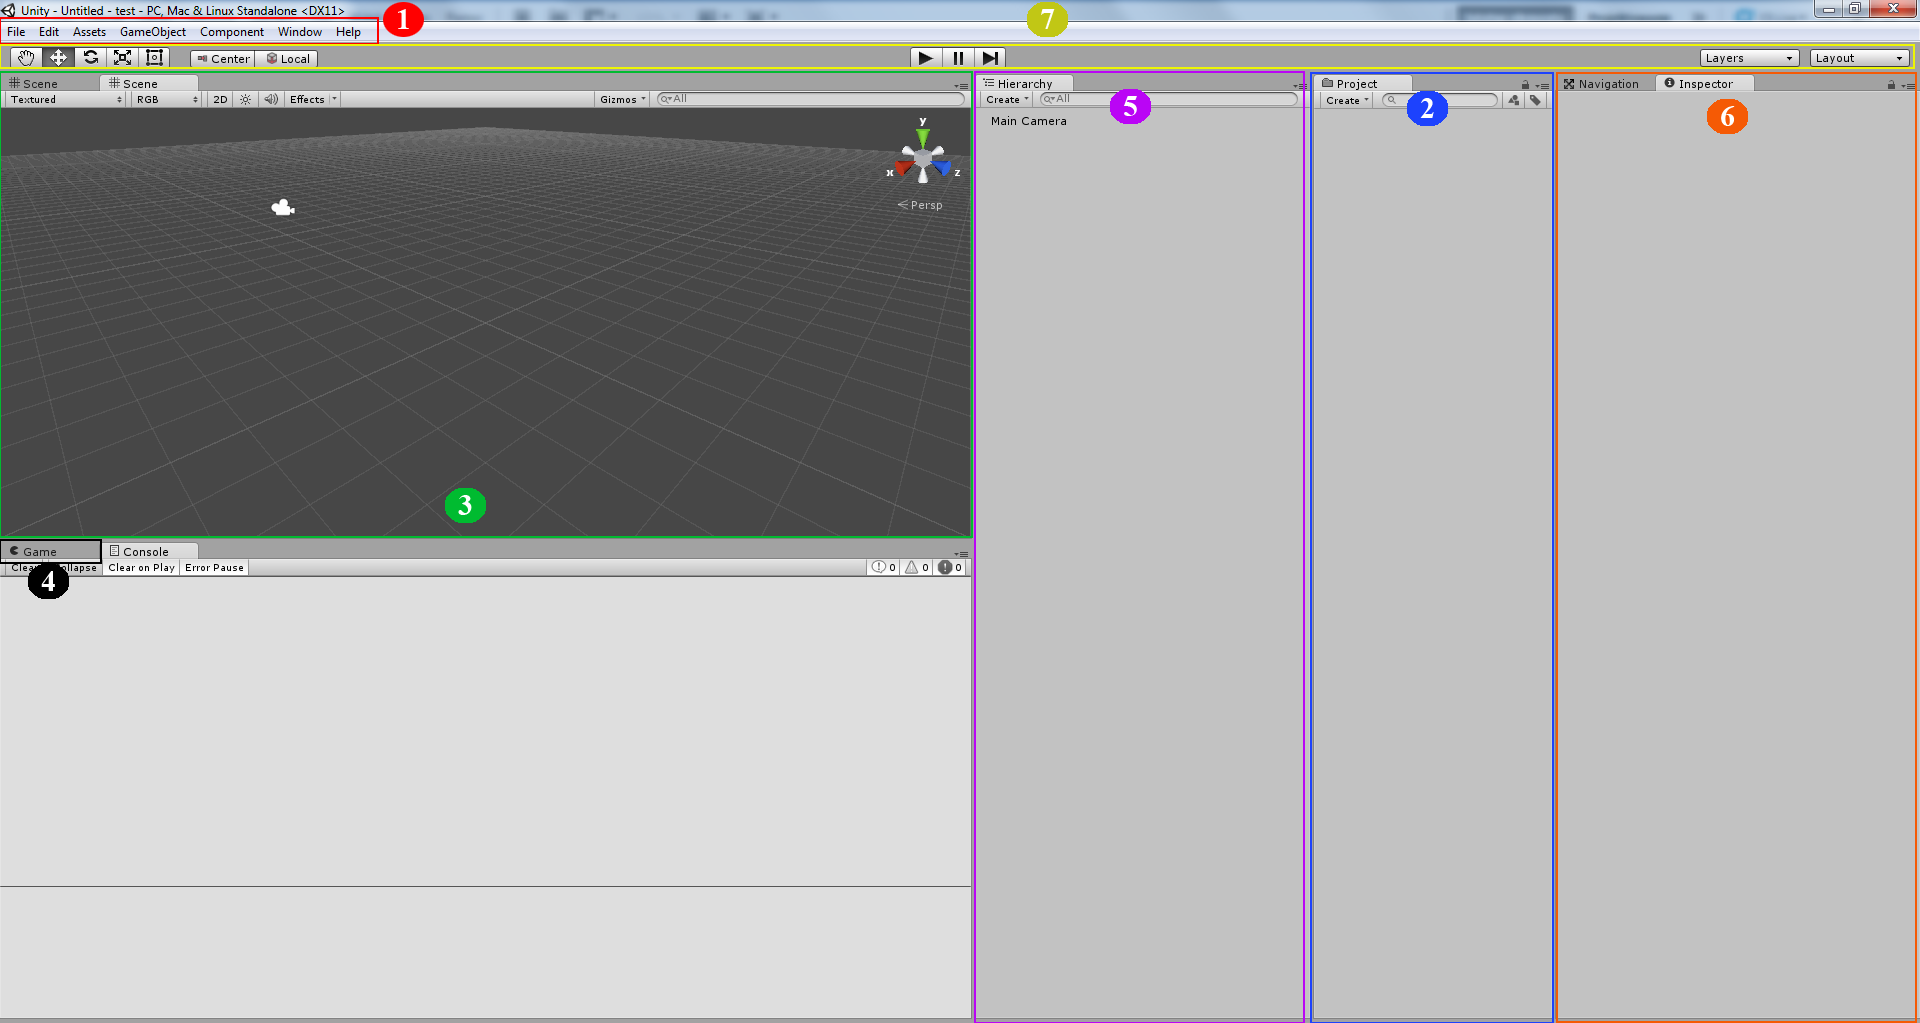
\includegraphics[scale=0.15]{Screeny/rodzial5screeny/ekran_glowny}
    \end{center}
    \caption{Podstawy - Unity - Ekran główny}
    Domyślny układ ekranu po stworzeniu nowego projektu, jeśli nie otwieraliśmy wcześniej na tym komputerze innego projekt Unity wraz z oznaczeniem poszczególnych okien.
    \source{Zrzut ekranu z Unity}
\end{figure}

Cyfry na zdjęciu oznaczają poszczególne okna:

\begin{enumerate}
  \item Pasek Menu – daje dostęp do bardziej zaawansowanych opcji, m.in. pozwala na dodawanie nowych okien, komponentów czy konfgurowanie całej aplikacji.
  \item  Project – tu umieszczone są wszystkie pliki jakie znajdują się w grze. Pliki możemy dodawać do projektu, przenosząc je bezpośrednio do tego okna, lub dodając je do folderu „Assets” w naszym projekcie.
  \item Scene – jest to przestrzeń 3D na której umieszczane są wszystkie obiekty znajdujące się w grze.
  \item Game – okno pozwalające na zobaczenie naszej gry w akcji po naciśnięciu przysiku „Play”. Domyślnie widać tylko niebieskie tło – jest to aktualny obraz z głównej kamery umieszczonej na scenie.
  \item Hierarchy – w tym oknie wypisana jest lista wszystkich obiektów znajdujących się na scenie. Pozwala nam na manipulowanie obiektem bez konieczności szukania go bezpośrednio na scenie.
  \item Inspector – wyświetla właściwości aktualnie zaznaczonego obiektu.
  \item  Pasek opcji – pozwala na zmianę opcji poruszania się po scenie, zmianę widoku przy zaznaczaniu obiektu, odpalenie naszej gry, zarządzanie warstwami i zmianę layoutu.
\end{enumerate}

 Ułożeniem poszczególnych okien można swobodnie manipulować poprzez przenoszenie zakładek lub zmianę layoutu z paska opcji. Możliwe jest też dodawanie nowych zakładek. Przy tworzeniu nowego projektu Unity wczyta ustawienia okien z poprzednio otwartego projektu, zaś przy otwieraniu innego projektu, okna ustawione będą tak jak ustawiła je osoba przy nim pracująca. Wszystkimi oknami można zarządzać klikając na nie, bądź korzystając z zakładki „Window” z paska menu (1).
\newpage
\section{Praca z obiektami i sceną}

Scena jest miejscem na którym umieszczać będziemy każdy element gry. Aby zapewnić sobie swobodną pracę, niezbędne jest opanowanie podstawowych zasad poruszania się po niej. Jak w każdej przestrzeni 3D, podstawowym sposobem przemiszczania się po scenie jest oddalanie/przybliżanie widoku oraz obracanie go w dowolnym kierunku. Po kliknięciu na scenę, aby przybliżyć bądź oddalić kamerę korzystamy z pomocy rolki myszki, lub wciskamy klawisz alt i przytrzymujemy prawy przycisk, poruszając jednocześnie myszką w tył lub przód. Aby rotować widok, przytrzymujemy alt i lewy przycisk poruszając myszką w dowolnym kierunku. Aby mieć na czym operować niezbędne jest stworzenie Game Objectu. Aby to zrobić klikamy lewym przyciskiem myszki w oknie Hierarchy (5), lub klikając Game Object z paska menu (1) i i wybieramy „Create empty”.

Stworzy nam to na scenie pusty obiekt, a w hierarchii pojawi się jego nazwa i możliwość zaznaczenia go. Po zaznaczeniu zobaczymy jego pozycję na scenie reprezentowaną przez mały sześcian i 3 strzałki różnego koloru. Kolory strzałek oznaczają różne osie - zielona oś Y, symbolizująca ruch góra/dół, czerwona oś X, symbolizująca ruch lewo/prawo, oraz niebieska oś Z symbolizująca głębię.

Jako, że obiekt posiada już domyślny komponent Transform, możliwe są operacje na jego prezentacji w przestrzeni. Na pasku opcji (7), poczynając od lewej znajduje się 5 przycisków do wykonywania tych operacji i odpowiedniego przełączania się między nimi. Wszystkie tryby można uruchamiać także  przy pomocy skrótów klawiszowych.

Pierwszy przycisk od lewej pozwala nam na poruszanie samym widokiem w przestrzeni przy pomocy myszki, nawet gdy obiekt jest zaznaczony.

\begin{figure}[!htb]
    \begin{center}
    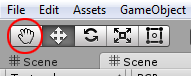
\includegraphics[scale=0.4]{Screeny/rodzial5screeny/drag_option}
    \end{center}
    \caption{Podstawy - Unity - Opcja poruszania kamery}
    \source{Zrzut ekranu z Unity}
\end{figure}

Drugi przycisk umożliwia nam na zmienianie pozycji obiektu w przestrzeni. Możemy swobodnie poruszać obiektem klikając na kwadrat, bądź jeśli chcemy poruszać obiekt po konkretnej osi – na odpowiednie strzałki. Można uruchomić ten tryb korzystając z przycisku „W” na klawiaturze.

\begin{figure}[!htb]
    \begin{center}
    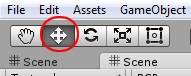
\includegraphics[scale=0.4]{Screeny/rodzial5screeny/move_option}
    \end{center}
    \caption{Podstawy - Unity - Opcja przemieszczania obiektu}
    \source{Zrzut ekranu z Unity}
\end{figure}

Trzeci przycisk służy to zmiany rotacji obiektu w przestrzeni. Po uruchomieniu tego trybu zobaczymy, że wygląd osi zmienił się na kształt sfery. Rotację wykonujemy tak samo jak zmianę pozycji poprzez klikanie na odpowiednie osie.

\begin{figure}[!htb]
    \begin{center}
    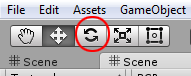
\includegraphics[scale=0.4]{Screeny/rodzial5screeny/rotate_option}
    \end{center}
    \caption{Podstawy - Unity - Opcja rotowania obiektu}
    \source{Zrzut ekranu z Unity}
\end{figure}

Czwarty przycisk służy do zmiany skali obiekty. Zmianę wykonujemy poprzez naciśnięcie na małe szcześciany widoczne na osiach.

\begin{figure}[!htb]
    \begin{center}
    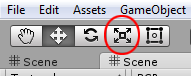
\includegraphics[scale=0.4]{Screeny/rodzial5screeny/scale_option}
    \end{center}
    \caption{Podstawy - Unity - Opcja skalowania obiektu}
    \source{Zrzut ekranu z Unity}
\end{figure}

Ostatni przycisk służy do obsługi tzw. Rect Transform i wychodzi poza zakres podstawowy i nie będzie omawiany w tym rozdziale.

\begin{figure}[!htb]
    \begin{center}
    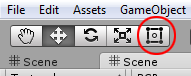
\includegraphics[scale=0.4]{Screeny/rodzial5screeny/recttrans_option}
    \end{center}
    \caption{Podstawy - Unity - Opcja Rect Transform }
    \source{Zrzut ekranu z Unity}
\end{figure}

Mimo, że puste obiekty same w sobie nic nie robią to są używane równie często, co obiekty z komponentami. Wynika to z faktu, że można je zagnieżdżać tak samo jak foldery – przenosząc jeden obiekt na drugi w oknie hierarchii. Ma to kilka zastosowań. Po pierwsze pozwala na zorganizowanie obiektów na scenie, która może składać się z tysięcy obiektów i nawigacja między nimi mogłaby być bardzo kłopotliwa. Przykładowo, posiadając obiekt „samochód”, obiekty takie jak „koło”, „karoseria”, „lampy” itd. powinny być umieszczone w tym obiekcie. Dzięki temu, poruszając „samochodem”, jednocześnie przemieścimy o tę samą wartość „koła”, „karoserię” i „lampy”. Te obiekty nazywane są obiektami potomnymi, ang. Child Objects. Samochód jest w tym momencie rodzicem, ang. Parent Object. Ma to szczególne znaczenie przy skomplikowanych obiektach, gdzie przemieszczanie każdego z nich oddzielnie byłoby bardzo niepraktyczne. Ta sama zasada dotyczy się rotacji i skali. Modyfikacja obiektu potomnego nie wpływa za to na jego rodzica. Drugim ważnym zastosowaniem obiektów potomnych jest możliwość odwoływania się do nich poprzez rodzica. Oznacza to, że skrypty umieszczone w obiekcie, posiadającym jedno lub wiele dzieci, mogą za jednym zamachem kontrolować wszystkie z nich.

\begin{figure}[!htb]
    \begin{center}
    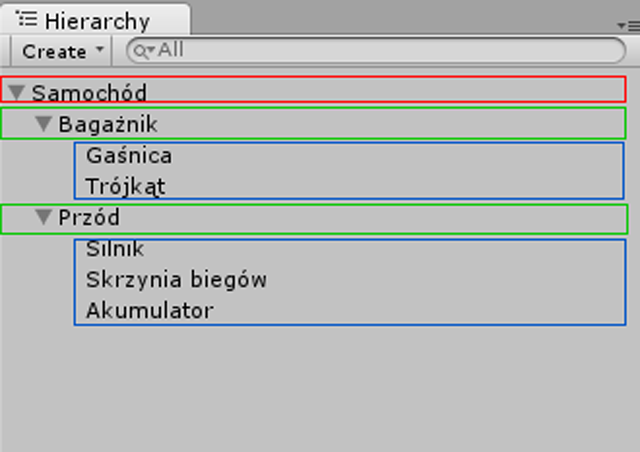
\includegraphics[scale=0.25]{Screeny/rodzial5screeny/przyklad_relacji_rodzic_dziecko}
    \end{center}
    \caption{Podstawy - Unity - Relacja Rodzic - Dziecko}
Kolorem czerwonym oznaczono obiekt gry, będący rodzicem znajdujących się w nim obiektów: bagażnik i przód, oznaczonych kolorem zielonym. Bagażnik i przód są jednocześnie dziećmi obiektu samochód jak i rodzicami obiektów: gaśnica, trójkąt, silnik, skrzynia biegów oraz akumulator oznaczonych kolorem niebieskim.
    \source{Zrzut ekranu z Unity}
\end{figure}

Każdy obiekt który umieszczamy na scenie automatycznie pojawia się w oknie hierarchii. Zaznaczenie obiektu w hierarchii zaznaczy nam obiekt na scenie i vice versa, a także wyświetli wszystkie komponenty podpięte do tego obiektu w oknie inspektora (4).

\section{Okno inspektora i komponenty}

Unity daje nam dostęp do kilku niepustych obiektów pozwalających na szybkie rozpoczęcie pracy. Aby stworzyć taki obiekt klikamy na zakładkę „GameObject” z paska menu (1). Do wyboru mamy kilka obiektów. Wybieramy 3D Object → Cube, co stworzy nam na scenie obiekt w kształcie szarego sześcianu i automatycznie go zaznaczy. W oknie inspektora (5) poza komponentem Transform dostrzeżemy też trzy inne. Mesh Filter pobiera informacje na temat siatki modelu i przekazuje je do ostatniego komponentu, Mesh Renderera, który tę siatkę renderuje. Box Collider tworzy kolider wokół siatki który pozwala na interakcje z innymi obiektami – zostanie on omówiony w dalszej części tego rozdziału. Większość komponentów zawiera w sobie dodatkowe opcje umożliwiające modyfikację ich działania. Przykładowo, zmiana wartości x, y  lub z w komponencie Box Collider zmieni jego rozmiary podobnie jak właściwość Scale w komponencie Transform. Komponenty można dodawać, usuwać, zmieniać ich kolejność oraz kopiować, klikając prawym przyciskiem na jego nazwie lub klikając przycisk Add component na dole inspektora. Przykładowo, usunięcie komponentu Mesh Renderer z naszego obiektu, sprawi, że jego ściany przestaną się wyświetlać jednak nadal będą możliwe kolizje z innymi obiektami.
Istnieje też możliwość wyłączenia danego komponentu (nie będzie on działał, ale nie będzie też usunięty) poprzez kliknięcie checkboxa  oraz ukrycie właściwości przy pomocy małej strzałeczki, oba usytuowane tuż obok jego nazwy.

Za każdym razem gdy zaznaczymy nowy obiekt, w inspektorze wyświetlą się jego komponenty. Klikając na małą ikonkę w górnym prawym rogu inspektora, możemy zablokować widok na komponentach aktualnie wybranego obiektu.

\section{Skrypty}

Unity umożliwia nam rozszerzanie swojej funkcjonalności oraz kontrolę zachowań poprzez skrypty. Do wyboru mamy trzy języki – C\#, Unity Script (zmodyfikowana wersja Java Script) oraz Boo, który jednak przestał być wspierany od wersji 5.0 . Zaleca się aby w ramach danego projektu używać tylko jednego języka aby uniknąć problemów z kompatybilnością.
Największą popularnością cieszy się C\#. Może też pochwalić się najlepszą dokumentacją, dlatego jest zalecany osobom zaczynającym pracę z Unity. Także wszystkie skrypty wykorzystane w tej pracy napisane zostały w tym języku.

Skrypty tworzymy klikając prawym przyciskiem myszy w oknie projektu i wybierając opcję  Create    → C\# Script z menu kontekstowego. Tak samo tworzymy foldery oraz wewnętrzne assety. Po wpisaniu nazwy (zaczynającej się dużą literą, gdyż mamy do czynienia z nazwą klasy) możemy kliknąć dwukrotnie lewym przyciskiem na skrypt, aby go otworzyć. Domyślnie uruchomi to środowisko programistyczne Mono Develop (możemy korzystać z dowolnego edytora, wymaga to jednak wcześniejszej konfiguracji, lub bezpośredniego otwierania pliku z folderu projektu). Każdy nowy skrypt posiada taki szablon (można go zmienić w pliku ScriptTemplates w folderze Unity):

\newpage
\begin{lstlisting}
using UnityEngine;
using System.Collection;

public class NazwaSkryptu: MonoBehaviour {

	//use this for initialization
	void Start () {

	}

	//Update is called once per frame
	void Update() {

	}
}
\end{lstlisting}

Każdy skrypt domyślnie dziedziczy po klasie MonoBehaviour, która  udostępnia wszystkie funkcje jakie oferuje nam Unity. Ta klasa jest niezbędna aby móc dodawać skrypty do Game Objectów.

Funkcja Start() wywołuje się zawsze, jednorazowo przy załadowywaniu nowej sceny. Jest wykorzystywana do inicjalizacji wszelkich ustawień i zachowań na początku gry. Jeśli na scenie znajduje się wiele obiektów z podpiętymi różnymi skryptami posiadającymi tę funkcję, dla każdego  z nich ta funkcja wykona się raz, jednak kolejność ich wykonywania zależna będzie od rodzaju i specyfikacji urządzenia. Jeśli w jednym Starcie użyty będzie kod, który wymaga wpierw inizjalizacji Startu z innego skryptu może wystąpić tzw. efekt wyścigów. Może to spowodować wyświetlanie błędów, lub prowadzić do niechcianych i trudnych do przewidzenia zachowań.

Aby pomóc w uniknięciu tego typu problemów Unity udostępnia, trzy dodatkowe funkcje tego typu, które różnią się przede wszystkim kolejnością ich wykonywania dla wszystkich skryptów:

Awake() - wykonuje się jako pierwsze

OnEnable – wykonuje się gdy obiekt staje się aktywny, jeśli jest on aktywny od samego początku, to wykonuje się on tuż po Awake()

OnLevelWasLoaded() - wykonuje się tuż przed Startem, jednak nie bezpośrednio po starcie gry, a dopiero po zmianie sceny

Start() - wykonuje się jako ostatnia, tuż przed startem pierwszej klatki funkcji Update() jeśli obiekt jest aktywny

Istnieje specjalna funkcja DontDestroyOnLoad(), która powoduje, że obiekt nie jest niszczony pomiędzy scenami, oznacza to, że niektóre z powyższych funkcji nie wykonają się po zmianie sceny.

Funkcja Update() jest wywoływana co klatkę dla każdego obiektu z podpiętym skryptem. Wszystkie akcje w grze wymagające ciągłego wykonywania tego samego kawałka kodu, pisane są wewnątrz tej funkcji. Podobnie jak Start(), Update() posiada dwie funkcje tego samego typu:

FixedUpdate() - wykonuje się jako pierwsze. Wszystkie akcje związane z fizyką powinny być pisane wewnątrz tej funkcji. Jest to powodowane tym, że częstotliwość odświeżania klatek może się różnić w zależności od sprzętu i faktu, że w niektórych miejscach nasza gra może bardziej obciążać zasoby sprzętowe, a w innych mniej. W tej funkcji czas pomiędzy poszczególnymi klatkami jest zawsze taki sam, a obliczenia fizyczne opierają się na stałych wartościach. Losowy czas pomiędzy klatkami może powodować dziwne zachowania wynikające z problemów w obliczeniach.

Update() - wykonuje się drugie w kolejności. Wszystkie pozostałe akcje niezwiązane z fizyką powinny być pisane w tej funkcji.

LateUpdate() - jw. z tym, że wykonuje się dopiero gdy dana klatka została wykonana wcześniej we wszystkich Updateach

Powyższe funkcje są jednymi z najbardziej podstawowych i najczęściej wykorzystywanych funkcji w Unity, dlatego ich znajomość jest taka ważna.
\\
\\
Wszystkie komponenty są tak naprawdę skryptami. Oznacza to, że nie tylko możemy odwoływać się w napisanym przez nas skrypcie do dowolnego komponentu, ale możemy podpiąć dowolny skrypt do każdego obiektu w grze. Operując modyfikatorami dostępu możemy decydować do której właściwości możemy uzyskać dostęp i umożliwić jej zmianę z poziomu inspektora. Przeanalizujmy poniższy kod:

\newpage
\begin{lstlisting}

using UnityEngine;
using System.Collections;

public class Move : MonoBehaviour {

	int speedX = 3;
	public int speedY = 3;
	[SerializeField]
	int randomNumber = 8;
	void Update () {
		gameObject.transform.Translate (
			Time.deltaTime * speedX, 
			Time.deltaTime * speedY,
			0
		);
	}
}
\end{lstlisting}

Na początku zdefiniowaliśmy trzy zmienne. Pierwsza zmienna jest prywatna (jeśli nie zadeklarowaliśmy jawnego modyfikatora, to domyślnie zmienna jest prywatna). Prywatne zmienne nie są widziane przez inne skrypty. Nie są także widoczne z poziomu inspektora. Druga zmienna jest zmienna publiczną i można się do niej odwołać z poziomu innych skryptów. Dodatkowo będzie ona widoczna w inspektorze, i możliwa będzie jej modyfikacja bez konieczności jej zmiany w skrypcie. Raz tak zmieniona wartość jest na stałe zapamiętywana, do momentu jej ponownej zmiany w inspektorze lub modyfikacji kodu. Jeśli ta wartość zmienia się podczas samej gry, to ta zmiana zapamiętywana jest tylko do momentu zmiany sceny, bądź wyłączenia gry.

Mimo, że ostatnia zmienna także jest zmienną prywatną, to pole [SerializeField] sprawia, że będzie ona widoczna w inspektorze. Dalej jednak możliwość jej edycji będzie niedostępna.

Aby zapamiętać wartość zmiennej pomiędzy scenami należy użyć modyfikatora static, bądź skorzystać ze specjalnej klasy PlayerPrefs.

W funkcji Update(), która jak wiemy jest wykonywana co klatkę dodaliśmy możliwość poruszania się dla obiektu. Oto jak działa ta linia kodu: gameObject wkazuje na obiekt do którego aktualnie jest podpięty nasz skrypt, a transform odwołuje nas do komponentu Transform tego obiektu. Translate() jest nazwą funkcji w klasie Translate z której korzystamy. Translate przyjmuje parametr typu Vector3 (wkazuje on na punkt o danych x,y,z w przestrzeni trójwymiarowej). W tym wypadku podaliśmy wartości naszych zmiennych pomnożone przez wartość Time.deltaTime. Zrobiliśmy to, ponieważ bez tego nasz obiekt zmieniałby pozycję o 3 punkty w górę i 3 punkty w prawo co wyświetlaną klatkę. Ilość klatek w jednej sekundzie może sięgać nawet kilkuset, dlatego nasz obiekt poruszałby się z tak dużą prędkością, że byłoby to niewidoczne dla oka. Time.deltaTime dzieli naszą wartość odpowiednio do ilości wyświetlanych  klatek, dzięki czemu nasza pozycja będzie zmieniać się co sekundę zamiast co klatkę.

Skrypt podpinamy zaznaczając nasz obiekt (np. cube), i przenosząc skrypt z okna Projects do inspektora, lub klikając Add component i wyszukując nasz skrypt. Aby zobaczyć efekt działania skryptu nasz obiekt musimy znaleźć się w polu widzenia kamery. Domyślnie jeśli pozycja kamery nie była zmieniana, to umieszczenie obiektu w pozycji x=0, y=0,z=0 ustawi go na środku pola widzenia. Po naciśnięciu przycisku Play ujrzymy efekt działania naszego skryptu.

\begin{figure}[!htb]
    \begin{center}
    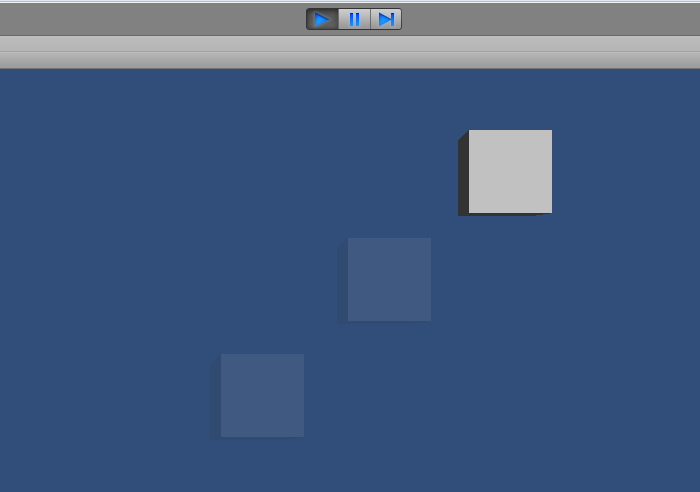
\includegraphics[scale=0.25]{Screeny/rodzial5screeny/moving_cube}
    \end{center}
    \caption{Podstawy - Unity - Przesuwanie sześcianu}
Jeśli poprzednie kroki zostały wykonane pomyślnie, po przycisku play powinniśmy ujrzeć tak wyglądający obiekt Cube, poruszjący się ze średnią prędkością w kierunku północno – wschodnim.
    \source{Zrzut ekranu z Unity}
\end{figure}


\newpage
\section{Kamera, światło i collidery}

Nawet bezpośrednio po stworzeniu nowego projektu nasza scena nie jest całkowicie pusta. W oknie hierarchii znajdziemy dwa obiekty: Main Camera oraz Directional Light. Pierwsze służy do przechwytywania i wyświetlania elementów sceny które ma widzieć gracz. Tak naprawdę poruszając się po scenie również korzystamy z kamery aby widzieć jej określoną część. Ilość kamer na scenie jest nieograniczona. Przy pomocy skryptów możemy przemieszczać kamery i dodawać do nich różne efekty. Odpowiednie ustawienie widoków pozwala nam na podgląd kilku, nawet zupełnie oddalonych od siebie fragmentów sceny na jednym ekranie. Dobrym przykładem wykorzystania dodatkowej kamery jest minimapa, używana często w strategiach czasu rzeczywistego lub w grach fabularnych.  Main Camera jak sama nazwa sugeruje pełni główną rolę w wyświetlaniu akcji gry i tylko ona wykorzystywana była w tej pracy.

Directional light służy do generowania odpowiedniego oświetlenia na scenie. Istnieje kilka rodzajów świateł i ich odpowiednie ustawienie jest kluczowe przy budowaniu świata gry. Directional Light cechuje się głównie tym, że jego położenie na scenie nie ma najmniejszego znaczenia, cała scena oświetlana jest równomiernie,za to rotacja ma wpływ na to z której strony to światło pada. Ten rodzaj światła praktycznie zawsze reprezentuje światło słoneczne na otwartych przestrzeniach. W zależności od pory dnia można modyfikować jego intensywność oraz inne parametry. Wbrew pozorom usunięcie światła ze sceny nie spowoduje, że obiekty będą kompletnie niewidoczne, a powiązane jest to z tzw. Ambient Light, opis którego nie wchodzi w zakres tego rozdziału.

Collider jest to komponent, który definiuje fizyczny kształt danego obiektu, niezbędny do wykrywania kolizji z innymi obiektami. Często przybiera on kształt siatki modelu który został podpięty do danego obiektu. Ze względu na fakt, że skomplikowane kolidery są bardzo procesożerne, bardzo często korzysta się z tzw. prymitywnych koliderów – w kształcie sfer, sześcianów i kul. Obiekt może posiadać dowolną ich liczbę, dlatego skomplikowane modele z reguły składają się z wielu prymitywnych koliderów. Efekt tego bardzo często widać w grach, gdy część postaci przenika przez ścianę, lub jesteśmy blokowani przez przeszkodę nie dotykając jej. Odpowiednie ustawienie koliderów ma więc kluczowe znaczenie i pozwala uniknąć tzw. Glitchy, gdy w pewnych miejscach obiekty przechodzą przez siebie mimo że nie powinny. Collidery opierają się mocno na fizyce, co także bywa przyczyną błędów, np. gdy obiekty zderzają się ze sobą przy zbyt dużej prędkości. Bardziej zaawansowane kolidery takie jak Mesh Collider, zapewniają lepszą dokładność niż kolidery prymitywne, jest to jednak okupione większym zużyciem zasobów sprzętowych.

Collidery dzielą się jeszcze na dwa  oddzielne typy niezależnie od ich kształtu. Są to tzw. Trigger Collidery i Collision Collidery. Pomiędzy tymi dwoma typami możemy przełączać się przy pomocy checkboxa „isTrigger” we właściwościach komponentu. Różnica między nimi polega na tym, że w przypadku tego pierwszego, gdy dwa obiekty zetkną się to zostanie to odnotowane i przy pomocy odpowiedniej funkcji OnTriggerEnter() będziemy mogli je obsłużyć, lecz obiekty przenikną się i nie będą miały wpływu na swoją pozycję w przestrzeni. W wypadku gdy opcja „isTrigger” jest odznaczona, oba obiekty zderzą się i w zależności od ich parametrów fizycznych nastąpi odpowiednia reakcja. Ten typ zderzenia obsługujemy funkcją OnCollissionEnter().

Jako, że Collidery opierają się na fizyce, obiekty z nich korzystające muszą posiadać odpowiednie cechy fizyczne. Aby nadać te cechy obiektowi musimy dodać do niego komponent Rigidbody. Pozwala on m.in. na ustalenie masy obiektu i czy działa na niego grawitacja.

Co ciekawe Unity korzysta aż z dwóch systemów do obsługi fizyki, jeden dla obiektów 2D i drugi dla obiektów 3D. Każdy komponent korzystający z fizyki 3D ma swój odpowiednik 2D. Aby uzyskać do niego dostęp przy nazwie komponentu/funkcji dopisujemy na końcu 2D, np. Rigidbody2D lub OnCollisionEnter2D. Obiekty 2D nie mogą kolidować z obiektami 3D, a korzystanie z funkcji dedykowanej 2D, przy trójwymiarowym modelu korzystającym z kolidera 3D zwróci błąd.

Korzystając z koliderów trzeba bardzo uważać by nie zagnieżdżać wielu koliderów w jednym miejscu i unikać ich nadużywania, gdyż może to prowadzić do poważnych problem wydajnościowych.

Poniższy screen przedstawia przykładowy model korzystający z kilku podstawowych koliderów:

\begin{figure}[!htb]
    \begin{center}
    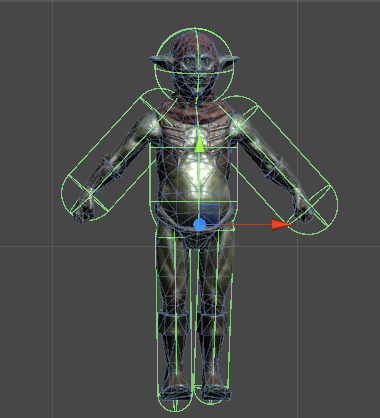
\includegraphics[scale=0.25]{Screeny/rodzial5screeny/model_prymitywne_kolidery}
    \end{center}
    \caption{Podstawy - Unity - Prymitywne kolidery}
Model składa się z koliderów cylindrycznych oraz kołowych. Kolidery prymitywne zapewniają zadowolającą dokładność przy wykrywaniu kolizji, nie obciążając przy tym zbytnio zasobów sprzętowych.
    \source{Zrzut ekranu z Unity}
\end{figure}

Temat Colliderów zamyka podstawowe zagadnienia związane z Unity.

\chapter{Podstawy tworzenia gier w Unreal Engine}

Ten rozdział poświęcony jest podstawowym elementom Unreal Engine. Nie jest to lista pełna, opisuje jedynie najważniejsze elementy potrzebne do tworzenia gier.

\section{Rozpoczęcie projektu}

Rozpoczęcie tworzenia nowej gry w Unreal Engine jest bardzo proste. Po uruchomieniu silnika, wystarczy kliknąć w zakładkę „New Project”.

\begin{figure}[!htb]
    \begin{center}
    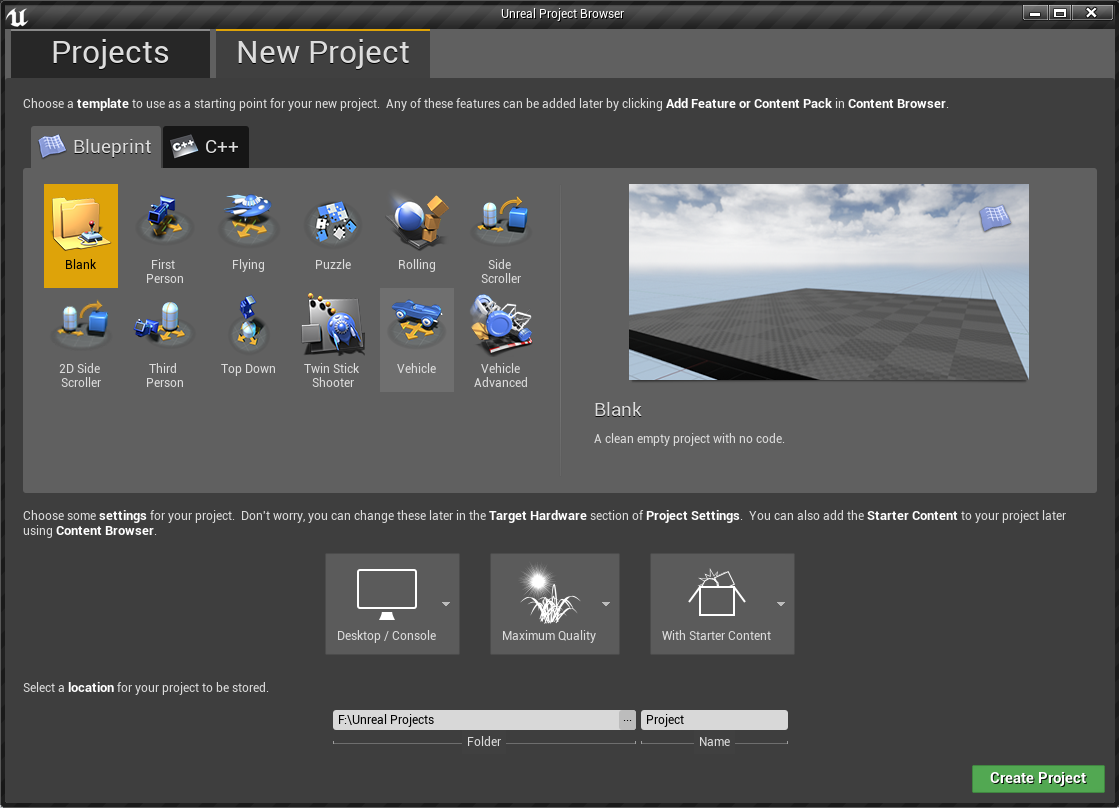
\includegraphics[scale=0.35]{Screeny/New_project}
    \end{center}
    \caption{Podstawy - UE - Nowy Projekt}
    \source{Zrzut ekranu z UnrealEngine}
\end{figure}

Przeniesie nas to na ekran, na którym wybieramy wstępne ustawienia naszego projektu. Pierwszą decyzją jaką musimy podjąć, to w jaki sposób będziemy radzić sobie z logiką- poprzez pisanie kodu w C++, czy ustawianie bloków logicznych w tzw. Blueprint’ach.

Blueprint to system oparty na wizualnym przesuwaniu bloków logicznych, zamiast ręcznego pisania kodu. System ten jest bardzo prostu w obsłudze. Każdy obiekt wymagający logiki może posiadac odpowiadający mu Blueprint. Pozwala to tworzenie skomplikowanej logiki bez konieczności pisania ogromnej ilości kodu. Blueprint, podobnie jak klasa w obiektowych językach programowania, może zostać użyty wielokrotnie. Na przykład stworzenie Blueprintu lampy, pozwoli ustawić ją w wielu miejscach w grze. Każda będzie działała tak samo.

Należy zaznaczyć, że wybór jednego sposobu, nie wyklucza nas całkowicie z korzystania z drugiej opcji. Jest to po prostu wskazanie, że preferujemy radzić sobie z logiką w taki, a nie inny sposób.
Warto również pamiętać, że Unreal Engine nie posiada dedykowanego edytora kodu C++. Jeśli chcemy programować w tym języku potrzebujemy zewnętrznego edytora, np. Visual Studio.

Kolejnym krokiem jest wybór schematu, jakim będziemy się posługiwać. W zależności od tego jaką grę tworzymy, scemat może zdecydowanie uprościć pierwsze kroki w edytorze gry (np. Schemat „2D Side Scroller”, stworzony z myślą o grach dwuwymiarowych, od razu będzie miał odpowiednio ustawioną kamerę). Istnieje również możliwość stworzenia pustego projektu, poprzez wybór opcji „Blank”.

Ostatnim krokiem jest wybór platformy na jaką chcemy tworzyć grę, jakość grafiki (istotna w przypadku słabszych sprzętów), oraz czy chcemy, by projekt zaimportował wstępne zasoby przygotowane dla nas przez Epic Games. Zasoby te składają sie między innymi z podstawowych animacji, tekstur i odgłosów.
Po dokonaniu wyboru pozostaje już tylko nazwać projekt i wcisnąć „Create Project”.

\newpage
\section{Ekran główny}

\begin{figure}[!htb]
    \begin{center}
    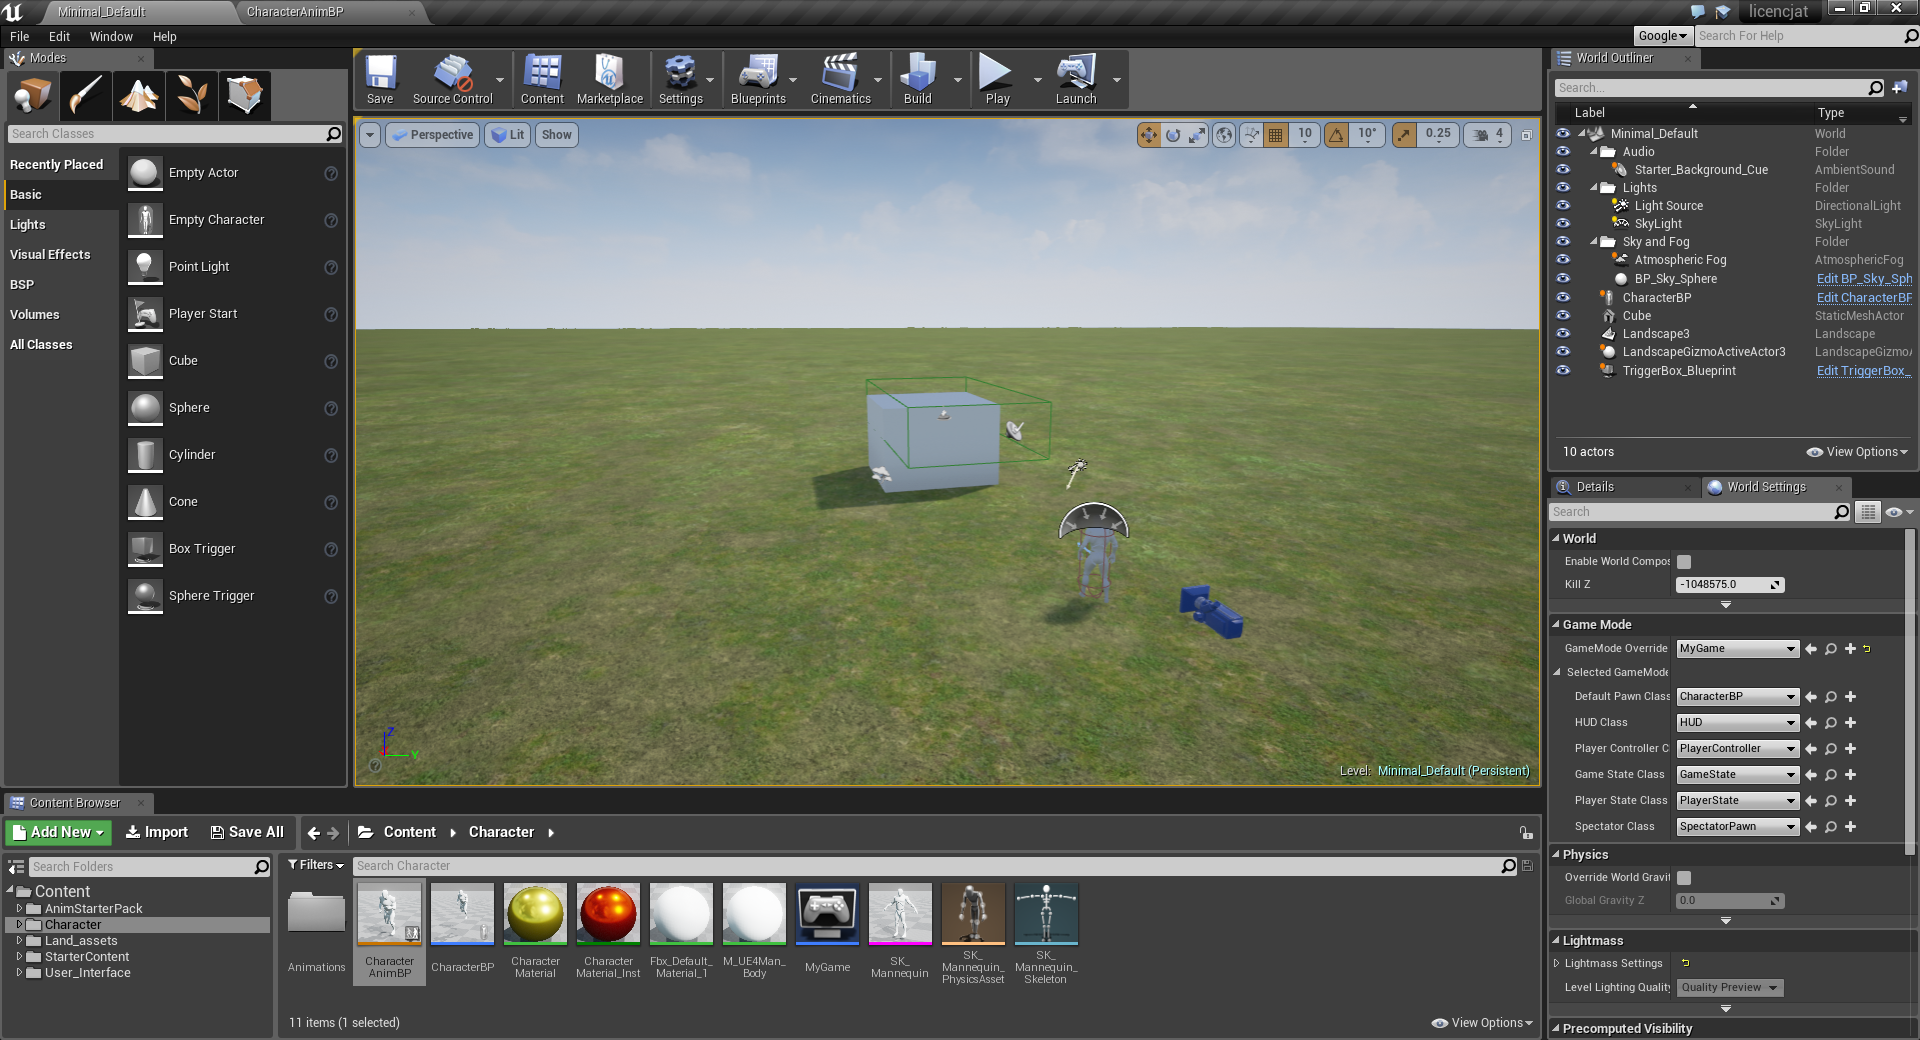
\includegraphics[scale=0.25]{Screeny/Main}
    \end{center}
    \caption{Podstawy - UE - Ekran Główny}
    \source{Zrzut ekranu z UnrealEngine}
\end{figure}

Po stworzeniu projektu, załaduje nam się ekran główny Unreal Engine. Na jego środku widzimy podgląd sceny nad którą obecnie pracujemy. Scena jest po prostu jednym z pozomów naszej gry.
Pod ekranem podglądu mamy przeglądarkę plików znajdujących się w projekcie.

Po prawej stronie znajduje się lista obiektów, znajdujących się w obecnej scenie. Jako obiekt traktowane jest wszystko, od podłoża, przez postacie, aż po źródło światła, czy sam dźwięk.
Pod listą obiektów znajdują się szczegóły obecnie wybranego obiektu.

Po lewej stronie znajdują się narzędzia do tworzenia obiektów. Jest to pięć zakładek zawierających w sobie wszystkie potrzebne opcje do tworzenia świata gry. Od tworzenia oświetlenia i prostych kształtów po nakładanie tekstur i modyfikowanie terenu.

\section{System Persona i Animacje}
Persona jest bardzo rozbudowanym narzędziem do edycji animacji. To jeden z najważniejszych systemów silnika. To dzięki niemu możemy określić gdzie, kiedy i w jakich warunkach  rozpoczyna się i kończy każda animacja w grze, od postaci, aż po spadające liście.

Trzeba pamiętać, że Unreal Engine nie posiada w sobie narzędzi do tworzenia animacji. Potrafi je tylko w pewnym stopniu modyfikować. Animacje należy importować z zewnętrznych programów do tworzenia animacji, takich jak Maya, lub Blender. Wystarczy przeciągnąć animację do przeglądarki plików.

Aby uruchomić Personę, wystarczy dwa razy kliknąć w edytorze na dowolny obiekt związany z animacją (np. sama animacja, lub Blueprint animacji).

Sam system składa się z czterech głównych trybów, ukazanych w prawym górnym rogu okienka.

\begin{figure}[!htb]
    \begin{center}
    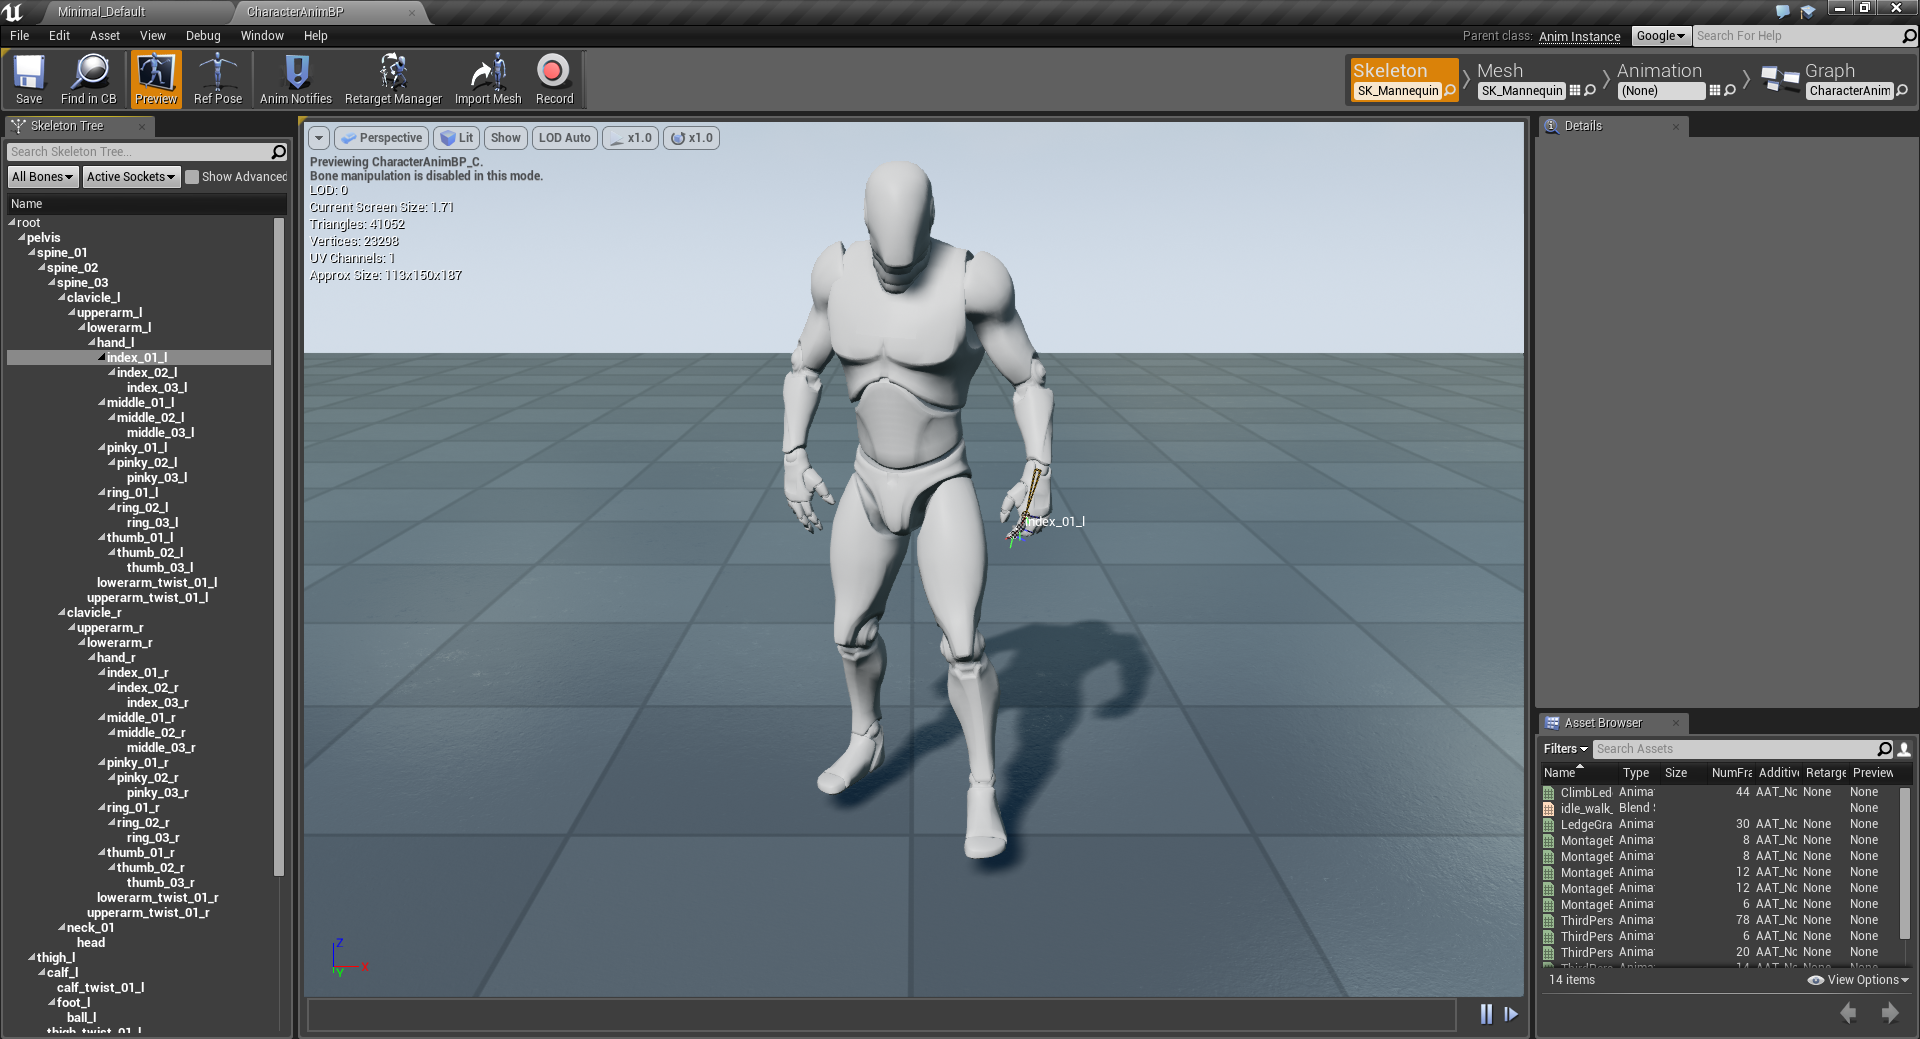
\includegraphics[scale=0.25]{Screeny/Skeleton}
    \end{center}
    \caption{Podstawy - UE - Szkielet}
    \source{Zrzut ekranu z UnrealEngine}
\end{figure}

Pierwszy tryb odpowiada za edycję szkieletu animacji. Po uruchomieniu od razu rzuca się w oczy podgląd animacji na środku okna. Rejestruje on jej obecny stan. Podgląd ten jest częścią wspólną wszystkich trybów pracy w Personie. Po lewej stronie wyświetlone są wszystkie wnęki i połączone z nimi kości obecnego modelu. Można dowolnie dodawać je i usuwać ze szkieletu postaci. Jest to szczególnie przydatne, gdy chcemy aby nasza postać np. chwytała broń. Wystarczy, że dodamy wnękę do ręki szkieletu, a nasza postać będzie już w stanie wykonać tę czynność.

\begin{figure}[!htb]
    \begin{center}
    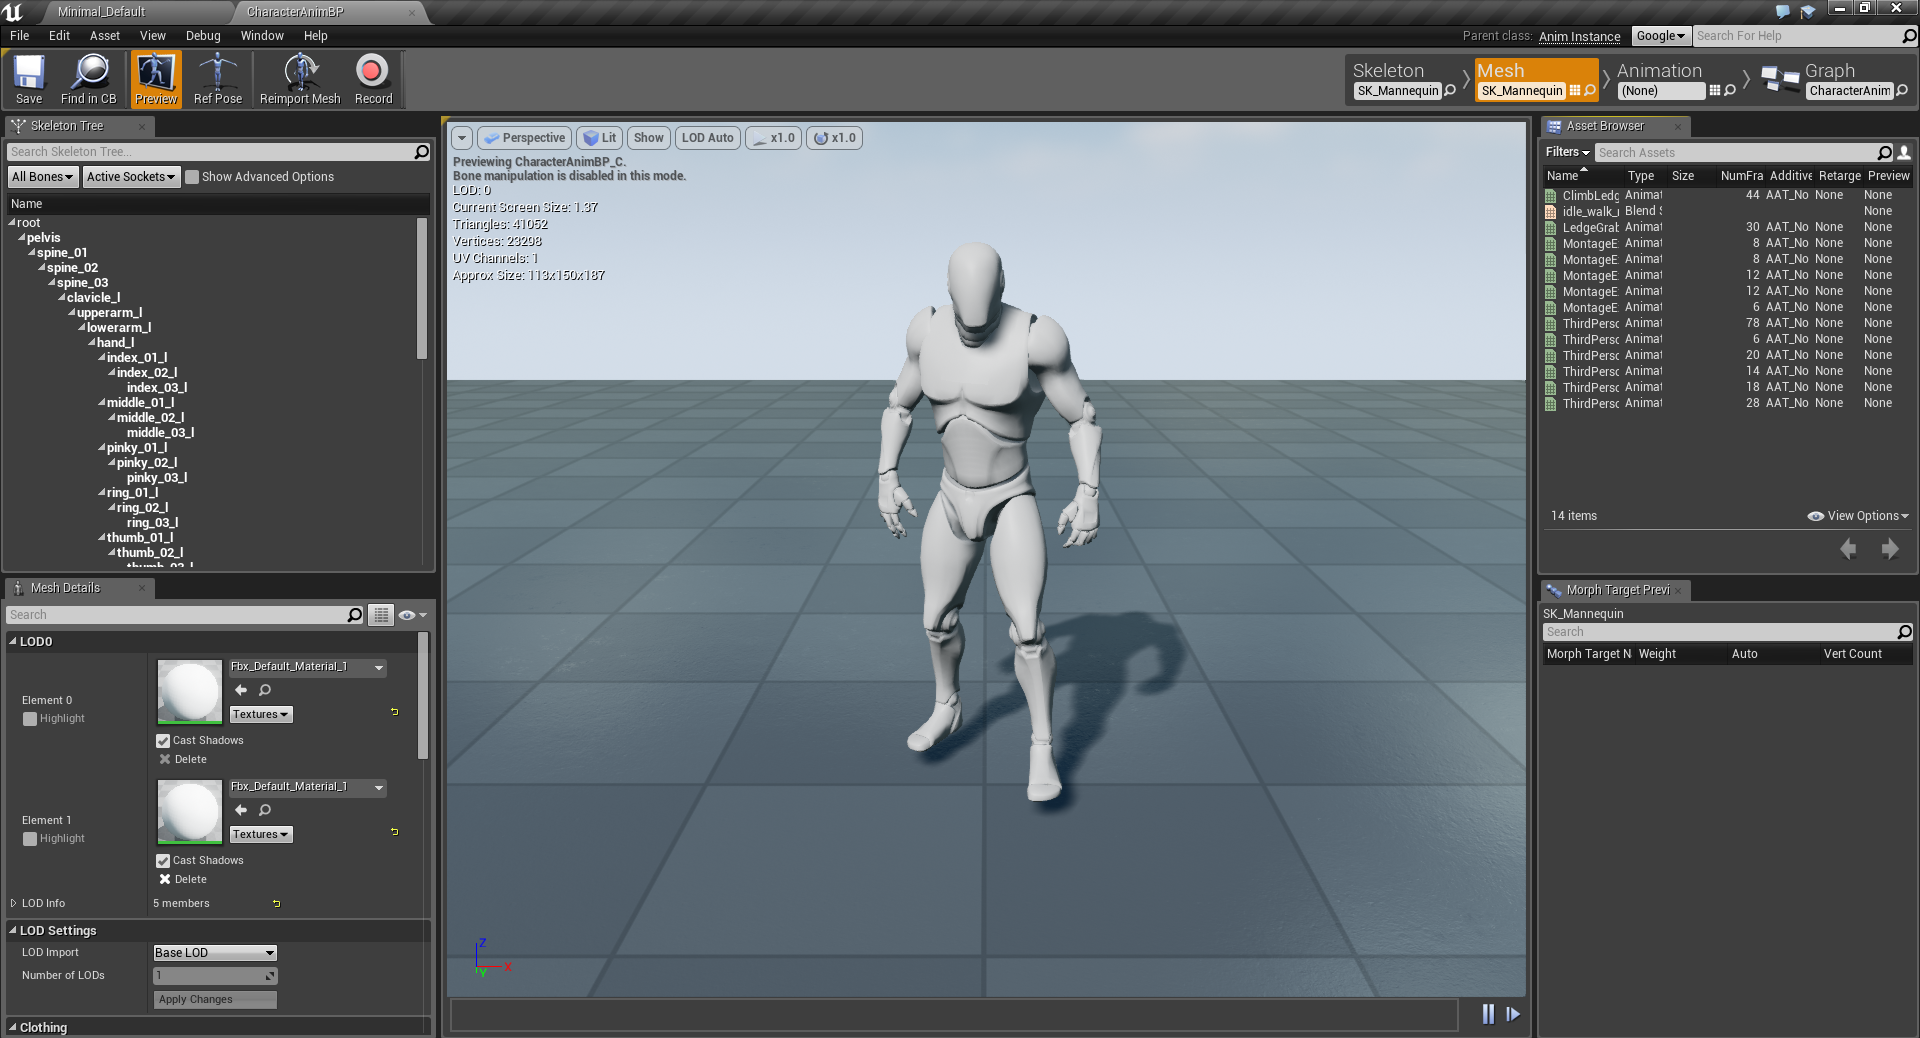
\includegraphics[scale=0.25]{Screeny/Mesh}
    \end{center}
    \caption{Podstawy - UE - Mesh}
    \source{Zrzut ekranu z UnrealEngine}
\end{figure}

Kolejny ekran jest odpowiedzialny za edycję meshy. Mesh to nic innego ja zbiór punktów, linii i wieloboków, które składają się na ostateczny kształt obiektu.
Ten tryb ma wiele wspólnego z poprzednim. Ma jednak dwa ważne menu, niedostępne w innych podsystemach Persony – „Mesh Details” i „Morph Target Preview”.
Mesh Details odpowiada głównie za edycję mesh’u nad którym obecnie pracujemy. Możemy dodać do niego nowe tekstury, kontrolować właściwości fizyczne (np. Płaszcz łopoczący na wietrze), lub umożliwić kolizję z innymi obiektami w grze.
Morph Target Preview pozwala na podgląd wszystkich modyfikacji mesha. Możemy na przykład zmienić wyraz twarzy postaci, zapisać go i użyć w odpowiedniej sytuacji, a potem obejrzeć go bez konieczności trwałej zmiany samego mesha.

\newpage
\begin{figure}[!htb]
    \begin{center}
    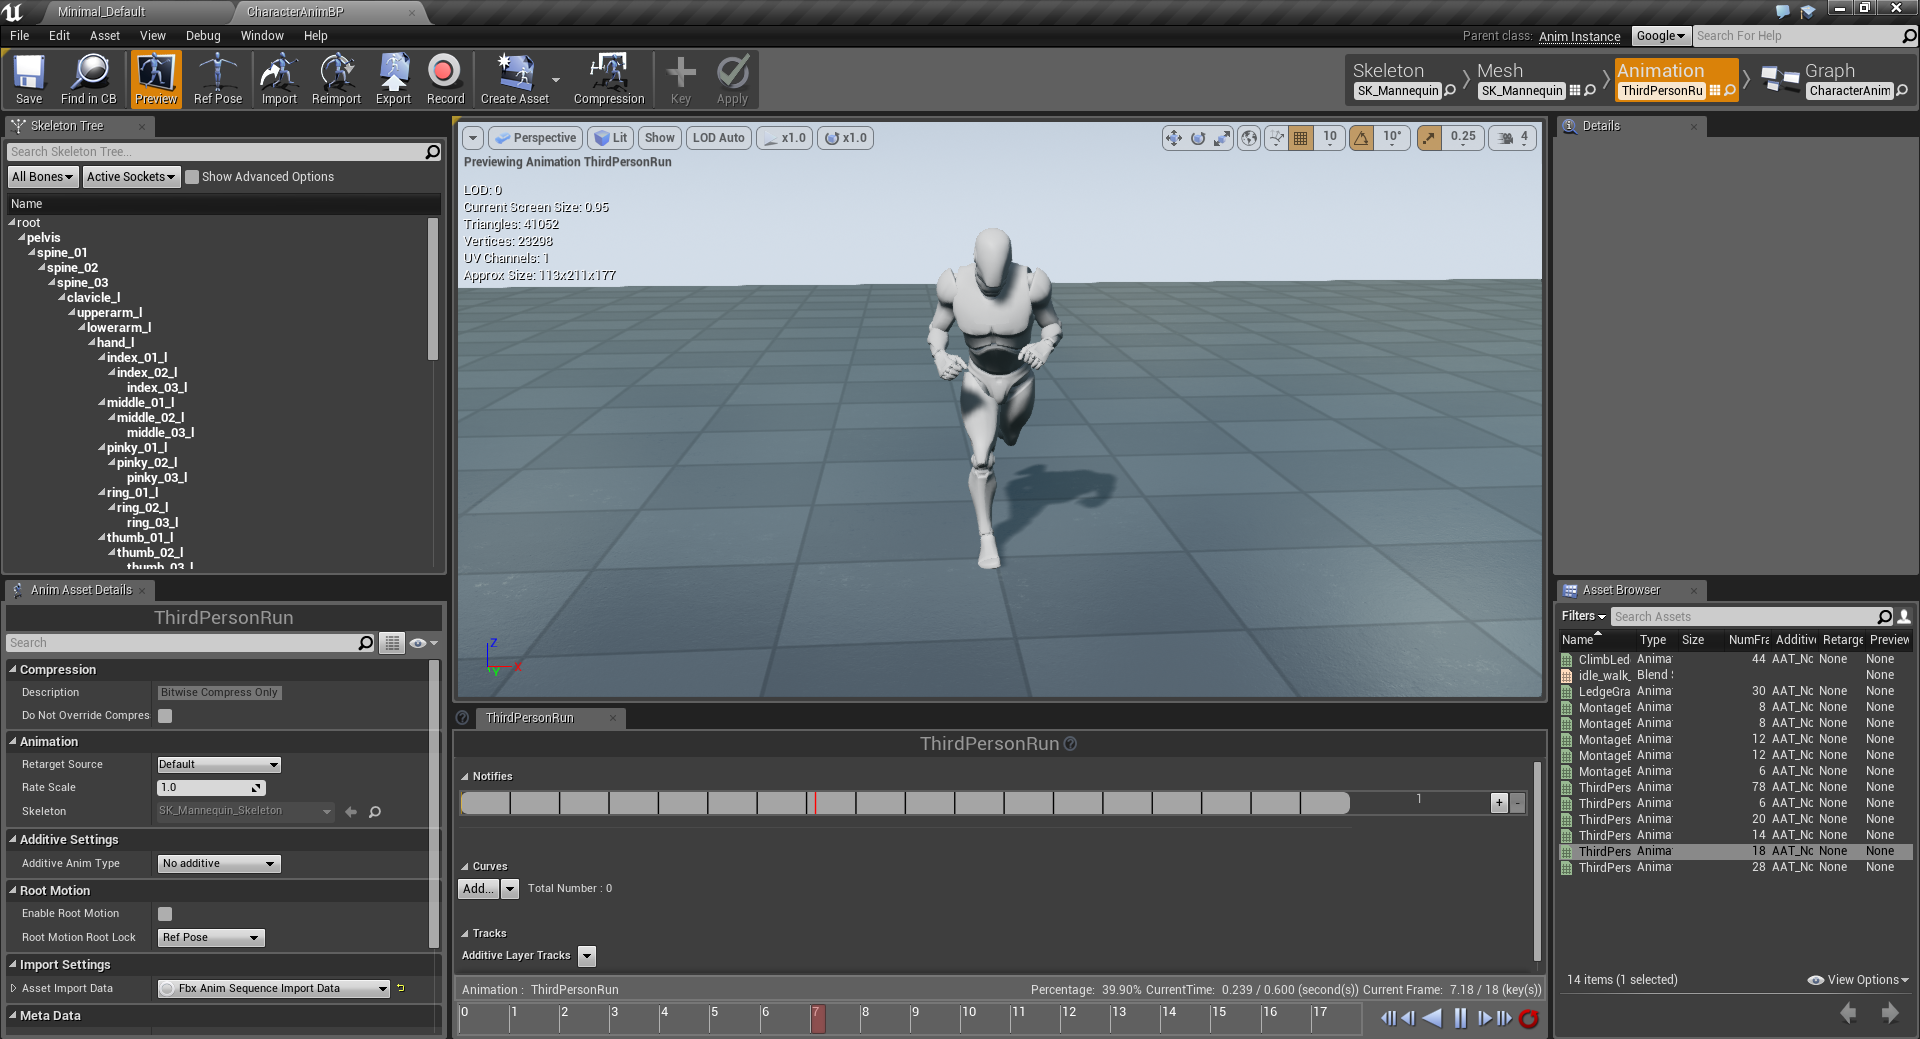
\includegraphics[scale=0.25]{Screeny/Animation}
    \end{center}
    \caption{Podstawy - UE - Animacja}
    \source{Zrzut ekranu z UnrealEngine}
\end{figure}

Następny tryb daje nam kontrolę nad animacjami. W lewym dolnym rogu widzimy szczegółowe ustawienia wybranej w tym momencie animacji.
Pod oknem podglądu animacji widzimy narzędzie dzięki któremu możemy przewijać wybraną animację klatka po klatce. Po wybraniu interesującego nas momentu animacji, możemy dodać różnego rodzaju efekty np. w momencie, gdy model w animacji biegu dotyka ziemi, możemy dodać odgłos kroku, albo efekt, który wznieci tuman kurzu pod stopą modelu.

\newpage
\begin{figure}[!htb]
    \begin{center}
    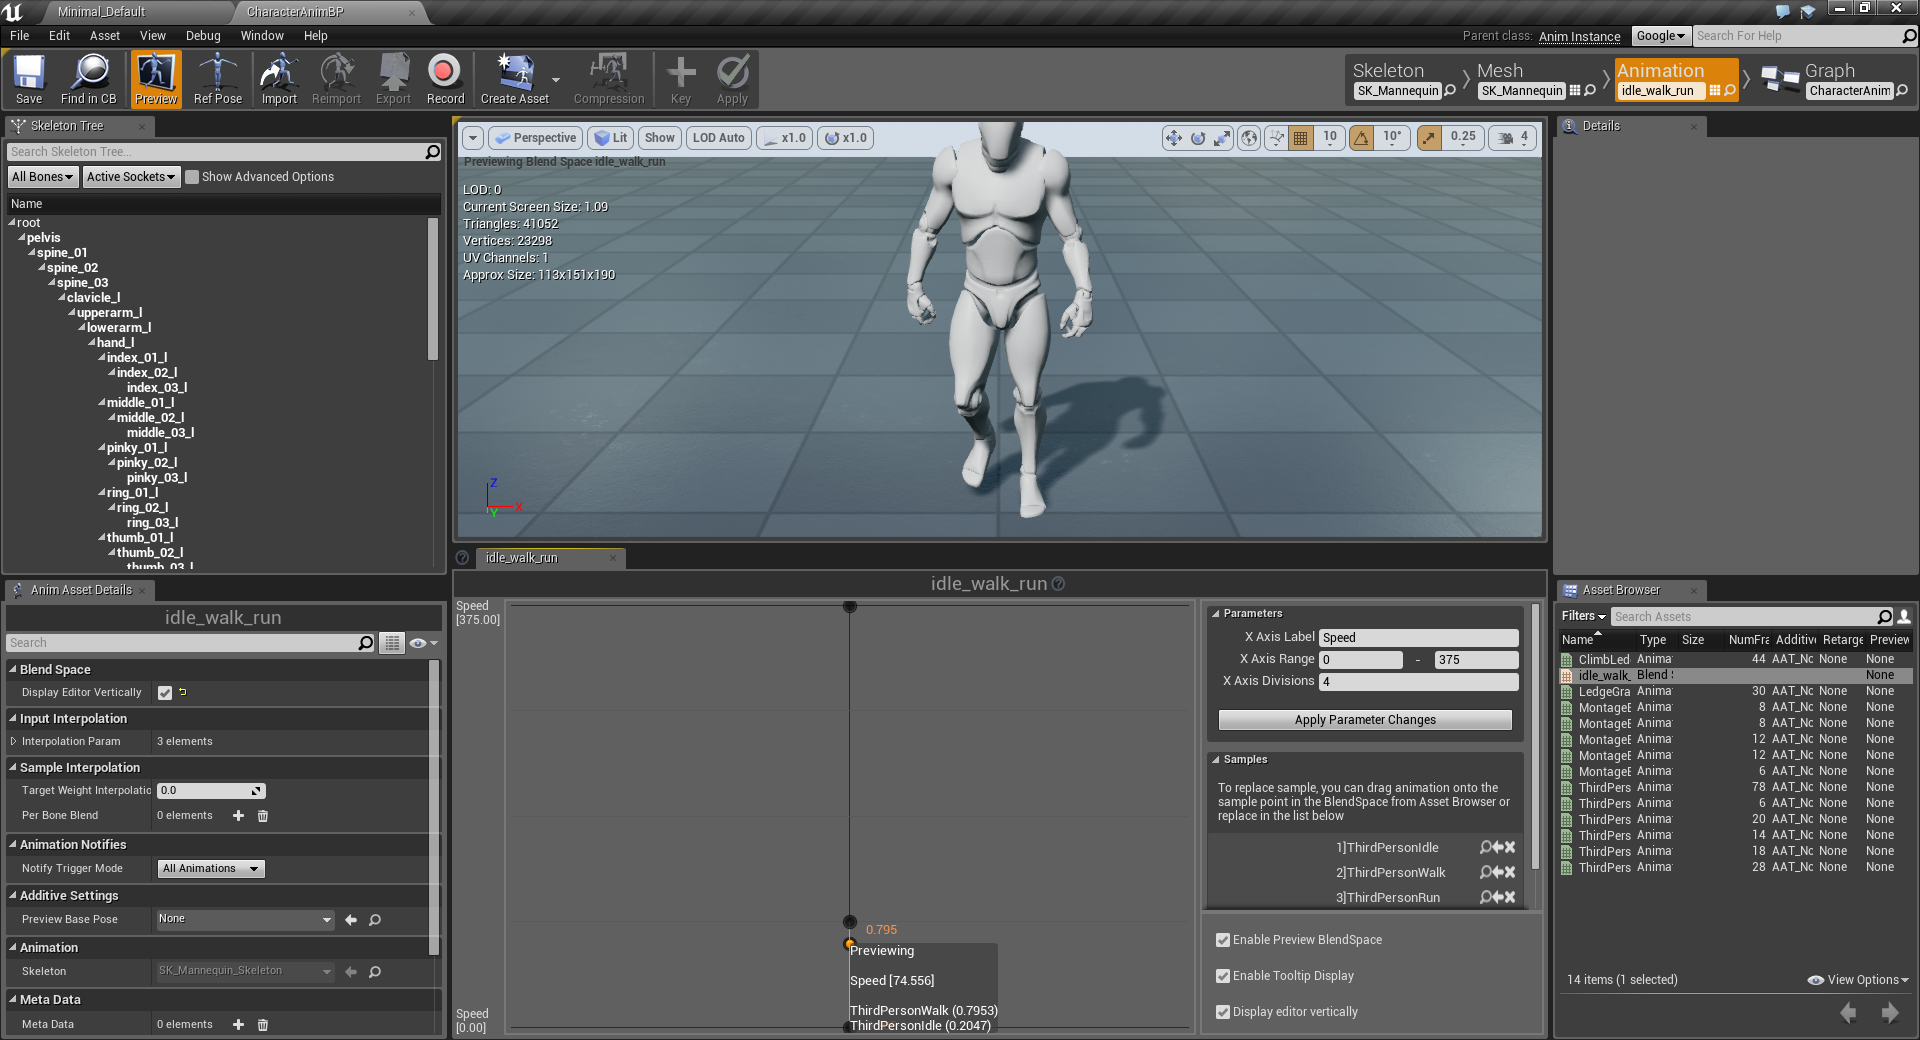
\includegraphics[scale=0.25]{Screeny/Blend_Space}
    \end{center}
    \caption{Podstawy - UE - Blend Spaces}
    \source{Zrzut ekranu z UnrealEngine}
\end{figure}

Warto również wspomnieć o tzw. „Blend Spaces”, czyli możliwość łączenia kilku animacji w jedną. Tej metody używa się, gdy zajdą ustalone okoliczności. Gwarantuje to płynność w przechodzeniu między animacjami. Na przykład, stojąca postać pod wpływem wciśnięcia przycisku zaczyna iść (wartość zmiennej „prędkość” zwiększa się). Jeśli gracz nie puści przycisku, chód zamienia się w bieg.
Aby stworzyć Blend Space, wystarczy kliknąć prawym przyciskiem myszy w przeglądarce plików, w ekranie głównym. Potem z menu kontekstowego wybieramy Animation > Blend Spaces

\newpage
\begin{figure}[!htb]
    \begin{center}
    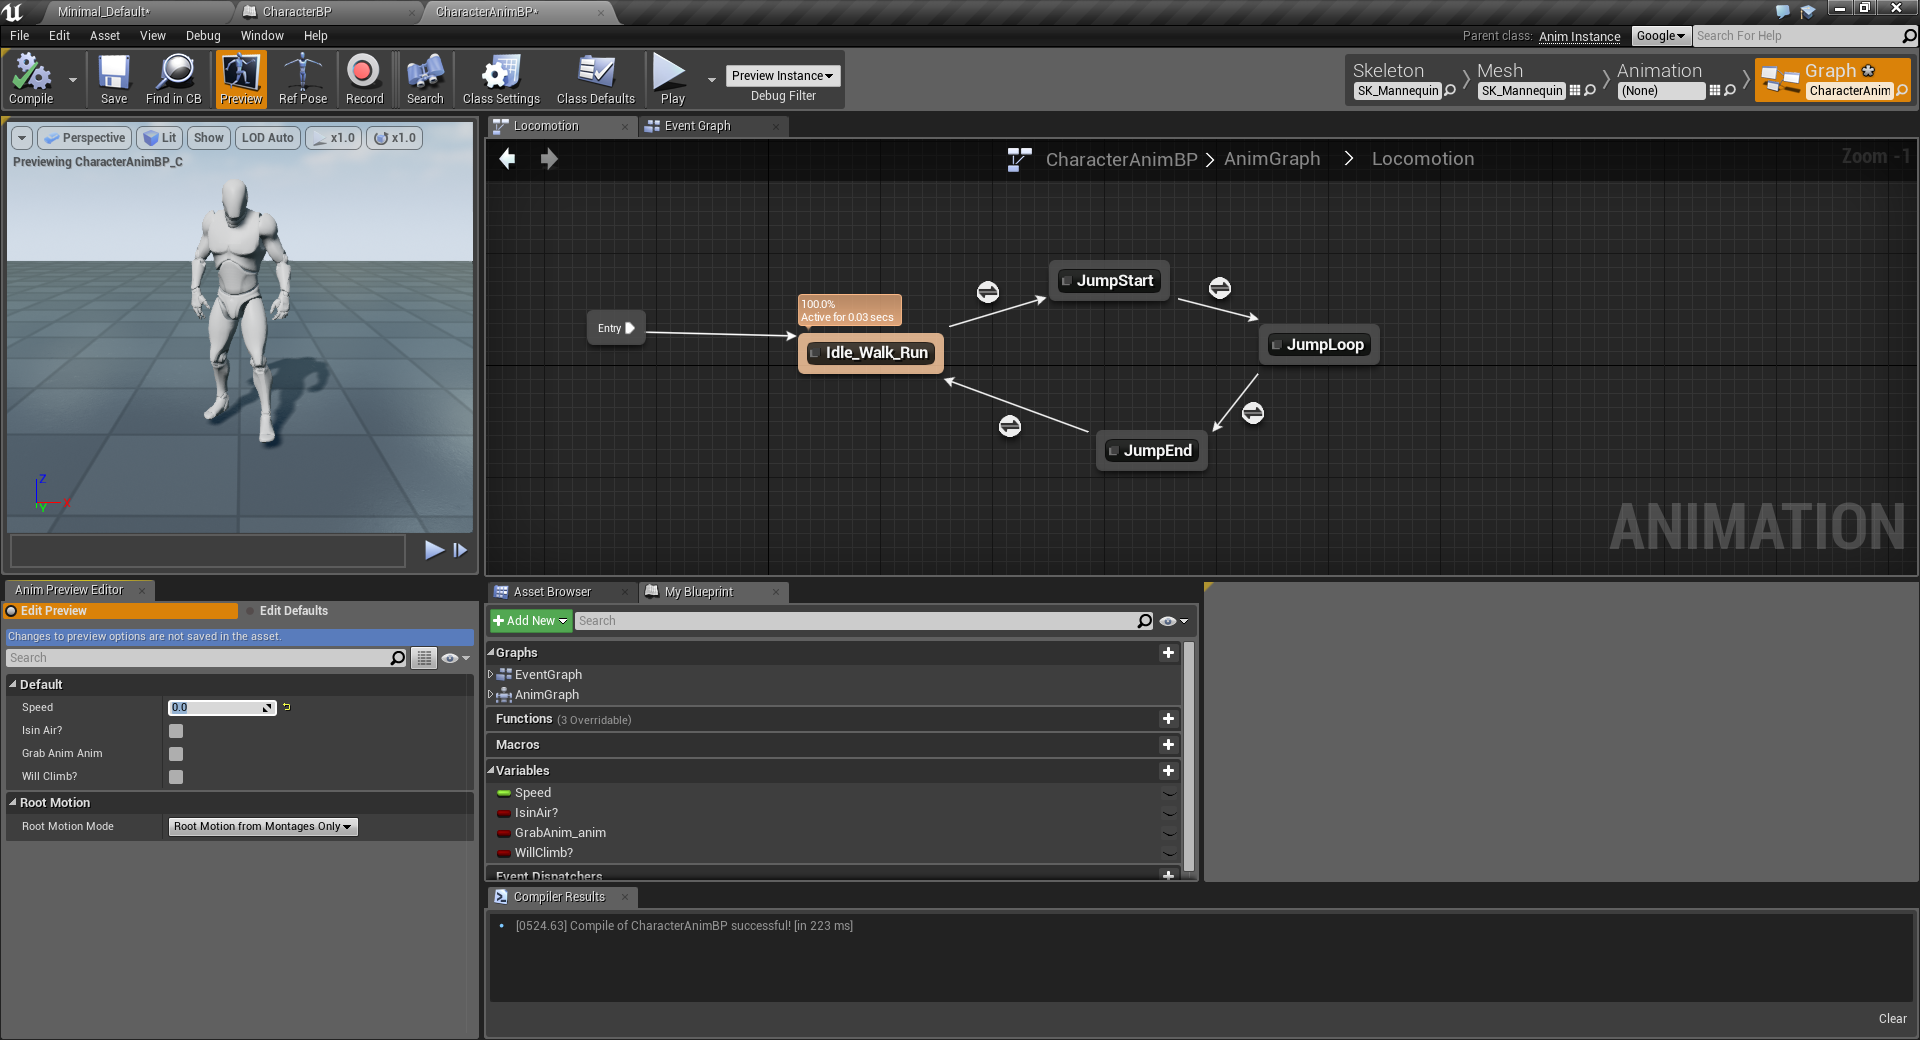
\includegraphics[scale=0.2]{Screeny/AnimGraph_Event}
    \end{center}
    \caption{Podstawy - UE - Graf Animacji}
    \source{Zrzut ekranu z UnrealEngine}
\end{figure}

\begin{figure}[!htb]
    \begin{center}
    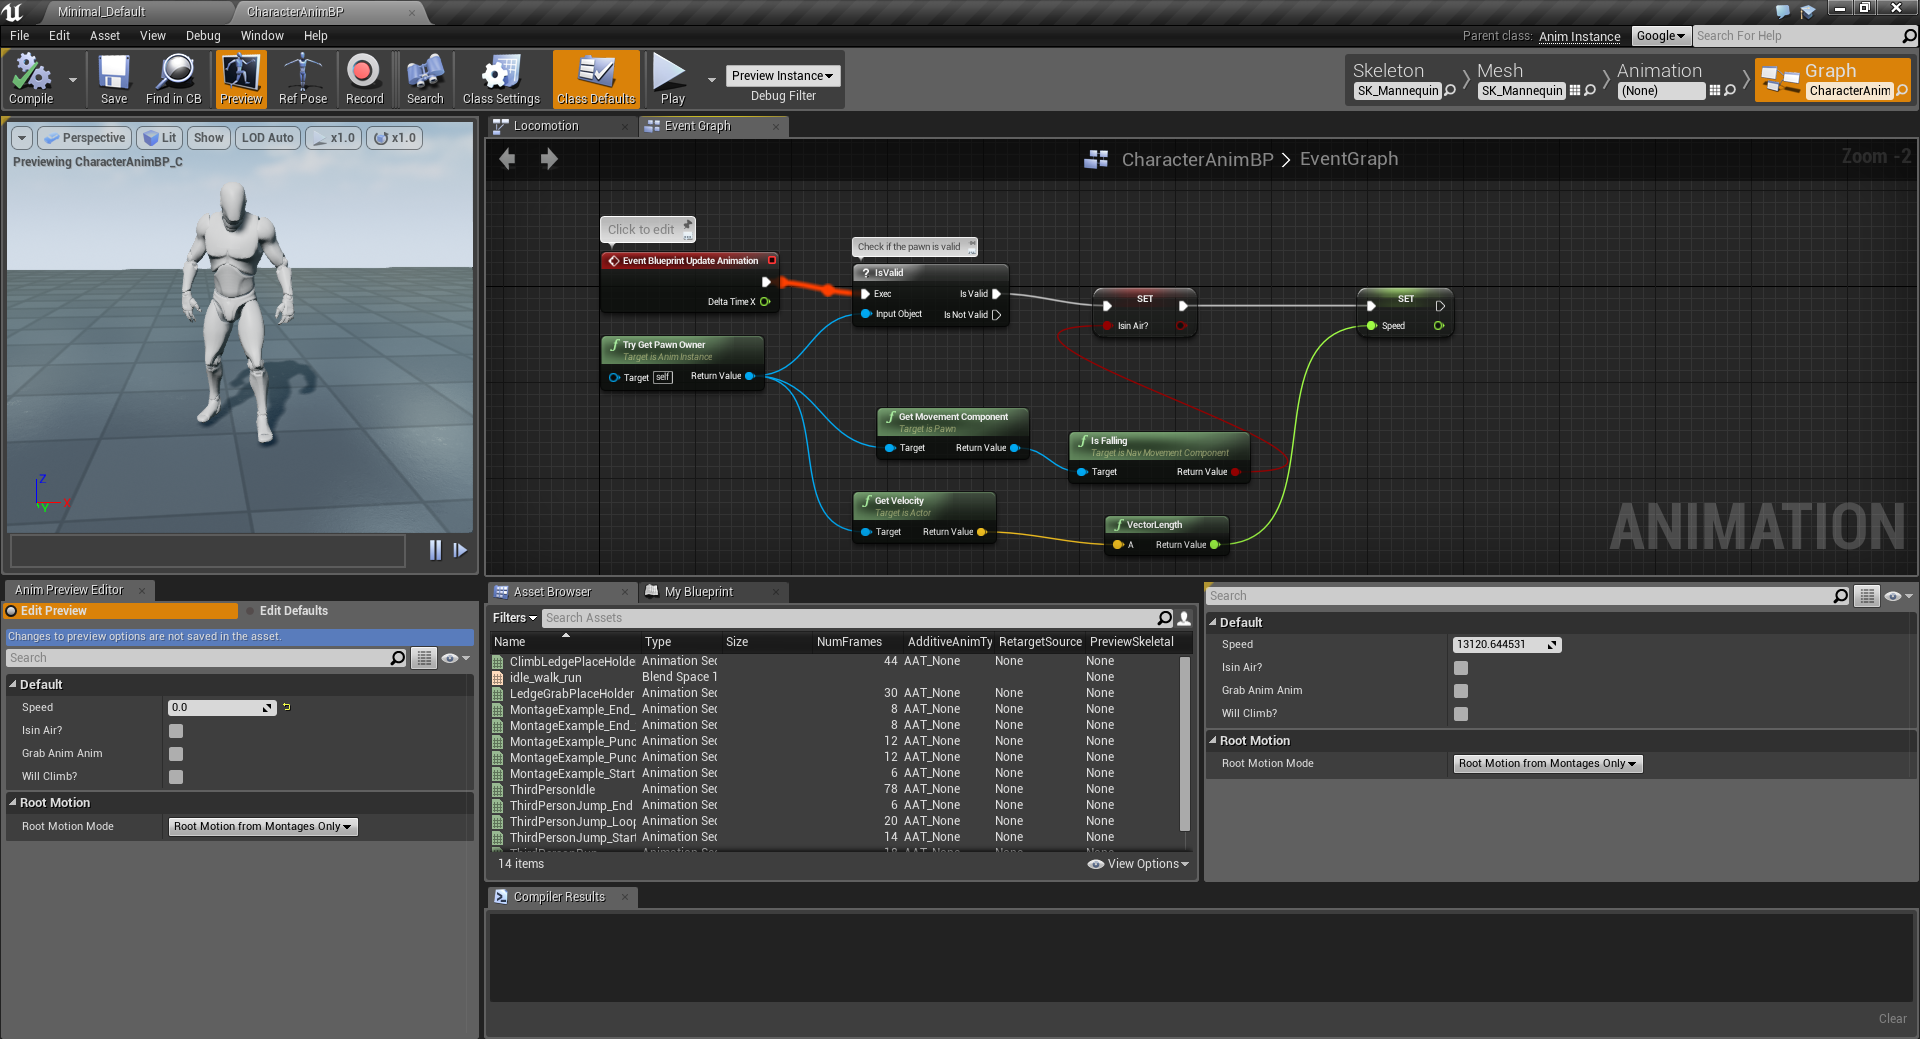
\includegraphics[scale=0.2]{Screeny/EventGraph_Event}
    \end{center}
    \caption{Podstawy - UE - Graf Zdarzeń}
    \source{Zrzut ekranu z UnrealEngine}
\end{figure}

Ostatnią opcją Persony jest ekran grafów. Dzieli się on na dwa ekrany- Graf animacji, oraz graf zdarzeń. Każdy Blueprint związany z animacją posiada oba grafy.
Graf zdarzeń określa wszystkie zdarzenia jakie muszą zajść, aby odtworzona została konkretna animacja w grze. Najczęściej robi się to poprzez modyfikowanie zmiennych zadeklarowanych w grafie. Zmiany zachodzą pod konkretnymi warunkami w grze.

Graf animacji korzysta z grafu zdarzeń, by określić finalną pozę mesh’u w danej klatce. Używa on głównie logiki zawartej w grafie zdarzeń, aby określić czy powinny zajść zmiany. Na przykład, gdy gracz wciska przycisk skoku, wcześniej przygotowany graf zdarzeń może zarejestrować, że powinno to zmienić wartość zmiennej typu bool o nazwie „skok” na True.  Graf animacji rejestruje zmianę i zmienia animację z biegu na skok.

W następnym rozdziale związanym  z Unreal Engine przyjrzymy się bliżej tym systemom i zaprezentujemy je w praktyce.

\chapter{„The Jump" krok po kroku — Unity}

Rozdział ten jest w całości poświęcony opisowi tworzenia jednego konkretnego tytułu przez jedną osobę. Zostały tu zachowane wszystkie ogólne zasady dotyczące tego procesu, trzeba jednak uwzględnić fakt, że w zależności od rodzaju tworzonego tytułu oraz wielkości zespołu przy nim pracującego, konkretne kroki mogą być wykonywane w odmiennej kolejności. Przykładowo, jedna część osób pracujących nad grą może zostać oddelegowana do tworzenia UI, druga do programowania rozgrywki, a jeszcze inna do prac nad obsługą reklam bądź modułu sieciowego. Dopiero w późniejszej fazie produkcji są one łączone w jedną całość.

W przypadku gdy nad grą pracuje jedna osoba, zaleca się aby najpierw implementować podstawowy mechanizm rozgrywki i dopiero w momencie gdy spełni on nasze oczekiwania, kontynuować prace nad pozostałymi częściami gry.

W tej pracy, w fazie planowania zdecydowaliśmy się na stworzenie trójwymiarowej gry z widokiem z trzeciej osoby, z ang. TPP w której biegamy i skaczemy po platformach, z rozgrywką tylko dla jednego gracza. Decyzję taką podjęliśmy z kilku powodów. Oba silniki omawiane w tej pracy dysponują podobnymi narzędziami do obsługi kamery dla tego typu gry. Grę stworzyliśmy w technologii 3D, gdyż zarówno Unity jak i Unreal zostały zaprojektowane właśnie z myślą o trójwymiarowych tytułach. Jednocześnie mogliśmy dostrzec znaczne różnice pomiędzy możliwościami renderowania przez nie grafiki i obsługi fizyki. Dane nam było skorzystać z narzędzi do generowania terenu, popracować nad oświetleniem i zobaczyć jak radzą sobie wbudowane narzędzia do obsługi animacji.

\section{Krok 1 – przygotowanie sceny}


Tworzymy nowy projekt, wybierając opcje 3D i importujemy standardowe assety: Characters i Cameras.

Aby zawczasu zorganizować naszą pracę w oknie Project umieszczamy kilka folderów: Scripts, 3D Assets, Prefabs  i Scenes.

\begin{figure}[!htb]
    \begin{center}
    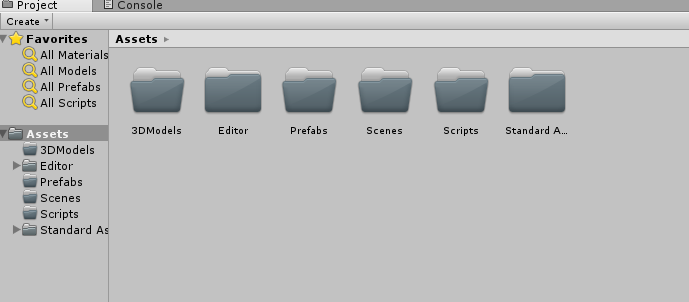
\includegraphics[scale=0.25]{Screeny/UnityKrokPoKroku/foldery}
    \end{center}
    \caption{Krok po kroku - Unity - Foldery}
Jeśli odpowiednio zaimportowaliśmy podstawowe assety, dodatkowo pojawią nam się foldery Editor i Standard Assets.
    \source{Zrzut ekranu z Unity}
\end{figure}

Dodajemy poziom gry na której toczyć się będzie akcja, poprzez wybranie File $\rightarrow$ New Scene w pasku menu i umieszczamy ją w folderze Scenes. Otwieramy tę scenę klikając na nią dwukrotnie w oknie projektu.

W zależności od użyej wersji Unity, na nowej scenie może brakować światła, dodajemy je z paska menu GameObject $\rightarrow$ Light $\rightarrow$ Directional Light.

Teraz tworzymy nowy teren, klikamy GameObject w pasku menu i wybieramy 3D Object $\rightarrow$ Terrain, nazywamy go Ground i umieszczamy w folderze 3D Assets.

Jeśli nie posiadamy domyślnych tekstur terenu możemy je pobrać z Asset Store. Z paska menu wybieramy Window $\rightarrow$ Asset Store. Następnie wyszukujemy interesujące nas tekstury i importujemy je do Unity. W tym projekcie skorzystaliśmy z darmowej paczki Forest Grounds Texture Pack. Tekstury terenu możemy stworzyć też sami przy pomocy zewnętrznego programu graficznego. Teksturę dodajemy zaznaczając obiekt Terrain $\rightarrow$ klikamy ikonkę pędzla we właściwościach komponentu $\rightarrow$ Edit Textures. Jeśli chcemy aby nasz teren składał się z różnych tekstur, ponownie doddajemy teksturę i przy pomocy pędzla „malujemy” podłoże.

Podstawą naszej postaci będzie przykładowy model który zaimportowaliśmy przy tworzeniu nowego projektu. Znajduje się on w folderze Standard Assets $\rightarrow$ ThirdPersonCharacter $\rightarrow$ Prefabs $\rightarrow$ ThirdPersonController.

Obiekt ten jest tzw. Prefabem. Prefaby są to obiekty gry z rozszerzeniem .prefab w naszym projekcie. W odróznieniu od zwykłych obiektów pozwalaja one na modyfikowanie ich kopii  z poziomu jednego prefaba, bez konieczności edycji każdego obiektu oddzielnie. Oznacza to, że jeśli umieścimy wiele kopii tego samego przeciwnika w wielu miejscach, to jeśli będzie on prefabem, modyfikując wartości jednego z nich równocześnie wprowadzimy zmiany dla pozostałych kopii.

\begin{figure}[!htb]
    \begin{center}
    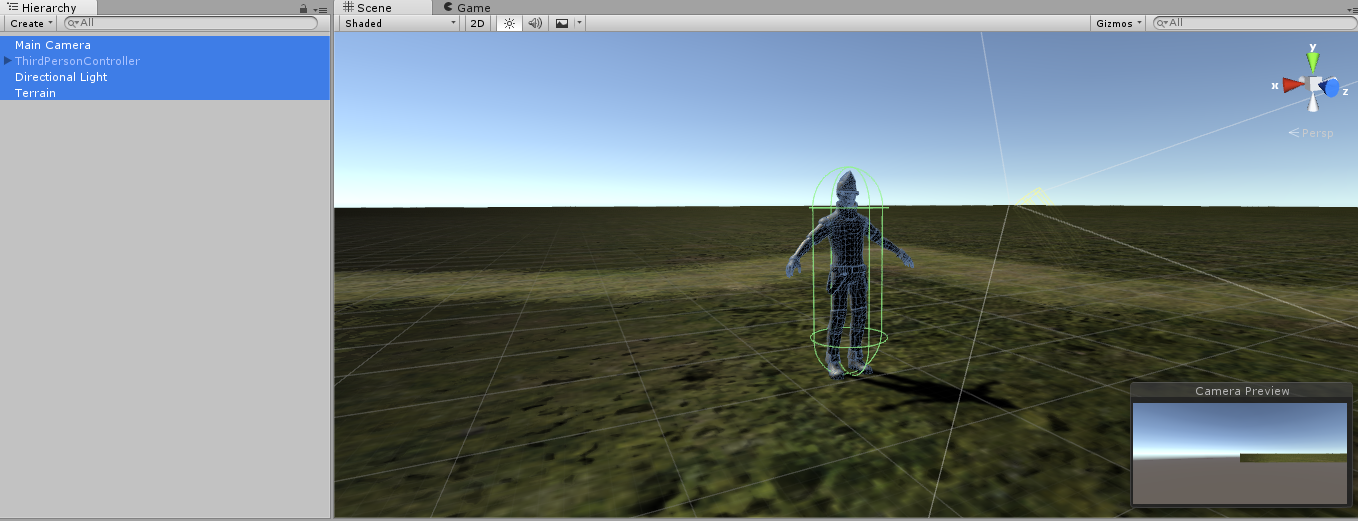
\includegraphics[scale=0.25]{Screeny/UnityKrokPoKroku/krok1_endscreen.png}
    \end{center}
    \caption{Krok po kroku - Unity - Scena}
Zaznaczone elementy wystarczą by zbudować i przetestować podstawową mechanikę naszej gry: kamerę TPP oraz poruszanie postaci.
    \source{Zrzut ekranu z Unity}
\end{figure}

\section{Krok 2 – obsługa podstawowych mechanik}

Do podstawowych mechanik rozgrywki, tzw. Core  Mechanics, zaliczane są wszystkie podstawowe czynności które będą wielokrotnie wykonywane przez gracza w przeciągu całej gry. W zależności od typu gry mogą się one znacząco od siebie różnić, i tak dla dwuwymiarowej gry platformowej podstawową mechaniką jest m.in. skakanie, w grach typu FPS jest to strzelanie, a dla gry przygodowej zbieranie przedmiotów i interakcja z otoczeniem.

Niezależnie do rodzaju tworzonej gry do podstawowych mechanik zawsze zalicza się obsługa kamery oraz sterowanie. Stworzenie sprawnie operującej dynamicznej kamery może okazać się dużym wyzwaniem. Sterowanie zaś musi być płynne i responsywne.

W przypadku tworzonej przez nas gry, Unity zapewnia nam rozwiązania dla obu tych mechanik. Użyty przez nas w  poprzednim kroku model postaci, posiada już dwa komponenty, odpowiedzialne za poruszanie się i obsługę sterowania naszej postaci: Third Person User Control oraz Third Person Character. Dodatkowo możemy zauważyć komponent Animator, odpowiedzialny za wszystkie animacje naszego obiektu, oraz Rigidbody, który jest niezbędny do działania powyższych komponentów. Dzięki niemu, oraz komponentowi Capsule Collider, nasza postać może także poruszać się po utworzonym przez nas terenie.

Jesteśmy już w stanie poruszać naszym obiektem jednak po odpaleniu gry przyciskiem Play nie jesteśmy w stanie niczego dostrzec. Wynika to z faktu, że nasza kamera wyświetla tę część sceny, która aktualnie jest pusta.

Kamera jest jednym z najważniejszych środków przy budowaniu dynamiki gry. Statyczna kamera znajduje swoje zastosowanie jedynie przy prostych grach 2D, np. popularnych na urządzeniach mobilnych grach typu One Touch, gdzie obsługujemy sterowanie tylko pojedynczymi tapnięciami. W tego typu grach to Game Objecty są poruszane tak by wchodziły/wychodziły z pola widzenia kamery. Zdecydowana większość gier skupia się jednak na odpowiednich ujęciach i pracy kamery, aby – podobnie jak w filmach – przedstawiać graczowi najważniejsze wydarzenia.

I w tym wypadku Unity wychodzi nam naprzeciw, dostarczając prefaby obsługujące pracę kamery. Podobnie jak w wypadku naszego modelu, przy tworzeniu projektu zaimportowaliśmy odpowiednie assety. Aby umieścić nową kamerę na scenie przenosimy na nią prefab FreeLookCameraRig znajdujacy się w Standard Assets $\rightarrow$ Cameras $\rightarrow$ Prefabs. Aby kamera zaczęła śledzić naszego gracza, po kliknięciu go na scenie, w oknie inspektora zmieniamy Tag, na „Player”. Ustawiamy kamerę możliwie blisko modelu, kopiując jego zawartość Transform do prefaba naszej kamery (robimy to klikając prawym przyciskiem myszki na nazwie komponentu i wybieramy opcję „Copy Component”, następnie w docelowym komponencie wybieramy opcę „Paste Component Values”).

Zarówno obiekt ThirdPersonController (zmieńmy jego nazwę na Player) jak i FreeLookCameraRig (nazwijmy go TPPCamera), dają nam do dyspozycji różne opcje, umożliwiające dostosowanie sterowania i pracy kamery do naszych potrzeb. Jeśli chcemy jedynie poeksperymentować z różnymi ustawieniami, warto robić to po wciśnięciu przycisku Play. Wszystkie zmiany dokonane podczas działania gry będą natychmiast widoczne, jednak zostaną cofnięte po jej wyłączeniu.

\section{Krok 3 - Cele gry}

Możemy już biegać i skakać naszą postacią, a także swobodnie rozglądać się przy pomocy kamery. Cele gry powinny zostać uprzednio zdefiniowane w GDD, szczególnie jeśli do ich osiągnięcia niezbędna jest implementacja odpowiednich mechanik. Najprostszym podejściem jest ustalenie warunków wygranej i przegranej, oraz danie graczowi jasno do zrozumienia na jakich zasadach się one opierają.

W naszej grze, aby odnieść sukces, gracz będzie musiał odnaleźć i dotrzeć do specyficznego punktu na mapie, sygnalizowanego przez czerwony słup dymu.

Warunkiem przegranej będzie śmierć gracza. Gracz umrzeć będzie mógł na dwa sposoby: upadając z dużej wysokości lub wpadając do wody.

Aby móc testować mechanizm śmierci podczas upadku, dodajemy do gry przykładowe wzniesienie. Klikamy na obiekt Terrain i wybieramy pierwszą opcje od lewej. Służy ona do tworzenia wzniesień na naszym terenie. Tworzymy wolno wznoszące się wzniesienie na które może wbiec gracz, punkt szczytowy powinien wynieść co najmniej czterokrotność wysokości gracza. Następnie tworzymy skrypt WinLoseCondition i podpinamy go do obiektu Player:

\begin{lstlisting}

using UnityEngine;
using System.Collections;

public class WinLoseCondition : MonoBehaviour {
    Rigidbody rb;
    Animator anim;
    // Use this for initialization
    void Start ()
    {
        rb = gameObject.GetComponent<Rigidbody> ();
        anim = gameObject.GetComponent<Animator> ();
    }

    void OnCollisionEnter (Collision other)
    {
        if (other.gameObject.tag == „Water") {
            Death ();

        }
        if (rb.velocity.y < -10) {
            if (other.gameObject.tag == „Ground") {
                Death ();
            }
        }
        if (other.gameObject.tag == „Finish") {
            Win ();

        }
    }

}

\end{lstlisting}

W powyższym kodzie tworzymy prywatne zmienne rb i anim. Następnie korzystamy z funkcji GetComponent. Służy ona do uzyskiwania dostepu do komponentów wybranego przez nas GameObjectu. GameObject pisany z małej litery oznacza w tym wypadku obiekt do którego ten skrypt jest podpięty. Możemy w tym miejscu umieścić dowolną zmienną typu GameObject, należy jednak zwrócić uwagę na to, czy obiekt ten posiada komponent do którego próbujemy się dostać. Jeśli odwołamy się do nieistniejącego komponentu to wartość zmiennej będzie równa null. Wszelkie późniejsze odwołanie do niej spowoduje zawieszenie bądź wywalenie się gry. Najprostszym sposobem unikania tego problemów jest stawianie flagi, sprawdzającej czy wykorzystywana wartość jest różna od null.

Funkcja OnCollisionEnter wykonuje się za każdym razem gdy kolider obiektu do którego podpięliśmy skrypt, zetknie się z innym koliderem. Pierwszy warunek sprawdza, czy tag obiektu, do którego należy kolider z którym się zetknęliśmy, nazywa się „Water”. Jeśli tak to nastąpi śmierć gracza. Drugi warunek sprawdza aktualną prędkość poruszania się naszej postaci w pozycji wertykalnej. Jeśli jest ona odpowiednio wysoka (wartość ujemna oznacza, że nasza postać porusza się z góry do dołu, z im większej wysokości spadamy, tym bardziej wzrasta prędkość zgodnie z wartością przyspieszenia ziemskiego) w momencie zderzenia z ziemią gracz umrze. Ostatni warunek sprawdza czy dotarliśmy do punktu oznaczonego tagiem Finish, który oznacza naszą wygraną.

Chcemy aby w momencie śmierci bohatera odtwarzana była odpowiednia animacja, a po chwili następował restart gry. Nasza postać nie posiada animacji śmierci, możemy jednak bez problemu wyszukać gotowe animacje oparte na humanoidalnym szkielecie w Asset Store. Ułatwieniem dla nas będzie jeśli uda nam się znaleźć animację w formacie .fbx. Aby dodać nową animację dla postaci, musi otworzyć okno animatora. Robimy to klikając dwukrotnie na obiekt animatora znajdujący się w Standard Assets $\rightarrow$ ThirdPersonCharacter $\rightarrow$ Animator. Po otwarciu animatora zobaczymy siatkę na której umieszczono animacje. Strzałki pomiędzy nimi oznaczają przejścia w animacji. Przenosimy nasz plik .fbx z animacją do animatora i zmieńmy jego nazwę na Death. Dzięki temu będziemy w stanie odwołać się do niej z komponentu Animator naszego obiektu.
W naszym projekcie wykorzystaliśmy paczkę Huge Mockap Library do pobrania za darmo z Asset Store.

Do naszego skryptu dodajemy poniższe funkcje :

\begin{lstlisting}

void Death ()
    {
        anim.Play („Death");
        Invoke ("Restart", 2f);

        Debug.Log („Nie żyjesz");
    }

    void Win ()
    {
        Invoke („Restart", 2f);
        Debug.Log („Wygrałeś");
    }

    void Restart ()
    {
        Application.LoadLevel (Application.loadedLevelName);
    }

\end{lstlisting}

W funkcji Death() najpierw wywołujemy animację, którą właśnie dodaliśmy.
Funkcja Invoke służy do opóźniania wywołania funkcji. W tym wypadku po dwóch sekundach wywołamy funkcję Restart, która załaduje aktualna scenę na nowo.

\section{Krok 4 – Interfejs użytkownika}

Kolejnym ważnym aspektem gry jest to jak „rozmawiamy” z graczem. Do komunikacji wykorzystujemy przede wszystkim wydarzenia w świecie gry, oraz tzw. UI – user interface.

UI służy do obsługi i wyświetlania opcji gry dostępnych graczowi, informowania o aktualnym celach i stanie rozgrywki. Wydarzenia w świecie gry mogą spełniać podobną rolę, jednak nie muszą one mieć konkretnego wpływu na przebieg rozgrywki, elementy UI zaś powinny zawsze oferować jakąś funkcjonalność.

Aby stworzyć podstawowe UI w Unity, z pasku menu wybieramy opcję GameObject $\rightarrow$ UI $\rightarrow$ Button. W oknie hierarchii pojawią się nam dwa nowe obiekty: Canvas, będący tłem dla wszystkich  elementów UI, oraz EventSystem odpowiedzialny m.in. za obsługę przycisków. Wewnątrz obiektu Canvas znajdziemy obiekt o nazwie Button – zduplikujmy go. Rozstawiamy nasze przyciski na scenie, oraz zmieniamy ich nazwy na Play oraz Exit. Po odpaleniu gry zauważymy, że niezależnie od pozycji naszej kamery, oba przyciski znajdują się na pierwszym planie.

\newpage
\begin{figure}[!htb]
    \begin{center}
    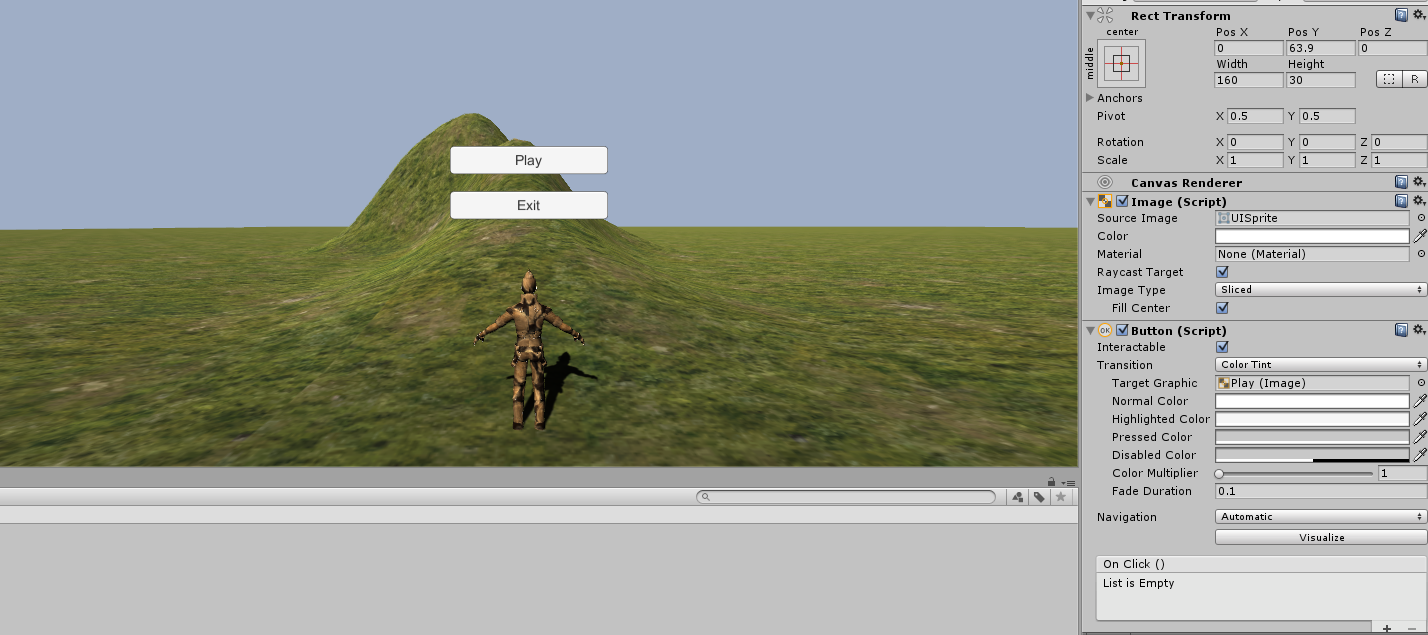
\includegraphics[scale=0.25]{Screeny/UnityKrokPoKroku/krok4_buttony.png}
    \end{center}
    \caption{Krok po kroku - Unity - Przyciski}
Możemy dowolnie przekształcać rozmiar oraz wygląd przycisków utworzonych przy pomocy unitowego UI. Służą do tego komponenty RectT Transform, Image oraz Button.
    \source{Zrzut ekranu z Unity}
\end{figure}

Aby nasze przyciski zaczęły coś robić musimy stworzyć skrypt obsługujący ich działanie, nazwijmy go UIController:

\begin{lstlisting}

using UnityEngine;
using System.Collections;

public class UIController : MonoBehaviour {
    public GameObject Canvas;
    public GameObject Player;
    public GameObject Camera;


    public void PlayButton() {
        Canvas.SetActive (false);
        Player.GetComponent<UnityStandardAssets.Characters
	.ThirdPerson.ThirdPersonUserControl> ().enabled = true;
        Camera.GetComponent<UnityStandardAssets.Cameras
			.FreeLookCam> ().enabled = true;
    }

    public void ExitButton() {
        Application.Quit ();
    }
}

\end{lstlisting}

Dodajemy pusty obiekt UI Controll do naszej sceny, i podpinamy do niej powyższy skrypt. Następnie zaznaczamy stworzone przez nas wcześniej przyciski. Używamy znaku plusa na dole komponentu Button i przenosimy do niego obiekt UI Controll. Dzięki temu uzyskamy dostęp do wszystkich publicznych funkcji skryptu UI Controll. Dla przycisku Play zaznaczamy funkcję PlayButton(), a dla przycisku Exit – ExitButton().

Funkcja PlayButton() wyłącza Canvas, oraz włącza komponenty ThirdPersonUserControl i FreeLookCam. Funkcja ExitButton zamyka naszą aplikację.

Tworząc obiekt UI typu Text możemy dodatkowo umieścić nazwę naszej gry jako element Canvasu.

Czerwony dym widoczny w naszej grze także pełni rolę UI – wskazuje nam gdzie znajduje się nasz cel na mapie. Tego typu informacje zaliczamy do wydarzeń w świecie gry.

\section{Krok 5 – Kreacja świata gry}

W tym momencie nasza gra znajduje się już w stadium grywalności, można więc rozpocząć prace nad stworzeniem odpowiedniego otoczenia. Wszystkie zaprogramowane funkcje i stworzone assety są w tym etapie łączone ze sobą w jedną całość.

Nasz gracz jest  w stanie zginąć spadając z wysokości lub wpadając do wody. Ustawiamy w naszej grze kilka wzniesień. Możemy do tego użyć naszego obiektu Terrain lub wyszukać odpowiednie assety w Asset Storze.

Domyślna woda Unity dostępna jest tylko w płatnej wersji. Wodę w grze dodaliśmy korzystając z odpowiedniej paczki pobranej ze strony.

\href{http://forum.unity3d.com/threads/riverwater-the-free-epic-water-solution-for-unity-free-users.235860/}{http://forum.unity3d.com/threads/riverwater-the-free-epic-water-solution-for-unity-free-users.235860/}

Korzystając z zakładki Lighting możemy odpowiednio modyfikować kolor i natężenie swiatła naszego otoczenia lub dodać mgłę.

Dodatkowo wykorzystaliśmy na scenie tzw. Skybox. Jest to asset służący do tworzenia złudzenia realistycznego nieba. Skybox otacza całą scenę dając złudzenie złożonej przestrzeni ponad horyzontem. Możemy go ustawić w tej samej zakładce co światło otoczenia i mgłę.

\begin{figure}[!htb]
    \begin{center}
    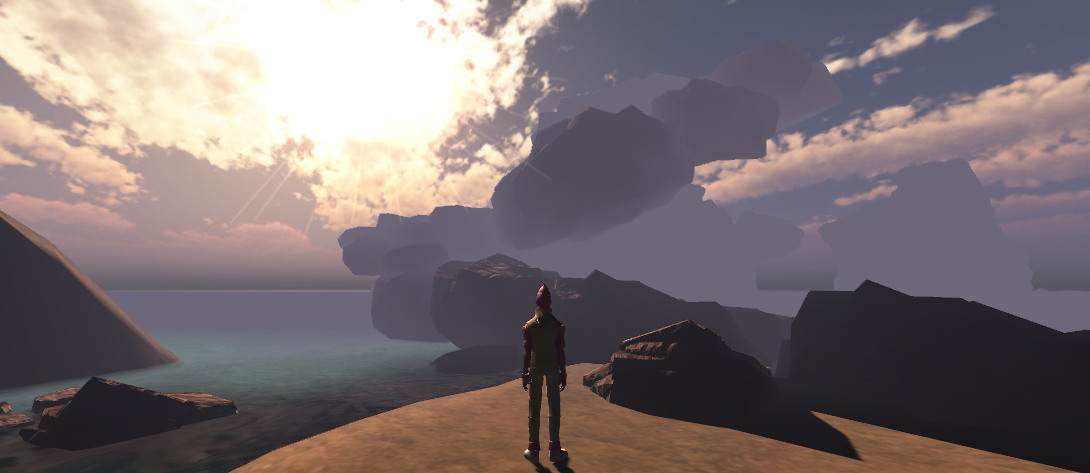
\includegraphics[scale=0.25]{Screeny/UnityKrokPoKroku/gotowa_gra.png}
    \end{center}
    \caption{Krok po kroku - Unity - Gotowa gra}
Przykładowy screen z gry po dodaniu Skyboxa, mgły i zmianie koloru światła na cieplejszy.
    \source{Zrzut ekranu z Unity}
\end{figure}

Jeśli chcemy dodatkowo upiększyć nasza grę, w Asset Storze możemy znaleźć mnóstwo darmowych modeli 3D, generatorów otoczenia oraz efektów specjalnych, które niejednokrotnie są importowane z przykładowymi scenami, pozwalającymi nam podejrzeć ich działanie.

Teraz gdy nasza gra jest gotowa, powinniśmy zbudować ją na wybrane urządzenie i przetestować jej działanie. W zależności od wybranej platformy, gotowy plik może wymagać kompilacji w dodatkowych programach dostarczanych przez producentów danej platformy np. Xcode dla IOS -a i AppleTV, lub Android Studio dla urządzeń z systemem Android.

PC, Linux i Mac nie wymagają dodatkowego oprogramowania. Aby zbudować grę na te urządzenia wybieramy z paska menu File $\rightarrow$ Build Setting. W zakładce Player Settings możemy m.in. zmienić tytuł naszej gry lub sposób jej wyświetlania, dodać ikonki i splashe. Następnie zaznaczamy naszą platformę i klikamy przycisk build. Pozostaje nam czekać, aż gra się skompiluje.

\chapter{„The Jump" krok po kroku — Unreal Engine}

\begin{figure}[!htb]
    \begin{center}
    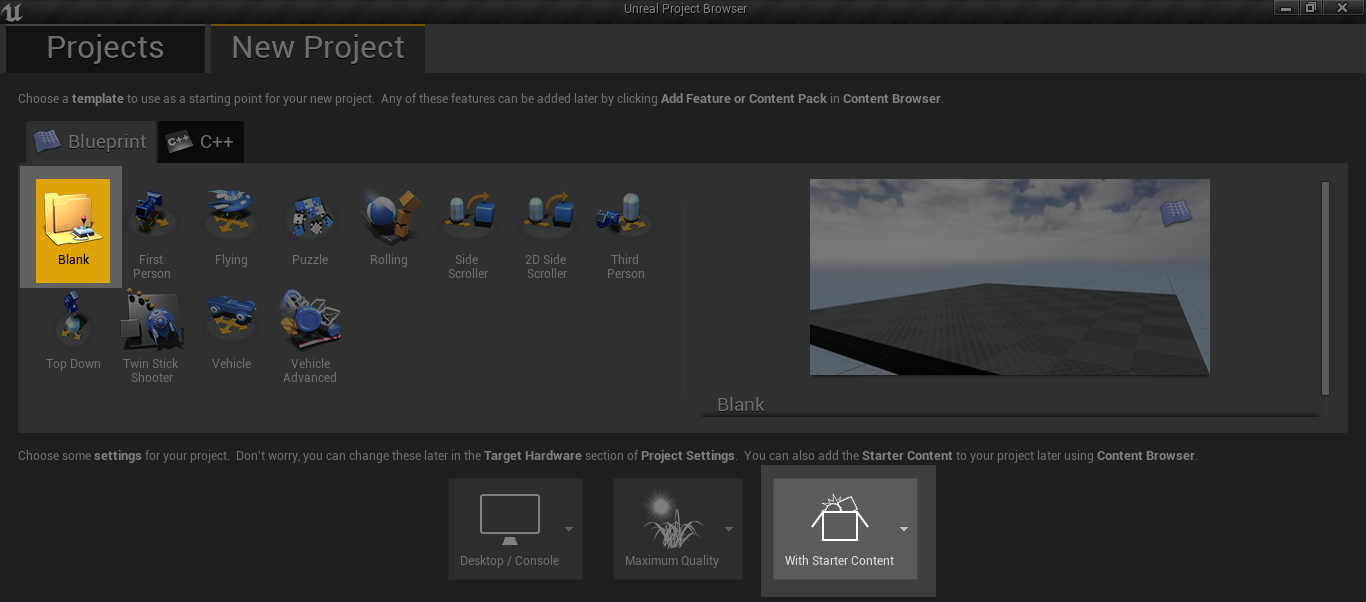
\includegraphics[scale=0.35]{Screeny/UeKrokPoKroku/UE-Climb-NewProject.png}
    \end{center}
    \caption{Krok po kroku - UE - Ekran główny}
    \source{Zrzut ekranu z UnrealEngine}
\end{figure}

W tym rozdziale prześledzimy proces tworzenia prostej gry w Unreal Engine przy pomocy blueprintów. Projekt tworzymy od podstaw. W tym celu na ekranie startowym wybieramy z dostępnych opcji projektu „Blank”. Jeżeli nie chcemy ręcznie pobierać assetów czy materiałów warto upewnić się, że zaznaczona została opcja „with starter content”. W projekcie będziemy również korzystać z modelu i animacji postaci (dostępne na stronie \url{https://wiki.unrealengine.com/File:ThirdPerson_FBX.zip}) oraz z animacji chwytania krawędzi i wspinaczki (dostępne na stronie \url{https://www.crocopede.com/free-stuff}), które już na początku pracy z projektem warto zaimportować.

\section{Krok 1 - Import postaci i ustawianie klawiszy wejściowych}

Aby zaimportować modele i animacje do projektu wystarczy rozpakować pobrane paczki w dowolnym miejscu na komputerze. Następnie należy przeciągnąć rozpakowane pliki do przeglądarki zawartości w edytorze Unreal Engine. Podczas importowania animacji edytor będzie wymagał od nas wskazania dla niej szkieletu. Warto więc jako pierwszy plik zaimportować „SK\_Maneqquin\_skeleton”, który go zawiera. Po zaimportowaniutego pliku możemy już grupowo dodać resztę animacji. Warto w tym momencie wprowadzić pewien porządek i utworzyć kilka katalogów – główny dla postaci, a w nim zagnieżdżony dla animacji.

Po zaimportowaniu wszystkich plików możemy ustawić klawisze wejściowe. Dzięki temu gra zostanie poinformowana, że wciśnięcie danego klawisza ma wywołać akcję. Aby to zrobić, z lewego górnego rogu edytora wybieramy zakładkę „Edit”, a następnie wybieramy opcję „Project settings...”. W nowootwartym oknie, na liście po lewej stronie, w sekcji „Engine” wyszukujemy i wybieramy „Input”. W zakładce „bindings" dodajemy i ustawiamy odpowiednie klawisze tak jak na obrazku poniżej.

\newpage
\begin{figure}[!htb]
    \begin{center}
    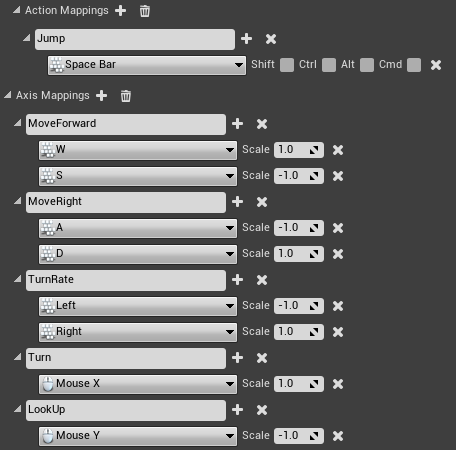
\includegraphics[scale=0.75]{Screeny/UeKrokPoKroku/UE-Inputs.png}
    \end{center}
    \caption{Krok po kroku - UE - Klawisze wejściowe}
     Możemy przydzielić dowolne klawisze do danej akcji, jednakże powyższe przyjęły się jako domyślne w grach.
    \source{Zrzut ekranu z UnrealEngine}
\end{figure}

\newpage
\section{Krok 2 - Graf animacji i graf zdarzeń}

\begin{figure}[!htb]
    \begin{center}
    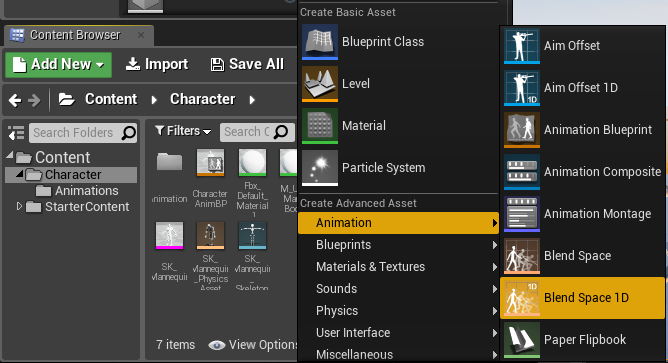
\includegraphics[scale=0.5]{Screeny/UeKrokPoKroku/UE-BlendSpace-Add.png}
    \end{center}
    \caption{Krok po kroku - UE - Blend Spaces - Tworzenie}
    \source{Zrzut ekranu z UnrealEngine}
\end{figure}

Samo dodanie klawiszy wejściowych nie wystarczy aby móc sterować naszą postacią. Program już wie na jakie przyciski ma reagować, nie wie natomiast co ma z nimi zrobić. W tym przypadku przydadzą się nam graf animacji i graf zdarzeń.

Zanim jednak do nich przejdziemy, stworzymy przejście dla naszej animacji. Aby to zrobić w przeglądarce zawartości, w katalogu „Character” klikamy „Add New”, a następnie z zakładki „Animation” wybieramy „Blend Space 1D”. Zaznaczamy szkielet naszej postaci i po wciśnięciu przycisku „ok” nazywamy nasz nowopowstały plik „Idle\_Walk\_Run”.

Aby go otworzyć klikamy na niego dwukrotnie lewym przyciskiem myszy. Dla naszej wygody możemy zaznaczyć opcję „Display editor vertically” w środkowym dolnym panelu.

W parametrach w „X Axis Range” drugą liczbę zmieniamy na 375. To od niej zależy szybkość zmiany z jednej animacji na drugą. Następnie klikamy „Apply Parameter Changes”, aby zaktualizować panel po lewej stronie. Aby dodać animacje na osi wystarczy ją przeciągnąć z menu assetów. W tym przypadku dodajemy trzy - „Idle” na samym dole, „Walk” nieco wyżej, oraz „Run” na samej górze. Zapisujemy plik i z niego wychodzimy.

\begin{figure}[!htb]
    \begin{center}
    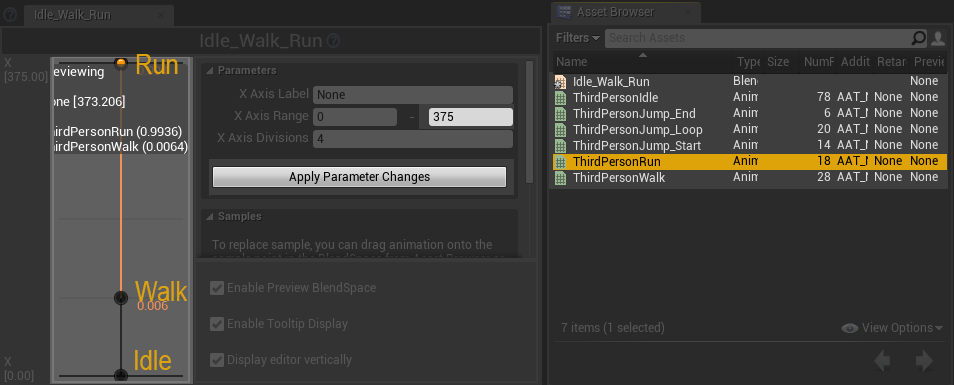
\includegraphics[scale=0.5]{Screeny/UeKrokPoKroku/UE-BlendSpace-IdleWalkRun.png}
    \end{center}
    \caption{Krok po kroku - UE - Blend Spaces - Idle Walk Run}
    \source{Zrzut ekranu z UnrealEngine}
\end{figure}

Następnie stworzymy nowy plan animacji w przeglądarce zawartości. Aby to zrobić klikamy przycisk „Add New” w momencie, w którym znajdujemy się w katalogu „Character”. Z listy wybieramy „Animation”, a następnie „Animation Blueprint”.

\begin{figure}[!htb]
    \begin{center}
    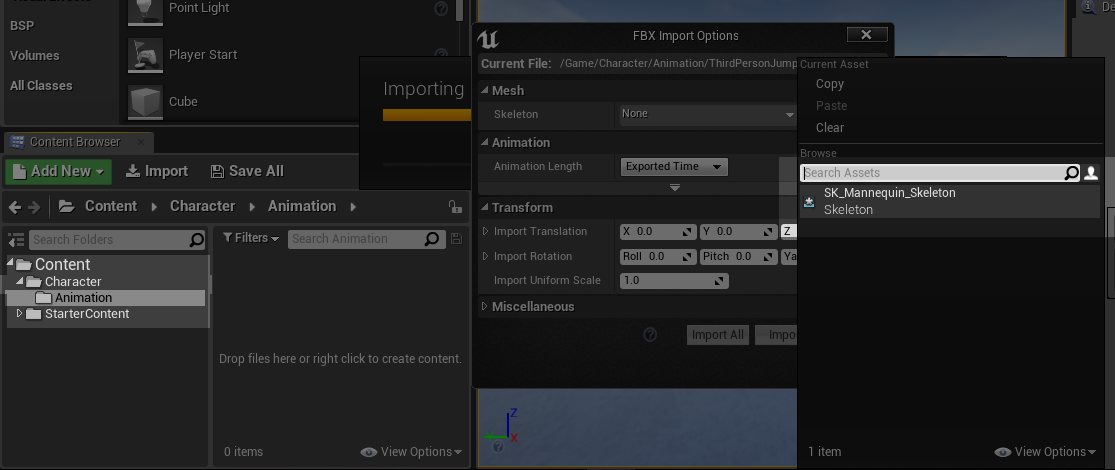
\includegraphics[scale=0.35]{Screeny/UeKrokPoKroku/UE-Import.png}
    \end{center}
    \caption{Krok po kroku - UE - Importowanie}
    \source{Zrzut ekranu z UnrealEngine}
\end{figure}

\newpage
W nowootwartym okienku mamy dwa pola wyboru. W klasie rodzicielskiej wybieramy „AnimInstance”. O ile nie tworzymy gry z pojazdami będzie to najczęściej używana przez nas klasa. W drugim polu upewniamy się, że został wybrany szkielet naszej postaci i klikamy przycisk „ok”. Nowopowstały plik możemy nazwać „CharacterAnimBP”. W menu konstektowym klikamy na niego dwukrotnie.

\begin{figure}[!htb]
    \begin{center}
    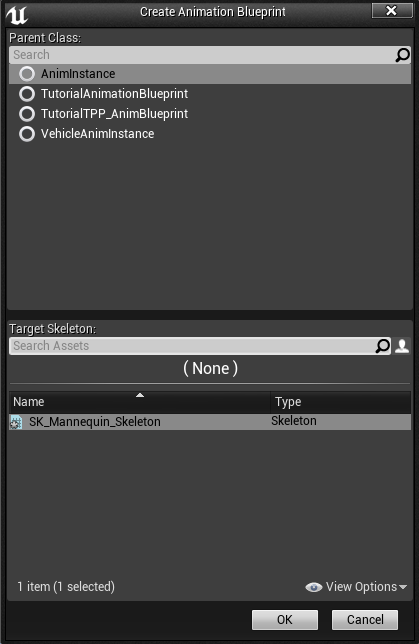
\includegraphics[scale=0.75]{Screeny/UeKrokPoKroku/UE-AnimBPcreate.png}
    \end{center}
    \caption{Krok po kroku - UE - Animation Blueprint - tworzenie}
    \source{Zrzut ekranu z UnrealEngine}
\end{figure}

\newpage
\subsection{Graf Animacji}
Pierwsze co musimy zrobić to dodać maszynę stanów. W tym celu możemy poprowadzić linię od „Result” w „Final Animation Pose”, a następnie wyszukać i wybrać „Add New State Machine...”. Możemy nazwać ją „Locomotion” i kliknąć na nią dwukrotnie lewym przyciskiem myszy.

W tym miejscu będziemy tworzyć stany i ich połączenia. Aby stworzyć pierwszy stan przeciągamy linię od „entry”, a następnie wybieramy „Add state...”. Nazywamy go „Idle\_Walk\_Run” i klikamy na niego dwukrotnie.

Do grafu z przeglądarki assetów dodajmy stworzone przez nas wcześniej przejście „Idle\_Walk\_Run” i łączymy je z „Final Animation Pose”.  Nie chcemy, aby prędkość animacji była stała, dlatego klikamy prawym przyciskiem na zielonym kółeczko w „Idle\_Walk\_Run” i wybieramy „Promote to Variable”. Naszą zmienną nazywamy „Speed”.

\begin{figure}[!htb]
    \begin{center}
    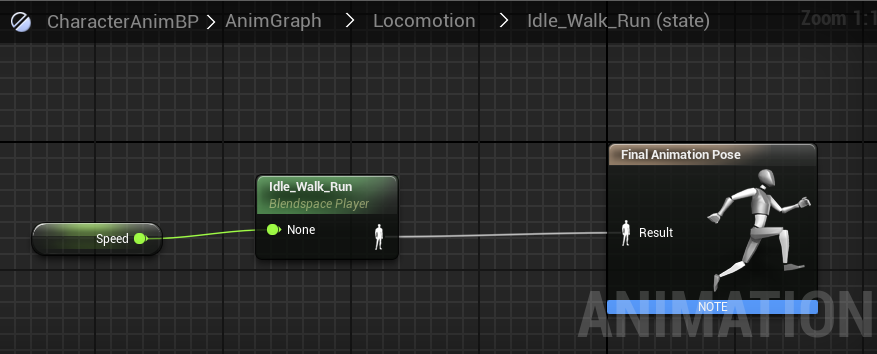
\includegraphics[scale=0.6]{Screeny/UeKrokPoKroku/UE-AnimGraph-IdleWalkRun.png}
    \end{center}
    \caption{Krok po kroku - UE - Graf Animacji - Idle Walk Run}
    \source{Zrzut ekranu z UnrealEngine}
\end{figure}

\newpage
Następnie dodajemy stany dla skoku. Jeden dla stanu początkowego, drugi dla zapętlonej animacji skoku, a ostatni dla stanu końcowego. Łączymy je tak jak na poniższym rysunku. Następnie wchodzimy w każdy z nich po kolei i z przeglądarki assetów przyłączamy odpowiednią animację.

\begin{figure}[!htb]
    \begin{center}
    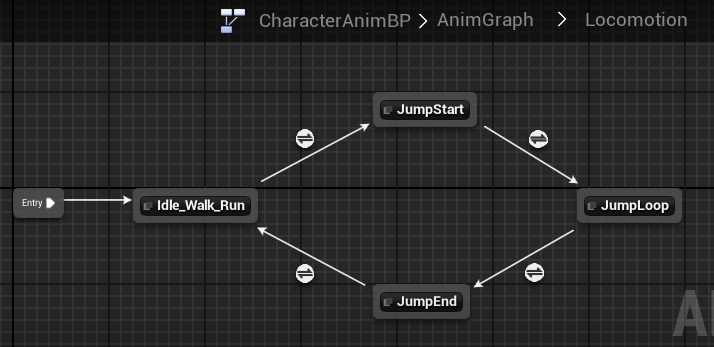
\includegraphics[scale=0.6]{Screeny/UeKrokPoKroku/UE-AnimGraph-Anim.png}
    \end{center}
    \caption{Krok po kroku - UE -  Graf Animacji - dodanie skoku}
    \source{Zrzut ekranu z UnrealEngine}
\end{figure}

Połączenia pomiędzy stanami również musimy zedytować. Zaczynamy od połączenia „Idle\_Walk\_Run” z „JumpStart”. Aby je zedytować dwukrotnie klikamy kółeczko obok strzałki. W tym miejscu tworzymy zmienną, która będzie nas informowała czy postać jest w powietrzu. W tym celu klikamy prawym przyciskiem myszy na czerwone kółko w „Result” i wybieramy „Promote to Variable”. Nazywamy naszą zmienną „IsInAir?”. Kolejne połączenia zedytujmy według poniższego schematu.
\newpage
\begin{figure}[!htb]
    \begin{center}
    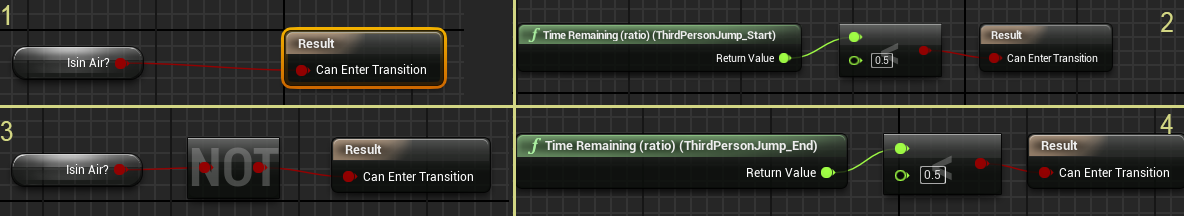
\includegraphics[scale=0.5]{Screeny/UeKrokPoKroku/UE-AnimGraph-Connect.png}
    \end{center}
    \caption{Krok po kroku - UE -  Graf Animacji - Połączenia stanów}
 (1) połączęnie „Idle\_Walk\_Run” z „JumpStart”, (2) połączenie „JumpStart” z „JumpLoop”, (3) połączenie „JumpLoop” z „JumpEnd”, (4) połączenie „JumpEnd” z „Idle\_Walk\_Run”
    \source{Zrzut ekranu z UnrealEngine}
\end{figure}

\subsection{Graf Zdarzeń}
Przechodzimy do grafu zdarzeń. Pierwsze co w musimy zrobić, to sprawdzić, czy w ogóle istnieje gracz. Jeżeli nie, żaden kod się nie wykona. Jeżeli jednak istnieje będziemy mogli wykonywać dalsze czynności.

\begin{figure}[!htb]
    \begin{center}
    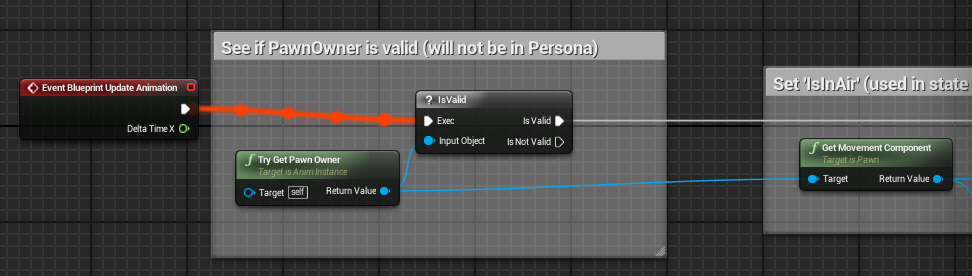
\includegraphics[scale=0.6]{Screeny/UeKrokPoKroku/UE-EventGraph-IsValid.png}
    \end{center}
    \caption{Krok po kroku - UE -  Graf Zdarzeń - Walidacja postaci}
    \source{Zrzut ekranu z UnrealEngine}
\end{figure}

Następnie sprawdzamy czy postać jest w powietrzu. Możemy to zrobić pobierając pozycję naszej postaci, oraz wykorzystując wbudowane funkcje „IsFalling” i „IsFlynig”.

\begin{figure}[!htb]
    \begin{center}
    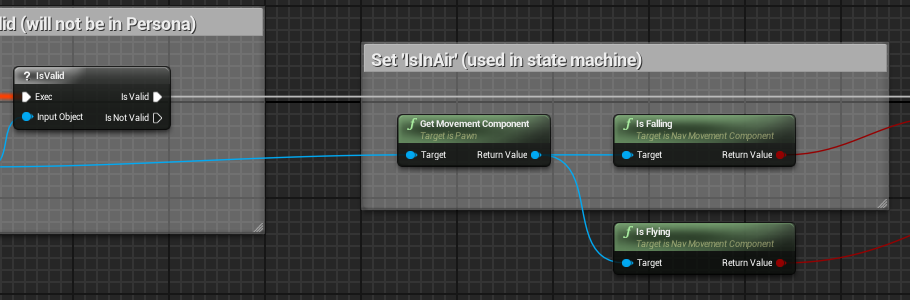
\includegraphics[scale=0.6]{Screeny/UeKrokPoKroku/UE-EventGraph-IsInAir.png}
    \end{center}
    \caption{Krok po kroku - UE -  Graf Zdarzeń - Czy w powietrzu?}
    \source{Zrzut ekranu z UnrealEngine}
\end{figure}

Widząc czy nasza postać się unosi, spada, lub nie zmienia swojego położenia możemy odpowiednio ustalić wartość zmiennej „IsInAir?”.

\begin{figure}[!htb]
    \begin{center}
    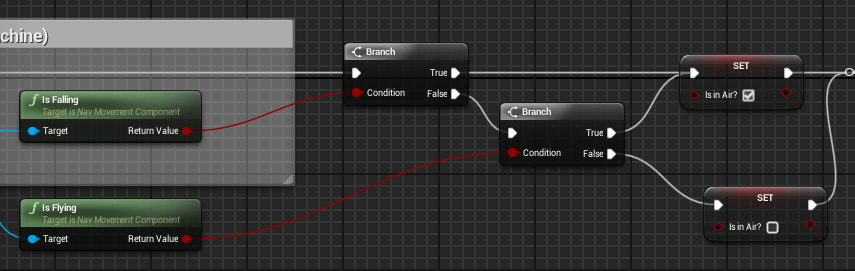
\includegraphics[scale=0.6]{Screeny/UeKrokPoKroku/UE-EventGraph-SetIsInAir.png}
    \end{center}
    \caption{Krok po kroku - UE -  Graf Zdarzeń - Ustawianie zmiennej "IsInAir?"}
    \source{Zrzut ekranu z UnrealEngine}
\end{figure}

\newpage
Na koniec pozostaje nam tylko ustawienie prędokści naszej animacji.

\begin{figure}[!htb]
    \begin{center}
    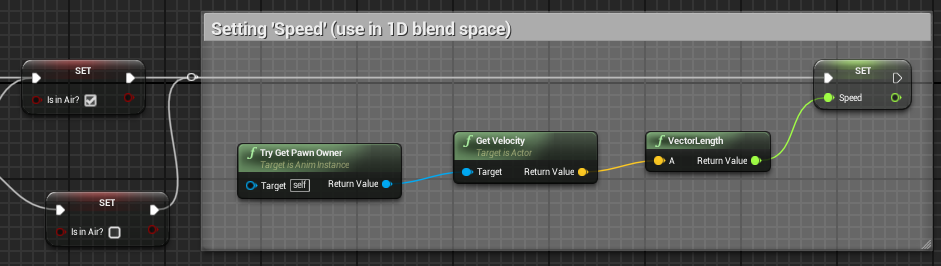
\includegraphics[scale=0.6]{Screeny/UeKrokPoKroku/UE-EventGraph-Speed.png}
    \end{center}
    \caption{Krok po kroku - UE -  Graf Zdarzeń - Ustawianie prędkości}
    \source{Zrzut ekranu z UnrealEngine}
\end{figure}

\section{Krok 3 - Postać i scena}

Na początku musimy stworzyć blueprint naszej postaci. W tym celu w katalogu „Character” klikamy „Add New” i wybieramy „Blueprint Class”. Z dostępnych opcji wybieramy „Character”, nowopowstały plik nazywamy „CharacterBP”, a następnie otwieramy go.

W komponentach po lewej stronie nowootwartego okna zaznaczamy „Mesh” i przenosimy swoją uwagę na prawą stronę edytora. W tym miejscu zmieniamy dwie rzeczy. Pierwszą z nich w zakładce „Mesh” jest szkielet. Zmieniamy go na ten, który posiadamy. W głównym oknie dostosowujemy go do strefy kolizji, t.j. obniżamy go, oraz obkręcamy o 90 stopni przeciwnie do ruchów wskazówek zegara. Następnie po prawej stronie wyszukujemy zakładkę „Animation” i w „Anim Blueprint Generated Class” zmieniamy na wcześniej utworzony „CharacterAnimBP”.

\newpage
\begin{figure}[!htb]
    \begin{center}
    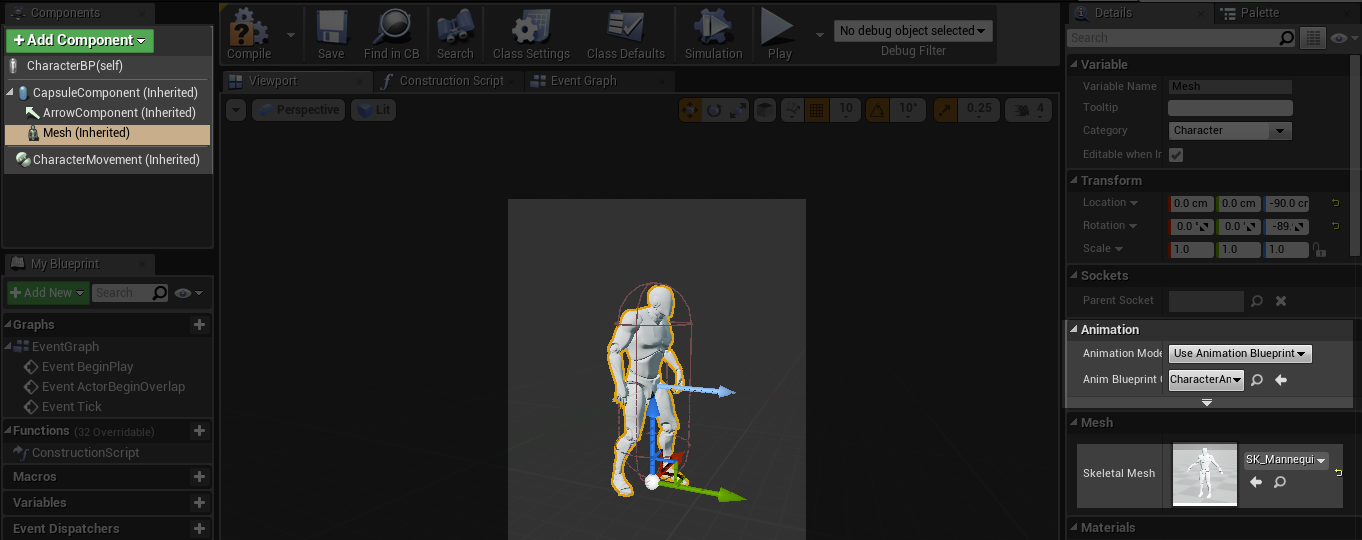
\includegraphics[scale=0.35]{Screeny/UeKrokPoKroku/UE-CharacterBP-Viewport.png}
    \end{center}
    \caption{Krok po kroku - UE -  CharacterBP - Viewport}
    \source{Zrzut ekranu z UnrealEngine}
\end{figure}


Wracamy do komponentów. Tam wyszukujemy i dodajemy „SpringArm”, a następnie zmieniamy jego nazwę na „CameraBoom”. Klikamy na nią, a następnie w panelu po prawej stronie wyszukujemy „Camera Settings” i zaznaczamy w niej „Use Pawn Control Rotation”. Dzięki temu kamera po napotkaniu kolizji przybliży się do postaci. Jest to przydatne w momencie, w którym gracz pokieruje postać do zamkniętego pomieszczenia. 

Następnie w menu komponentów dodajmy samą kamerę, a następnie przeciągamy ją na „CameraBoom”. Możemy dostosować jej pozycję jakkolwiek chcemy.

\begin{figure}[!htb]
    \begin{center}
    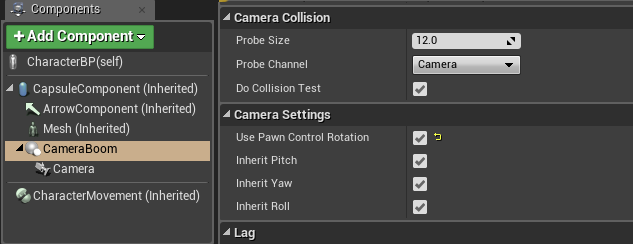
\includegraphics[scale=0.35]{Screeny/UeKrokPoKroku/UE-CharacterBP-Camera.png}
    \end{center}
    \caption{Krok po kroku - UE -  CharacterBP - Kamera}
    \source{Zrzut ekranu z UnrealEngine}
\end{figure}

\newpage
W menu komponentów wybieramy „CharacterBP” i odznaczmy w nim „Use Controller Rotation Yaw”. Następnie przejdźmy do komponentu „CharacterMocement” i w panelu po prawej stronie w „General Settings” wyszukujemy i zaznaczamy „Orient Rotation to Movement”.

Następnie przechodzimy do zakładki „Event Graph”. To tutaj będziemy przekazywali postaci co ma robić po wciśnięciu konkretnego przycisku. Zaczynamy od poruszania się. Musimy pobrać pozycje postaci, rozbić ją na wektory, które po wciśnięciu odpowiedniego klawisza będą się zmieniać.

\begin{figure}[!htb]
    \begin{center}
    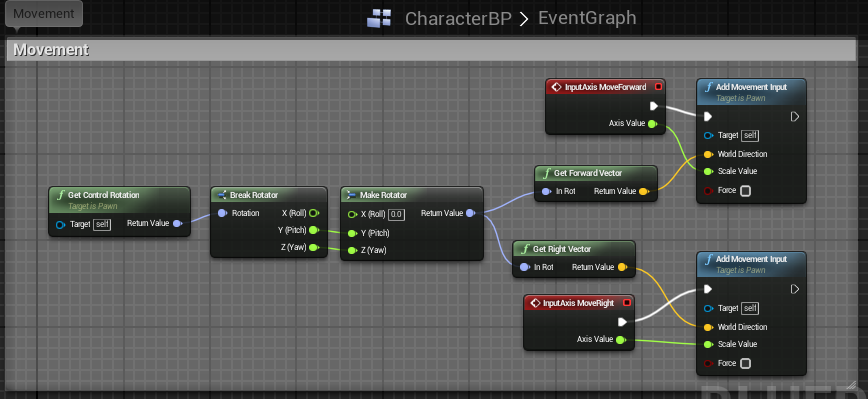
\includegraphics[scale=0.35]{Screeny/UeKrokPoKroku/UE-CharacterBP-Movement.png}
    \end{center}
    \caption{Krok po kroku - UE -  CharacterBP - Poruszanie}
    \source{Zrzut ekranu z UnrealEngine}
\end{figure}

Kolejnym krokiem będzie ustawienie akcji dla myszy i skoku.

\begin{figure}[!htb]
    \begin{center}
    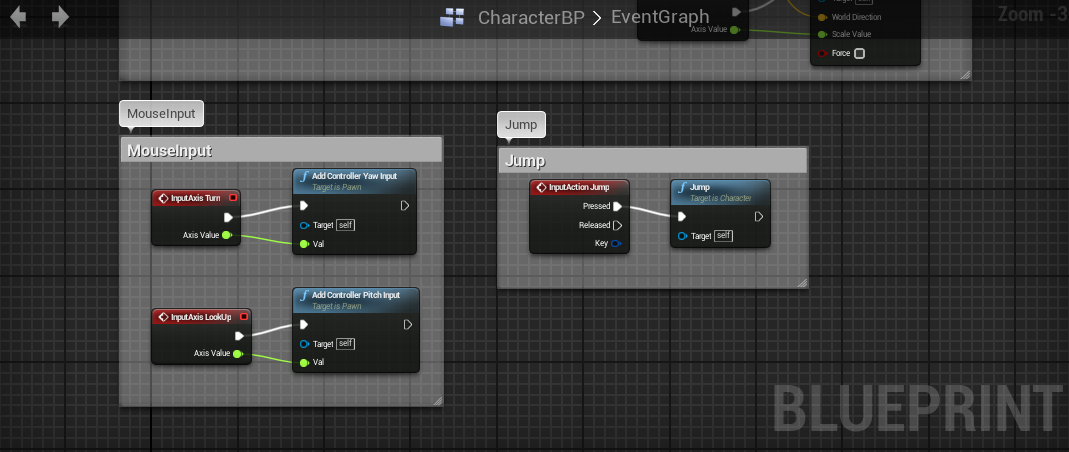
\includegraphics[scale=0.35]{Screeny/UeKrokPoKroku/UE-CharacterBP-MouseAndJump.png}
    \end{center}
    \caption{Krok po kroku - UE -  CharacterBP - Mysz i Skok}
    \source{Zrzut ekranu z UnrealEngine}
\end{figure}

\newpage
Przechodzimy do głównego okna projektu. Tam w przeglądarce zawartości w katalogu „Character” tworzymy nowy „Blueprint Class”. Z dostępnych opcji wybieramy „GameMode” i nowopowstały plik nazywamy „MyGame”. Otwieramy go klikając na niego dwukrotnie lewym przyciskiem myszy.

W panelu po prawej stronie, w sekcji „Classes” w „Default Pawn Class” ustawiamy „CharacterBP”.

\begin{figure}[!htb]
    \begin{center}
    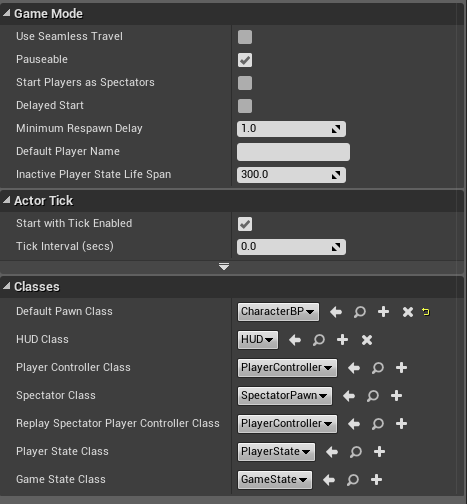
\includegraphics[scale=0.35]{Screeny/UeKrokPoKroku/UE-MyGame-Class.png}
    \end{center}
    \caption{Krok po kroku - UE -  MyGame - Domyślna klasa postaci}
    \source{Zrzut ekranu z UnrealEngine}
\end{figure}

\newpage
Aby ustawić tryb gry dla danej sceny najpierw wracamy do głównego okna projektu. Z panelu nad podglądem sceny wybieramy „Settings”, a następnie „World Setting”. Pojawi nam się nowa zakładka w panelu po prawej stronie. W sekcji „GameMode” w „GameMode Override” zmieniamy na „MyGame”.

\begin{figure}[!htb]
    \begin{center}
    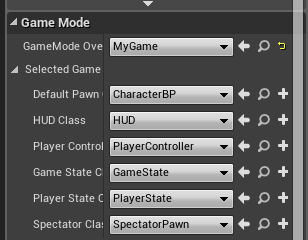
\includegraphics[scale=0.35]{Screeny/UeKrokPoKroku/UE-MyGame-WorldSetting.png}
    \end{center}
    \caption{Krok po kroku - UE -  MyGame - Ustawienia poziomu}
    \source{Zrzut ekranu z UnrealEngine}
\end{figure}

Jest to jednak rozwiązanie tylko lokalne. Aby każda nowa scena w tym projekcie również posiadała te same ustawienia trybu gry, należy przejść do „Project settings”. Z panelu po lewej w noowootwartym oknie wybieramy „Maps \& Modes” i w sekcji „Default Modes” zmieniamy „Default GameMode” na „MyGame”.

\begin{figure}[!htb]
    \begin{center}
    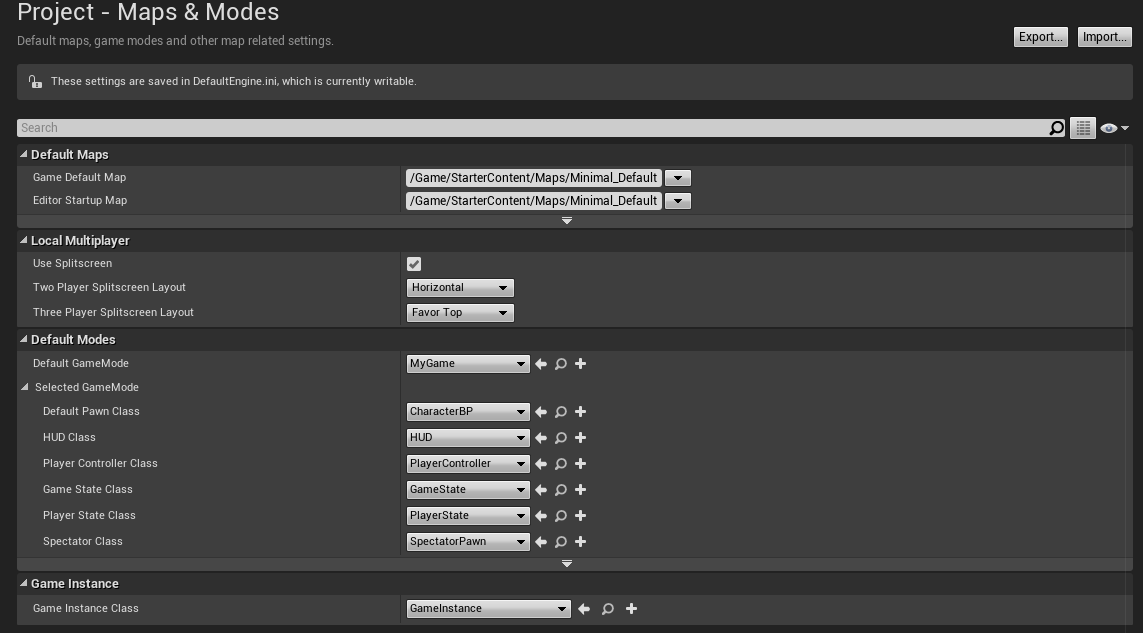
\includegraphics[scale=0.35]{Screeny/UeKrokPoKroku/UE-MyGame-ProjectSettings.png}
    \end{center}
    \caption{Krok po kroku - UE -  MyGame - Ustawienia projektu}
    \source{Zrzut ekranu z UnrealEngine}
\end{figure}

Ze sceny usuwamy domyślną kapsułę z graczem. Na jej miejsce przeciągamy z przeglądarki zawartości „CharacterBP”, dzięki czemu będziemy widzieć naszą postać. Musimy jednak powiedzieć jeszcze programowi, aby to właśnie ją przydzielił graczowi do kontrolowania. W tym celu mając ją zaznaczoną po prawej stronie wyszukujemy „Auto Possess Player” w zakładce „Pawn”, a następnie zmieniamy ją na „Player 0”.

\begin{figure}[!htb]
    \begin{center}
    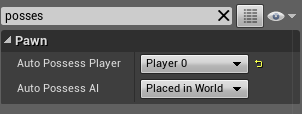
\includegraphics[scale=0.35]{Screeny/UeKrokPoKroku/UE-MyGame-Posses.png}
    \end{center}
    \caption{Krok po kroku - UE -  MyGame - Posses}
    \source{Zrzut ekranu z UnrealEngine}
\end{figure}

Teraz możemy zedytować istniejącą scenę. Możemy usunąć, zmienić pozycję czy rozmiar elemntów już będących na niej takie jak podłoga czy meble. Aby dodać inne komponenty można to zrobić na dwa sposoby. Po lewej stronie nad przeglądarką zawartości projektu mamy zakładkę „Modes”. Znajdziemy tam m.in. podstawowe kształty, światło czy efekty wizualne. 

W przypadku, kiedy chcemy skorzystać z zaimportowanych przez nas modeli swoją uwagę powinniśmy skierować na przeglądarkę zawartości. Z racji, że przy tworzeniu projektu zaznaczyliśmy opcję „pobierz zawartość startową” możemy teraz przyjrzeć się katalogowi „StarterContent”. W jego wnętrzu znajdują się nie tylko modele, ale również sceny, materiały czy blueprinty efektów i światła.

\newpage
\begin{figure}[!htb]
    \begin{center}
    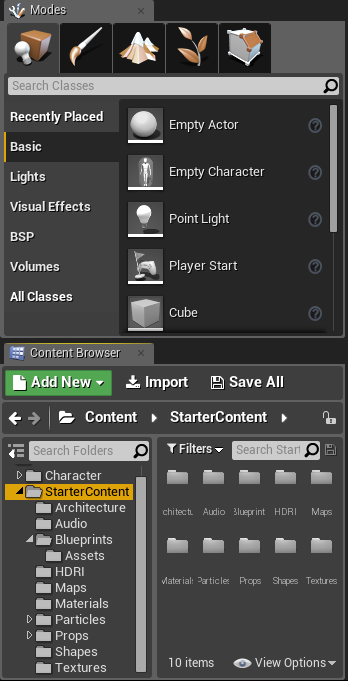
\includegraphics[scale=0.5]{Screeny/UeKrokPoKroku/UE-MyGame-Scene.png}
    \end{center}
    \caption{Krok po kroku - UE -  MyGame - Scena}
    \source{Zrzut ekranu z UnrealEngine}
\end{figure}

Kiedy już utworzymy swoją scenę i upewnimy się, że model postaci ma na czym stać, możemy kliknąć przycisk "play" (symbol trójkąta) z górnego panelu w celu sprawdzenia, czy wszystko działa poprawnie.

\newpage
\section{Krok 4 - Wspinaczka i kolizje}

Teraz kiedy mamu już gotową scenę, oraz postać, którą możemy poruszać możemy przejść do wspinaczki. Pierwsze co nam się w tym przypadku przyda to obszar kolizji, dzięki któremu postać będzie wiedziała kiedy zbliży się do powierzchni na którą może się wspiąć. Na początku powinniśmy w ustawieniach projektu zadeklarować „tracery" - funkcje, które będą śledzić czy i kiedy postać się do czegoś zbliża.

\begin{figure}[!htb]
    \begin{center}
    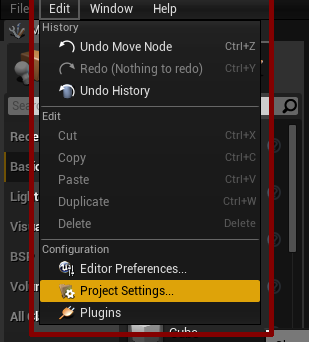
\includegraphics[scale=0.5]{Screeny/UeKrokPoKroku/UE-Climb-ProjectSettings.png}
    \end{center}
    \caption{Krok po kroku - UE - Ustawienia Projektu}
    Aby dostać się do ustawień projektu, należy kliknąć na zakładkę „Edit" w lewym górny rogu progamu, a następnie z listy wybrać opcję „Project settings".
    \source{Zrzut ekranu z UnrealEngine}
\end{figure}

Wyskoczy nam nowe okienko. Z panelu po lewej stronie wyszukujemy i wybieramy „Collision". W tym miejscu tworzymy dwa kanały. Jeden dla obiektu/postaci (SphereTracer), drugi dla znajdywania krawędzi (LedgeTracer). W obydwu przypadkach domyślną odpowiedź ustawiamy na „ignore".

\begin{figure}[!htb]
    \begin{center}
    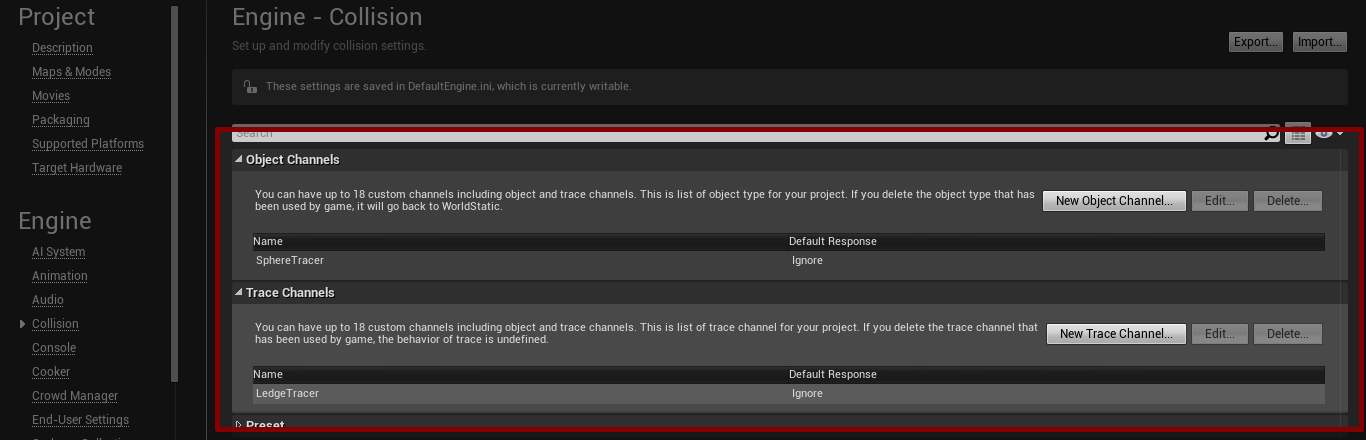
\includegraphics[scale=0.35]{Screeny/UeKrokPoKroku/UE-Climb-Collision.png}
    \end{center}
    \caption{Krok po kroku - UE -  Kolizje - Tworzenie tracerów}
    \source{Zrzut ekranu z UnrealEngine}
\end{figure}

\newpage
Następnie tworzymy obszar kolizyjny za pomocą sfery. W tym celu wyszukujemy i otwieramy plik CharacterBP. Ukaże nam się kolejne okno. W jego lewym górnym rogu powinna znajdować się lista komponentów. Tam dodajemy nowy komponent „Sphere Collision" i nazywamy go „SphereTracer". Klikamy na niego dwukrotnie - przeniesie nas to do kolejnego okna, gdzie będziemy mogli edytować obszar kolizji.

\begin{figure}[!htb]
    \begin{center}
    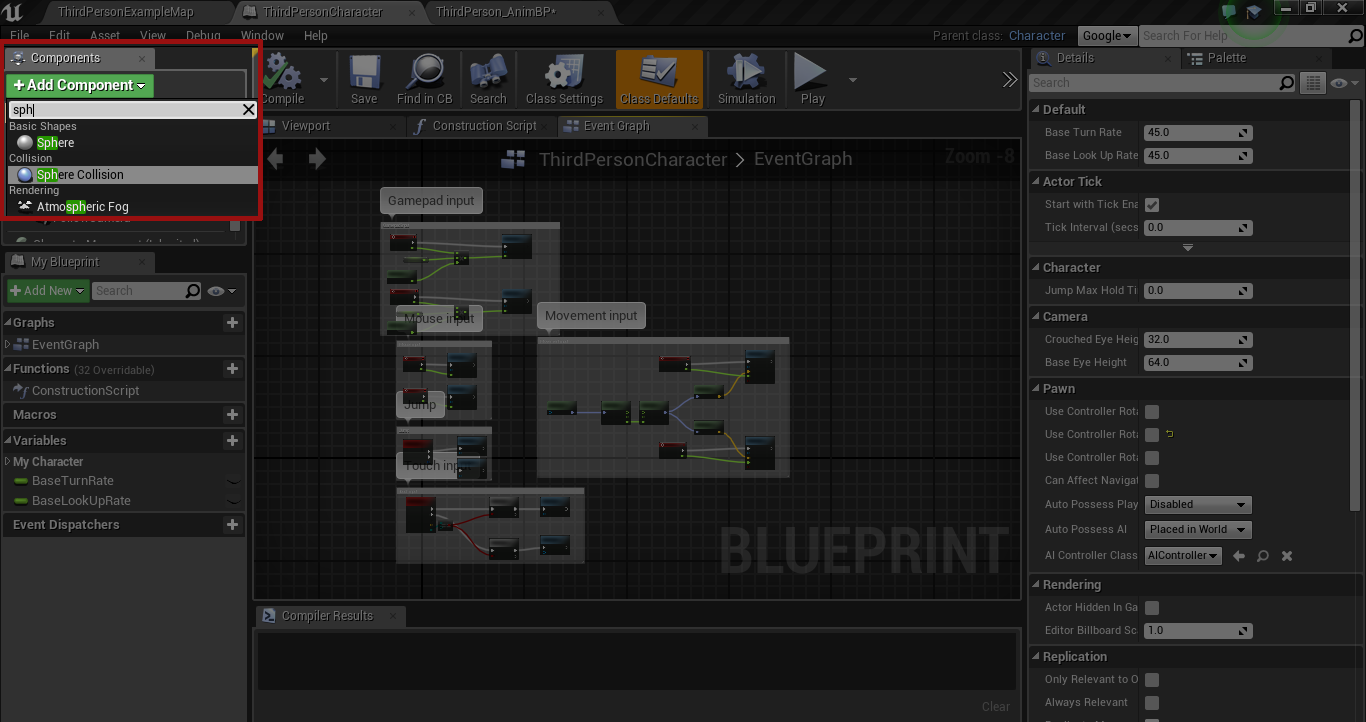
\includegraphics[scale=0.5]{Screeny/UeKrokPoKroku/UE-Climb-Sphere01.png}
    \end{center}
    \caption{Krok po kroku - UE - Kolizje - Tworzenie sfery}
    \source{Zrzut ekranu z UnrealEngine}
\end{figure}
\newpage

W menu po prawej stronie wyszukujemy zakładkę „Shape". Tam możemy zmienić promień naszej sfery powiększając lub pomniejszając obszar kolizji naszej postaci. Dla celów wspinaczkowych obszar ten został ustawiony na nieco większy niż postać.

\begin{figure}[!htb]
    \begin{center}
    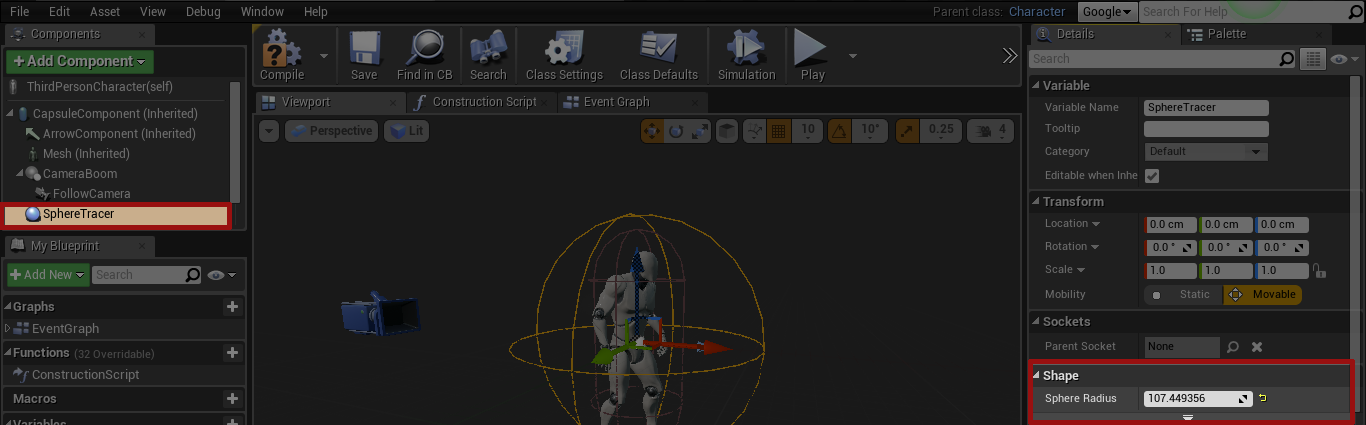
\includegraphics[scale=0.35]{Screeny/UeKrokPoKroku/UE-Climb-Sphere02.png}
    \end{center}
    \caption{Krok po kroku - UE - Kolizje - Edycja rozmiaru sfery}
    \source{Zrzut ekranu z UnrealEngine}
\end{figure}

Następnie również po prawej stronie wyszukujemy zakładkę „collision". Upewniamy się, że „Generate Overlap Events" zostało ustawione na „prawdę". Następnie „Collision Presets" zmieniamy na „Custom...". Upewniamy się, że „Object Type" został ustawiony na „SphereTracer". Następnie w „Collision Response" ustawiamy wszystko na „Ingore" - jedyne wyjątki stanową „LedgeTracer", który powinien być ustawiony na „Block", oraz „WorldStatic", który powinien być ustawiony na „Overlap".

\begin{figure}[!htb]
    \begin{center}
    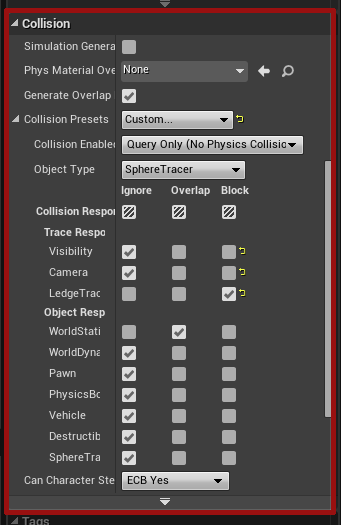
\includegraphics[scale=0.35]{Screeny/UeKrokPoKroku/UE-Climb-Sphere03.png}
    \end{center}
    \caption{Krok po kroku - UE - Kolizje - Edycja ustawień kolizji sfery}
    \source{Zrzut ekranu z UnrealEngine}
\end{figure}
\newpage

Teraz możemy powrócić do naszej sceny i wybrać obiekt na który gracz będzie mógł się wspinać. W tym celu klikamy na niego i w prawym menu szukamy zakładki „Collision". Upewniamy się, że „Generate Overlap Events" zostało ustawione na fałsz. Następnie „Collision Presets" zmieniamy na „Custom...". Upewniamy się, że „Object Type" został ustawiony na „WorldStatic". Następnie w „Collision Response" ustawiamy wszystko na „Block" - jedynie „SphereTracer" powinien być ustawiony na „Overlap".

\begin{figure}[!htb]
    \begin{center}
    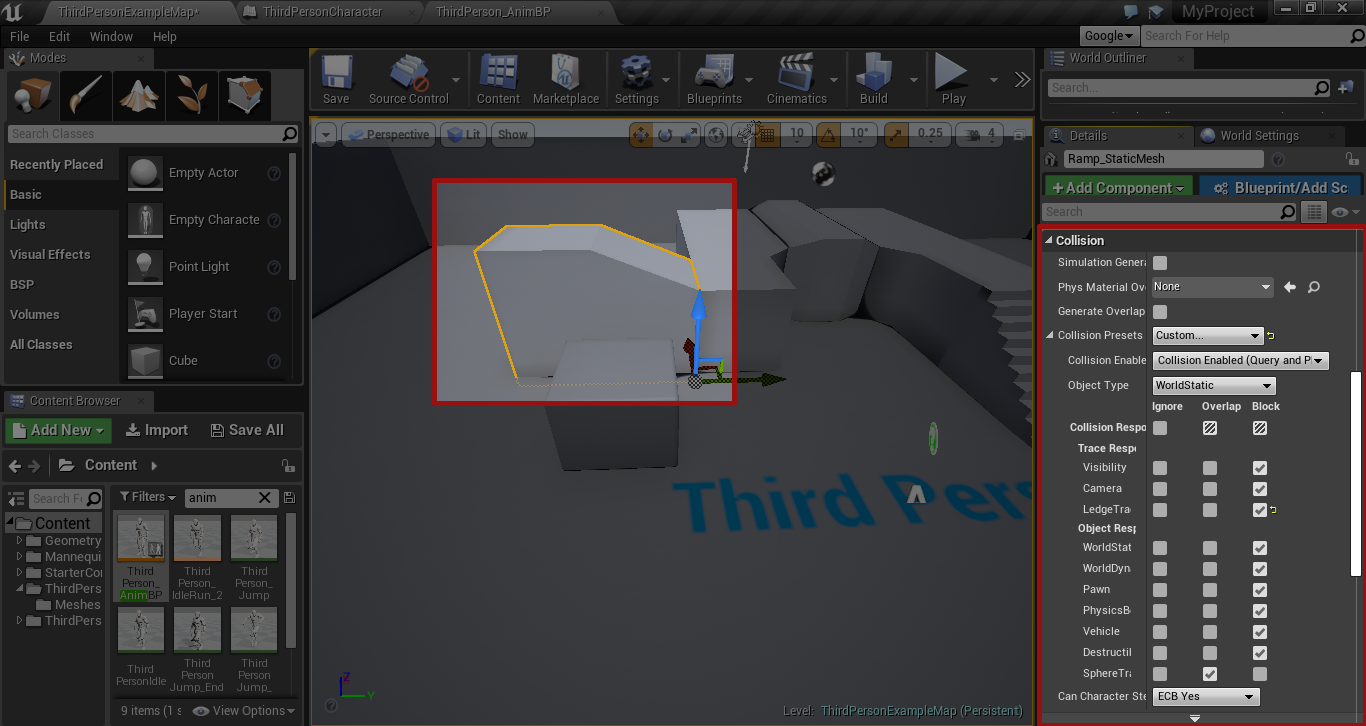
\includegraphics[scale=0.35]{Screeny/UeKrokPoKroku/UE-Climb-ObjectCollision}
    \end{center}
    \caption{Krok po kroku - UE - Kolizje - Ustawienia obiektu}
    \source{Zrzut ekranu z UnrealEngine}
\end{figure}

\newpage
\section{Krok 5 - Tracery}

Powracamy do pliku „CharacterBP". Tam w grafie zdarzeń tworzymy „Event Tick" - zdarzenie, które wykonuje się co klatkę w grze. Aby utworzyć jakąkolwiek akcję w grafach wystarczy kliknąć prawym przyciskiem myszy na wolnej przestrzeni. We wspomnianym zdarzeniu tworzymy linię od białego pięcioboku i tworzymy brancha. W nim z kolei od czerwonej kropki przy „condition" tworzymy kolejne połączenie. Z dostępnych opcji wybieramy „Promote to Variable" i powstałą wartość nazywamy „CanTrace".
W „Branchu" mamy dwie opcje. W przypadku, kiedy nie znaleźliśmy krawędzi na którą możemy się wspinać nic nie robi. Jeżeli jednak ją znaleźlimy wykonujemy dalsze instrukcje. Dlatego też tworzymy kolejną linię tylko od prawdy i tworzymy „sequence".

\begin{figure}[!htb]
    \begin{center}
    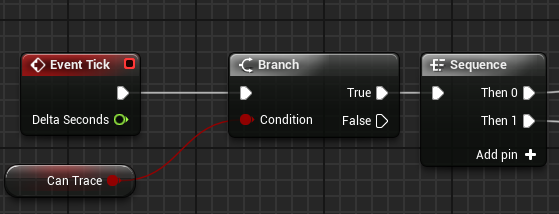
\includegraphics[scale=0.5]{Screeny/UeKrokPoKroku/UE-Tick}
    \end{center}
    \caption{Krok po kroku - UE - Tracery - Tick}
    \source{Zrzut ekranu z UnrealEngine}
\end{figure}

\newpage
Następnie musimy powiedzieć programowi kiedy możliwość śledzenia jest prawdziwa, a kiedy nie. W tym celu obok w grafie zdarzeń tworzymy kolejne dwa zdarzenia. W tym celu klikamy raz lewym klawiszem myszy na SphereTracer w menu komponentów, a następnie prawym klawiszem myszy w wolnej przestrzeni grafu zdarzeń. W ten sposób tworzymy „Add on component begin overlap" oraz „Add on component end overlap". Następnie od każdego z nich od białego pięcioboku wyprowadzamy „set CanTrace". W przypadku rozpoczęcia przenikania „CanTrace" ustawiamy na fałsz. W przypadku zakończenia przenikania „CanTrace" ustawiamy na prawdę.

\begin{figure}[!htb]
    \begin{center}
    \includegraphics[scale=0.5]{Screeny/UeKrokPoKroku/UE-canTrace}
    \end{center}
    \caption{Krok po kroku - UE - Tracery - Zdarzenia „Can Trace"}
    \source{Zrzut ekranu z UnrealEngine}
\end{figure}

Nie każdy na każdą ścianę się wespnie. Musimy też znać wysokość ściany aby wiedzieć jak wysoko unieść naszą postać. „Sequence" pozwoli nam wyegzekwować dwa tracery jednocześnie. Obie opcje mają taki sam trzon - został on przedstawiony na obrazku poniżej.

\begin{figure}[!htb]
    \begin{center}
    \includegraphics[scale=0.5]{Screeny/UeKrokPoKroku/UE-Tracer}
    \end{center}
    \caption{Krok po kroku - UE - Tracery - Trzon}
    \source{Zrzut ekranu z UnrealEngine}
\end{figure}

\subsection{Wysokość}

W obu przypadkach na początku musimy zmodyfikować wektor sfery. W tym celu od żółtej kropki koło „End" w „SphereTraceByChannel" prowadzimy linię i wybieramy „make vector". Dla czystości kodu możemy kliknąć na nowopowstały wektor prawym przyciskiem myszy i wybrać „Collapse to Macro". Nazywamy go „LedgeTracer". Następnie możemy w niego wejść i zacząć go modyfikować. W rezultacie powinien wyglądać tak jak na obrazku poniżej.

\begin{figure}[!htb]
    \begin{center}
    \includegraphics[scale=0.4]{Screeny/UeKrokPoKroku/UE-HeightMacro}
    \end{center}
    \caption{Krok po kroku - UE - Tracery - Wysokość - Macro}
    Liczba, którą dodajemy (200) jest liczbą określającą wysokość sfery, t.j. jest najwyższym punktem tracera. Liczba przy mnożeniu (70) określa jak daleko od postaci ma znajdować się tracer. Liczba zdefiniowana w "distance" jest długością tracera.
    \source{Zrzut ekranu z UnrealEngine}
\end{figure}
\newpage
„Start" i „End" z „LedgeTracer" powinniśmy odpowiednio połączyć ze „Startem" i „Endem" w „SphereTraceByChannel". Ostatnia rzecz jaką powinniśmy zrobić jest przeciągnięcie linii od żółtej kropki koło „Impact Point" w „Break Hit Result", wybranie opcji „promote to variable", nazwanie nowopowstałego okienka LedgeHeight i dołączenie do niego opcji "prawda" z brancha. Powinno to wyglądać tak jak na obrazku poniżej.

\begin{figure}[!htb]
    \begin{center}
    \includegraphics[scale=0.5]{Screeny/UeKrokPoKroku/UE-Height}
    \end{center}
    \caption{Krok po kroku - UE - Tracery - Wysokość}
    \source{Zrzut ekranu z UnrealEngine}
\end{figure}
\newpage

\subsection{Odległość od ściany}

Wygląda bardzo podobnie do wysokości. Również możemy utworzyć nowy wektor i również możemy go zwinąć do macro. Tym razem nazywamy go „WallTracer". Jego zawartość powinna wyglądać tak jak na obrazku poniżej

\begin{figure}[!htb]
    \begin{center}
    \includegraphics[scale=0.5]{Screeny/UeKrokPoKroku/WallMacro}
    \end{center}
    \caption{Krok po kroku - UE - Tracery - Odległość od ściany - Macro}
    \source{Zrzut ekranu z UnrealEngine}
\end{figure}

\newpage
Tak jak w poprzednim przypadku „Start" i „End" z „WallTracer" powinniśmy odpowiednio połączyć ze „Startem" i „Endem" w „SphereTraceByChannel". Następnie w „Break Hit Result" awansujemy na zmienne „Impact Point" nazywając ją „WallTraceImpact", oraz „Normal" nazywając „WallNormal". Następnie „prawdę" z brancha łączymy z „WallTraceImpact", a ten następnie z „WallNormal". Całość powinna wyglądać tak jak na rysunku poniżej.

\begin{figure}[!htb]
    \begin{center}
    \includegraphics[scale=0.35]{Screeny/UeKrokPoKroku/UE-WallTracer}
    \end{center}
    \caption{Krok po kroku - UE - Tracery - Odległość od ściany}
    \source{Zrzut ekranu z UnrealEngine}
\end{figure}
\newpage
Jeżeli wszystko wykonaliśmy poprawnie po kliknięciu „play" na ekranie powinny nam się pojawić czerwone sfery koło postaci. Zmienią one kolor na zielony kiedy zbliżymy się do ściany, która została ustawiona do wspinaczki.

\begin{figure}[!htb]
    \begin{center}
    \includegraphics[scale=0.35]{Screeny/UeKrokPoKroku/spherecollision}
    \end{center}
    \caption{Krok po kroku - UE - Tracery - Końcowy efekt}
    \source{Zrzut ekranu z UnrealEngine}
\end{figure}

\section{Krok 6 - Chwytanie}

Teraz kiedy już nasza postać wykrywa ściany do wspinaczki możemy zająć się chwytaniem krawędzi. Na początek stworzymy nowy interfejs. Aby to zrobić, w przeglądarce zawartości (w lewym dolnym rogu) klikamy przycisk „Add New", następnie rozwijamy „Bueprints" i wybieramy „Blueprint interface". Nazywamy go „CharMoveInterface" i od razu go otwieramy.

W prawym górym rogu nowo otwartego okienka mamy możliwość dodania nowych funkcji. Pierwszą jaką dodamy nazywamy CanGrabLedge$\_$BI. W nią w „Inputs" dodajmy wartość „Boolean" o nazwie "CanGrab$\_$BI.

Wracamy do „CharacterBP". Z górnego menu klikamy na „Class Settings". Powinno nam się pojawić menu po prawej. Tam w zakładce Interfaces klikamy „Add" i dodajemy nasz niedawno utworzony interfejs. Tę samą operację wykonujemy w pliku „CharacterAnimBP".

Ponownie wracamy do „CharacterBP" i do „Ledge Height Tracer". Od „Ledge Height" tworzymy linię i wybieramy opcję „DoOnce". Wracamy do „CharacterAnimBP". Tam tworzymy nowe zdarzenie „Event Can Grab Ledge BI". Następnie przeciągamy od czerwonej kropki linię i wybieramy opcję „Promote to variable". Naszą nową zmienną nazywamy „CanGrab".

\begin{figure}[!htb]
    \begin{center}
    \includegraphics[scale=0.5]{Screeny/UeKrokPoKroku/CanGrabInterface}
    \end{center}
    \caption{Krok po kroku - UE - Chwytanie - Interfejs}
    \source{Zrzut ekranu z UnrealEngine}
\end{figure}

\newpage
Wracamy do pliku „CharacterBP". Od zadeklarowanego niedawno „DoOnce" przeciągamy linie i tworzymy schemat zgodny z poniższymi rysunkami.

\begin{figure}[!htb]
    \begin{center}
    \includegraphics[scale=0.5]{Screeny/UeKrokPoKroku/GrabLedge}
    \end{center}
    \caption{Krok po kroku - UE - Chwytanie}
    \source{Zrzut ekranu z UnrealEngine}
\end{figure}

\begin{figure}[!htb]
    \begin{center}
    \includegraphics[scale=0.5]{Screeny/UeKrokPoKroku/WallGoToLocation}
    \end{center}
    \caption{Krok po kroku - UE - Chwytanie - Przysuwanie postaci do krawędzi}
    Widok rozwiniętego makro „WallGoToLocation"
    \source{Zrzut ekranu z UnrealEngine}
\end{figure}

\newpage
Po raz kolejny wracamy do „CharacterAnimBP", tym razem przechodzimy do Animacji Grafu. Tam klikamy prawym przyciskiem myszy na tło i wybieramy „Add state...". Nasz nowy stan możemy nazwać „LedgeGrab". Klikamy na niego dwukrotnie, aby dodać animacje. Aby to zrobić wystarczy przeciągnąć linię od kafelka „Final Animation Pose" i wybrać animację „LedgeGrabPlaceHolder".

Powracamy do głównego ekranu Animacji Grafu. Do nowego stanu musimy dodać połączenia, aby postać wiedziała kiedy ma się krawędzi chwytać.

\begin{figure}[!htb]
    \begin{center}
    \includegraphics[scale=0.5]{Screeny/UeKrokPoKroku/UE-AnimGraph}
    \end{center}
    \caption{Krok po kroku - UE - Chwytanie - Graf Animacji}
    Na obrazku przedstawiono połączenia do stanu chwytania oraz logikę, jaką należy do tych połączeń dodać.
    \source{Zrzut ekranu z UnrealEngine}
\end{figure}

\newpage

\section{Krok 7 - Puszczanie krawędzi}

Na początek przypiszmy klawisz dla puszczania krawędzi w ustawieniach projektu. Robimy to w sekcji „Input” w „Action Mappings”. Naszą nową akcję nazywamy „Crouch” i przypisujemy do niej klawisz „s”.

Następnie wracamy do „CharacterBP”. Tworzymy nowe zdarzenie, które nazywamy „LetGoOfLedge”. Następnie tworzymy połączenia tak jak na obrazku poniżej.

\begin{figure}[!htb]
    \begin{center}
    \includegraphics[scale=0.5]{Screeny/UeKrokPoKroku/LetGoOfLedge}
    \end{center}
    \caption{Krok po kroku - UE - Puszczanie krawędzi}
    \source{Zrzut ekranu z UnrealEngine}
\end{figure}

Teraz możemy przypisać zdarzenie do naszego przycisku „Crouch”. W tym celu tworzymy nową akcję i schemat do niej tak jak na obrazku poniżej.

\begin{figure}[!htb]
    \begin{center}
    \includegraphics[scale=0.5]{Screeny/UeKrokPoKroku/Crouch}
    \end{center}
    \caption{Krok po kroku - UE - Puszczanie krawędzi - Crouch}
    \source{Zrzut ekranu z UnrealEngine}
\end{figure}

W tym momencie postać po oderwaniu się od ściany nie będzie mogła wespnąć się ponownie. Dzieje się tak za sprawą „doOnce”, które łączyło nasze tracery z grafem chwytania krawędzi. W tym miejscu możemy ją zastąpić branchem, z którego linie prowadzimy od wartości „true” do brancha w „Grab Ledge”. Zanim jednak dodamy warunek, przechodzimy do szkieletu naszej postaci.

Upewniamy się, że w prawym górnym rogu został zaznaczony „skeleton”. Następnie po lewej stronie klikamy prawym przyciksiem myszy na „Pelvis” i wybieramy „Add socket”. Nazywamy go „HipSocket” i upewniamy się, że taka nazwa figuruje również w panelu po prawej stronie.

\begin{figure}[!htb]
    \begin{center}
    \includegraphics[scale=0.5]{Screeny/UeKrokPoKroku/HipSocket}
    \end{center}
    \caption{Krok po kroku - UE - Puszczanie krawędzi - HipSocket}
    \source{Zrzut ekranu z UnrealEngine}
\end{figure}

Wracamy do „CharacterBP” i do naszego brancha. Jako warunek tworzymy schemat widoczny poniżej (po prawej), które później zwijamy do macro i nazywamy „HipToLedgeDistance”. Całość powinna wyglądać tak jak po lewej stronie obrazka, przy czym podane liczby możemy modyfikować w celu uzyskania najlepszego efektu przybliżenia do krawędzi.

\begin{figure}[!htb]
    \begin{center}
    \includegraphics[scale=0.5]{Screeny/UeKrokPoKroku/HipToLedgeDistanceMacro}
    \end{center}
    \caption{Krok po kroku - UE - Puszczanie krawędzi - Dystans do krawędzi}
    \source{Zrzut ekranu z UnrealEngine}
\end{figure}

\newpage
\section{Krok 8 - Wspinanie}

Wracamy do ekranu głównego naszego projektu. Ponownie musimy przypisać klawisz dla akcji, tym razem dla wspinania. Robimy to w tym samym miejscu co „Crouch”. Tym razem akcje nazywamy „Climb” i przypisujemy jej klawisz spacji. Zamykamy okno.

W przeglądarce zawartości wyszukujemy plik „ClimbLedgePlaceHolder” i otwieramy go. Wewnątrz w dolnym lewym panelu w zakładce „Root Motion” wyszukujemy „Enable Root Motion”, a następnie upewniamy się, że jest zaznaczony. Zapisujemy plik i z niego wychodzimy. 

Następnie klikamy prawym przyciskiem myszy na plik, z którego wyszliśmy i w sekcji „create” wybieramy „create AnimMontage”. Nie zmieniając nazwy pliku zatwierdzamy go i otwieramy. W dolnym środkowym panelu wyszukujemy sekcję „Notifies”. Następnie klikamy prawym przyciskiem myszy na pasku, który znajduje się w tej sekcji, wybieramy „Add notify” i następnie „New notify”, który nazywamy „ClimbingEnd”. Upewniamy się, że znajduje się on na końcu paska – sygnalizować on nam będzie koniec animacji wspinaczki. Następnie w panelu po prawej stronie, w sekcji „Event” zmieniamy „Montage Tick Type” na „Branching Point”.

\begin{figure}[!htb]
    \begin{center}
    \includegraphics[scale=0.5]{Screeny/UeKrokPoKroku/MontageNotify}
    \end{center}
    \caption{Krok po kroku - UE - Wspinanie - Montaż wspinaczki}
    \source{Zrzut ekranu z UnrealEngine}
\end{figure}

\newpage
Wracamy do dolnego środkowego panelu, a następnie wyszukujemy i naciskamy przycisk lupy w sekcji „Montage” . Dodajemy nową grupę „TP\_Slot”, a w niej dodajemy nowy slot „TP”. Zamykamy okienko i w tej samej sekcji zmieniamy „DefaultGroup” na „TP\_Slot.TP". Zapisujemy i przechodzmy do „CharacterAnimBP”.

W dolnym panelu, w zakładce „My Blueprint” wyszukujemy i klikamy dwukrotnie „AnimGraph”. Przeciągamy linię od „Locomotion” aby dodać „DefaultSlot”, który następnie łączym z „Final Animation Pose”.  Upewniamy się, że slot jest zaznaczony, a następnie w prawym dolnym panelu w „Slot Name” zmieniamy nazwę na „DefaultGroup.TP”

\begin{figure}[!htb]
    \begin{center}
    \includegraphics[scale=0.5]{Screeny/UeKrokPoKroku/AnimGraphSlot}
    \end{center}
    \caption{Krok po kroku - UE - Wspinanie - Sloty Grafu Animacji}
    \source{Zrzut ekranu z UnrealEngine}
\end{figure}
\newpage
Zapisujemy i przechodzimy do „CharacterAnimBP” do grafu zdarzeń. W tym miejscu stworzymy gra dla naszej wspinaczki, zgodny z rysunkiem poniżej.

\begin{figure}[!htb]
    \begin{center}
    \includegraphics[scale=0.5]{Screeny/UeKrokPoKroku/LedgeClimbingGraph}
    \end{center}
    \caption{Krok po kroku - UE - Wspinanie - Graf zdarzeń}
    \source{Zrzut ekranu z UnrealEngine}
\end{figure}

Ostatnią rzeczą, jaką musimy zrobić, to zmodyfikować graf skoku. W tym celu powracamy do „CharacterBP” i w grafie zdarzeń wyszukujemy „jump”. Graf modyfikujemy tak, by wyglądał jak na obrazku poniżej.

\begin{figure}[!htb]
    \begin{center}
    \includegraphics[scale=0.5]{Screeny/UeKrokPoKroku/JumpClimb}
    \end{center}
    \caption{Krok po kroku - UE - Wspinanie - Modyfikacja skoku}
    \source{Zrzut ekranu z UnrealEngine}
\end{figure}

\section{Krok 9 - Wykończenie}

Nasza postać potrafi się już poruszać, skakać, a nawet wspinać. Mamy też utworzoną scenę, którą w każdym momencie możemy wyedytować. Pozostało jeszcze kilka rzeczy, które możemy dodać do naszego projektu. Jedną z nich jest usunięcie widoku tracerów. Aby to zrobić wystarczy wejść w „CharacterBP”, i w obu tracerach, w „SphereTraceByChannel” zmienić wartość „Draw Debug Type” na „None”.

\subsection{Menu główne}

Aby utworzyć menu główne musimy stworzyć nowy poziom.W tym celu w wyszukiwarce zawartości klikamy „Add New” i wybieramy „Level”. Nazywamy go „MainMenu”, zatwierdzamy i klikamy na niego dwukrotnie. 

W nowym poziomie tworzymy widget dla naszego menu. W tym celu klikamy „Add New” $\rightarrow$ „User Interface” $\rightarrow$ „Widget Blueprint”. Nowy plik nazywamy „MenuBP” i klikamy na niego dwukrotnie.

\begin{figure}[!htb]
    \begin{center}
    \includegraphics[scale=0.35]{Screeny/UeKrokPoKroku/MainMenu}
    \end{center}
    \caption{Krok po kroku - UE - Wykończenie - Menu główne}
    \source{Zrzut ekranu z UnrealEngine}
\end{figure}

Po lewej stronie mamy listę rzeczy, które możemy uszyć w naszym widoku. Przy prostym menu będziemy używać tylko „Button” i „Text”. Wystarczy przeciągnąć odpowiedni komponent na środek ekranu. W naszym przypadku stworzymy przycisk dla poziomu i przycisk wyłączenia gry.

Gdy zaznaczymy przycisk, po prawej stronie wyświetli się nam kilka opcji. Pierwsze, na co powinniśmy zwrócić uwagę, to „Anchors” w zakładce „Slot”. Aby menu poprawnie się wyświetlało warto po każdej zmianie pozycji przycisku kliknąć na „Anchors” i wybrać wycentrowaną opcję. Kolejną ważną sekcją jest „Events”. Aby dodać akcję wystarczy kliknąć znak plusa przy „OnClicked”.

Zostaniemy automatycznie przeniesieni do grafu zdarzeń naszego menu. Widzimy, że utworzył się kafelek dla naszego przycisku. Wystarczy, że przeciągniemy teraz od niego linię i dodamy którąś z wbudowanych funkcji - „Quit game” lub „Open Level” odpowiednio dla zakończenia gry lub otwarcia konkretnego poziomu. Przy tym drugim warto wcześniej spojrzeć jak nazywa się poziom, na którym stworzyliśmy swoją scenę.

\begin{figure}[!htb]
    \begin{center}
    \includegraphics[scale=0.5]{Screeny/UeKrokPoKroku/MainMenuEvent}
    \end{center}
    \caption{Krok po kroku - UE - Wykończenie - Menu główne - graf zdarzeń}
    \source{Zrzut ekranu z UnrealEngine}
\end{figure}

Warto ustawić jeszcze daną scenę jako domyślną podczas ładowania gry. W tym celu udajemy się do ustawień projektu i „Maps \& Modes”. W sekcji „Default Maps” możemy ustawić odpowiedni poziom dla „Game Default Map” (domyślny poziom po załadowaniu gry) oraz „Editor Startup Map” (domyślny poziom po załadowaniu projektu).

\newpage
\subsection{Pauza}

Początkowo menu z pauzą tworzymy analogicznie do menu głównego. Rozpoczynamy go od tworzenia widgetu, a następnie edytujemy go w sposób jaki tylko chcemy. Możemy dodać takie przyciski jak powrót, wyjście do menu (otwarcie poziomu „MainMenu") czy wyjście z gry. Następnie dodajemy zdarzenia do przycisków. Dla powrotu do gry stosujemy poniższy graf.

\begin{figure}[!htb]
    \begin{center}
    \includegraphics[scale=0.5]{Screeny/UeKrokPoKroku/PauseButton}
    \end{center}
    \caption{Krok po kroku - UE - Wykończenie - Pauza - Graf zdarzeń przycisku}
    \source{Zrzut ekranu z UnrealEngine}
\end{figure}

Pauzę trzeba w jakiś sposób aktywować. Aby to zrobić na początku dodajemy klawisz wejściowy „p” w „Inputs” w ustawieniach projektu. W naszym projekcie nazywamy go „Menu”. Następnie przechodzimy do pliku „CharacterBP” i dodajemy do niego poniższy graf.

\subsection{Obszar śmierci}

Gdy tworzymy gry platformowe istnieje prawdopodobieństwo, że postać spadnie w przepaść. W takich przypadkach przydaje się tzw. obszar śmierci. Aby go stworzyć w przeglądarce zawartości dodajemy nowy „Blueprint Class” z klasą rodzicielską „Actor”. Po odpowiednim nazwaniu go, klikamy na niego dwukrotnie. 

Wewnątrz, po lewej stronie mamy menu komponentów. Dodajemy do niego „Box collision”, a następnie już w przeglądarce przeciągamy go na „DefaultSceneRoot”, dzięki czemu obszar ten będzie całkowicie niewidzialny dla gracza. 

Następnie przechodzimy do grafu zdarzeń. Zaczynamy od utworzenia zdarzenia „ActorBeginOverlap”. Tutaj należy zdecydować co właściwie strefa śmierci ma robić. Na poniższym obrazku znajduje się przeniesienie postaci do z góry ustalonej lokacji początkowej poziomu.

\begin{figure}[!htb]
    \begin{center}
    \includegraphics[scale=0.5]{Screeny/UeKrokPoKroku/LevelGraph}
    \end{center}
    \caption{Krok po kroku - UE - Wykończenie - Obszar śmierci }
    \source{Zrzut ekranu z UnrealEngine}
\end{figure}

Następnie wystarczy umieścić nasz obszar śmierci w naszym poziomie tam, gdzie gracz nie powinien się znaleźć. Należy pamiętać, że postać zostanie przeniesiona automatycznie po zetknięciu się z obszarem śmierci.

\subsection{Drzwi do menu}

Warto byłoby zakończyć poziom przejściem do kolejnego poziomu lub do menu, z którego można by przechodzić do innych poziomów. Obszar ten wykonuje się analogicznie do obszaru śmierci – różnica tkwi w grafie zdarzeń – zamiast „Teleport” ustawiamy „Open Level”, a wartość w nim ustawiamy na poziom naszego menu głównego.

\begin{figure}[!htb]
    \begin{center}
    \includegraphics[scale=0.5]{Screeny/UeKrokPoKroku/Door}
    \end{center}
    \caption{Krok po kroku - UE - Wykończenie - Przejście}
    \source{Zrzut ekranu z UnrealEngine}
\end{figure}

\subsection{Pakowanie gry}

W momencie, w którym zdecydujemy, że nasza gra jest gotowa, można ją spakować i udostępnić innym. W tym celu przechodzimy do ekranu głównego projektu. Następnie wybieramy zakładkę „File” i „Package Project”. W tym miejscu mamy wybór na jaką platformę chcemy naszą grę wyeksportować. Kiedy już zdecydujemy wystarczy kliknąć na daną opcję. Po wybraniu miejsca, w którym ma powstać spakowana gra, reszta procesu wykona się automatycznie.

\chapter{Podsumowanie tworzenia gier dla obu silników}

W tym rozdziale porównamy  oba silniki, ich mocne i słabe strony. Określimy również w jakich okolicznościach dany silnik jest preferowanym narzędziem.

\section{Multiplatformowość}

Twórcy Unity chwalą się, że gry w Unity mogą zostać wydane na ponad 21 platform. Wystarczy jedno kliknięcie, aby stworzyć build gry na komputery osobiste, wszelkiego rodzaju konsole, smartfony, a nawet przeglądarki internetowe. Ostatnimi czasy nawet wydanie gry na urządzenia VR (Virtual Reality) zostało dodane jako opcja.

Unreal Engine prezentuje się pod tym względem dużo gorzej. Ma jedynie opcje wydania gier na komputery osobiste, urządzenia mobilne, przeglądarki internetowe i urządzenia VR. Taka multiplatformowość wymaga jednak dużo więcej wysiłku ze strony użytkownika.

Jeśli chcemy wydać grę na wiele platform Unity jest preferowanym wyborem.

\section{Przystępność}

Jeśli chodzi o interfejs użytkownika, Unity ma bardzo przejrzysty i wygodny interfejs. Zdecydowaną większość działań wykonuje się na ekranie głównym. Nawet pierwszy raz używając silnika można intuicyjnie nawigować po wszystkich opcjach.
W przypadku, w którym nie odpowiada nam obecny layout interfejsu możemy bez trudu zmienić konfigurację wszystkich menu.
Dodać należy fakt, że wszystkie elementy silnika są bardzo dobrze udokumentowane, a w przypadku wątpliwości można odwołać się do ogromnej ilości wszelkiej maści tutoriali i forów tworzonych przez społeczność Unity.

Unreal Engine mimo wielu podobieństw do Unity posiada dużo bardziej rozbudowany, skomplikowany interfejs. Każdy system wewnątrz silnika otwierany jest w osobnym okienku, lub karcie. W przypadku wyboru opcji programowania w C++ trzeba używać programów z zewnątrz UE, co jeszcze bardziej komplikuje sprawę. Taki interface może bardzo łatwo przytłoczyć początkującego użytkownika. Istnieje co prawda wbudowany w silnik samouczek, objaśniający wszystkie części interface’u, jednak nie wyjaśnia on wszystkiego.
Z drugiej strony dzięki systemowi Blueprint’ów, przeciętny użytkownik silnika nie musi być zaznajomiony z żadnym językiem programowania.
Problem może pojawić się, gdy twórca gry nie do końca zrozumie sposobu działania funkcji. Niestety UE jest znany z niepełnej i niedokładnej dokumentacji, która nie pokrywa wszystkich funkcji dostępnych w silniku.

\section{Grafika}

Unity od wersji 5.0 posiada wiele zaawansowanych opcji graficznych, takich jak wysokiej jakości shadery, lightmapy, filtry anizotropowe. Obsługuje również efekty takie jak głębia terenu, czy motion blur, zoptymalizowane pod DirectX 11. Umożliwia to stworzenie gier wyglądem konkurującymi z produkcjami światowej klasy.
Mimo to Unreal Engine nadal ma pod tym względem znaczącą przewagę. Polega ona na uproszczonym procesie tworzenia grafiki. Tworzenie wysokiej jakości grafiki w Unity, wymaga wiele pracy w zewnętrznym programie graficznym. W Unreal Engine, dzięki systemowi Blueprint’ów i idei skryptowania wizualnego, wystarczy kilka kliknięć myszką, aby osiągnąć znacznie lepsze efekty, przy mniejszym wysiłku. Tekstury w UE posiadają własny, rozbudowany edytor. Pozwala on nie tylko dowolnie modyfikować materiał, kolor i inne właściwości  tekstury, ale również kontrolować jej mapę UV. Dzięki temu, tekstura nie „rozjeżdża się” na trójwymiarowym obiekcie. Generowany teren, efekty cząsteczkowe (takie jak płomienie, czy pył unoszący się w powietrzu) oraz światło również przekraczają możliwości Unity. Dodatkowo Unreal Engine 4 posiada już wsparcie DirectX 12, co znacznie poprawia wydajność i zmniejsza czas renderowania grafiki.

\begin{figure}[!htb]
    \begin{center}
    \includegraphics[scale=0.5]{Screeny/UE_vs_Unity}
    \end{center}
    \caption{UnrealEngine a Unity - porównanie grafiki}
    \source{forum.unity3d.com}
\end{figure}

\section{Programowanie i zasoby}

Unity umożliwia programowanie w językach C\# i Unity Script. Pozwala to nie tylko elastyczność w wyborze. Same języki ułatwiają optymalizację gry, pozwalając na znaczące zmniejszenie wymagań systemowych.

Unreal Engine korzysta wyłącznie z języka C++. Mimo, że sam język jest łatwy do optymalizacji, by go używać potrzebny jest zewnętrzny edytor. Wyjściowym sposobem tworzenia kodu jest Blueprint, który nie zapewnia bezpośredniego dostępu do kodu. Mimo, że upraszcza proces tworzenia gry dla bardziej doświadczonych developerów, to znacznie utrudnia optymalizację gry.

\chapter{ Testowanie gier}

Wśród programistów gier panuje przekonanie, że tworzenie zautomatyzowanych testów do gier jest pozbawione sensu. Większość firm zatrudnia sztab testerów, którzy manualnie sprawdzają najdrobniejsze elementy danej gry. Wynika to z kilku wyjątkowych cech tworzenia gier.

Po pierwsze, zdecydowana większość logiki używanej w grach zależy od czynników, które nie są do końca deterministyczne. Oznacza to, że warunki w jakich użytkowana będzie gra często mogą być przypadkowe i niemożliwe do przewidzenia. Na przykład, gra może być uruchamiana na setkach różnych konfiguracji sprzętu. Przetestowanie każdej z nich jest niemożliwe. Dodajmy do tego fakt, że sprzęt może znajdować się w gorącym pomieszczeniu, co pogorszy jego osiągi. W tle mogą również być uruchomione inne programy, które zajmują zasoby danego sprzętu. To tylko kilka przykładów czynników nad którymi twórcy gier nie mają żadnej kontroli. Ustalenie standardu według którego możnaby napisac test, w takich warunkach jest niemal niewykonalne.

Innym problemem jest, że większość wyników produkowanych przez grę jest niemożliwa do zmierzenia.
W grach generowane są takie elementy jak grafika i dźwięk.  Skuteczność efektów wizualnych, jak i dźwiękowych jest rzeczą załkowicie subiektywną. Nie da się określić automatycznym testem czy muzyka jest dostatecznie głośna, lub czy dana tekstura wygląda dobrze w danym miejscu. Wszystko zależy od wizji twórców gry. W takim wypadku jedyny możliwy test, to test manualny.

Kolejną przeszkodą jest fakt, że w większości gier wszystkie mechaniki i podsystemy składają się na jedną spójną całość. W jednej z gier stworzonych na potrzeby tego projektu zaimplementowaliśmy mechanikę wspinaczki. Aby działała, zarówno fizyka gry, jak i animacje oraz kod wykrywający kolizję muszą działać poprawnie. W przypadku porażki nie sposób na pierwszy rzut oka określić, który z tych systemów zawiódł. Możemy napisać testy, które sprawdzą wszystkie po kolei, jednak wszelkie wyniki jakie dostaniemy będą wyrwane z kontekstu i nie powiedzą co się stało, gdy wszystkie czynniki złączyły się w jedną całość. W związku z tym tu również musimy zdać się na testowanie ręczne.

Mimo powyższych problemów, pisanie unit testów do gier nie jest całkowicie niemożliwe. Wymaga to jednak bardzo specyficznych warunków. Głównym warunkiem jest określenie testów jeszcze przed rozpoczeciem programowania samej gry. Jest to jednak niepraktyczne podejście, które wiąże ręce twórcom gry.

Gry stworzone na potrzeby projektu zostały przetestowane wyłącznie manualnie. Testowaliśmy głównie mechanikę skoku, wspinaczki i biegu, ponieważ są to główne elementy naszych gier.


% zakończenie
\summary
Oba silniki mają swoje zalety, jednak należy używać ich w odpowiednich sytuacjach.

Jeśli planujemy stworzyć mniejszy tytuł na jedną platformę, cechujący się wysokiej jakości grafiką, Unreal Engine jest bardzo dobrym wyborem.

W przypadku w którym chcemy stworzyć grę na wiele platform, albo dopiero zaczynamy przygodę z tworzeniem gier, przystępnośc interfejsu Unity, oraz elastyczność w wyborze języka programowania znacząco ułatwią nam stworzenie naszej pierwszej gry.

% załączniki (opcjonalnie):
%\appendix
%\chapter{Tytuł załącznika jeden}

%Treść załącznika jeden.

%\chapter{Tytuł załącznika dwa}

%Treść załącznika dwa.


% literatura (obowiązkowo):
\nocite{*}
\bibliographystyle{unsrt}
\bibliography{xml}

% spis tabel (jeżeli jest potrzebny):
\listoftables

% spis rysunków (jeżeli jest potrzebny):
\listoffigures

\oswiadczenie

\end{document}
